\documentclass[12pt,a4paper]{report}
\usepackage[T1]{fontenc}
\usepackage[utf8]{inputenc}
\usepackage[english]{babel}
\usepackage{lmodern}
\usepackage{amsmath,amssymb,mathtools}
\usepackage{booktabs}
\usepackage{tabularx}
\usepackage{longtable}
\usepackage{array}
\usepackage{multirow}
\usepackage{enumitem}
\usepackage{float}
\usepackage{siunitx}
\usepackage{microtype}
\usepackage[margin=2.5cm]{geometry}
\usepackage{graphicx}
\usepackage{caption}
\usepackage{placeins}
\usepackage{tikz}
\usetikzlibrary{arrows.meta}
\graphicspath{{figures/}{figures/rysunki/}}
\usepackage{setspace}
\usepackage{hyperref}
\hypersetup{colorlinks=true,linkcolor=black,urlcolor=blue,citecolor=black}
\usepackage[nameinlink,noabbrev]{cleveref}

\newcolumntype{L}[1]{>{\raggedright\arraybackslash}p{#1}}
\newcolumntype{C}[1]{>{\centering\arraybackslash}p{#1}}

\begin{document}
% EiTI-style title page (graphics from thesis/szablon, origin/task-b).
% Album numbers and supervisor left as placeholders until filled in.
\thispagestyle{empty}
\begin{center}

\includegraphics[width=\textwidth]{szablon/eiti/header-eng.png}\\[1.2em]
Institute of Radioelectronics and Multimedia Technology\\[2.2em]

\includegraphics[width=0.4\textwidth]{szablon/eiti/title-final-project.png}\\[1.0em]
Postgraduate diploma thesis\\
Deep Learning -- Applications in Digital Media\\[2.2em]
{\large
Combining Structured Knowledge Graphs with Patient-Level Statistical Evidence\\
for Link Prediction and Clinical Prediction}\\[2.0em]
{\LARGE
Marta Jasiewicz Badowska\\[0.35em]
Monika Oskard}\\[0.6em]
{\normalsize student record book number ---}\\[1.8em]
thesis supervisor\\[0.4em]
mgr inż. Grzegorz Gwardys\\
\vfill
WARSAW \the\year
\end{center}
\clearpage

\begin{abstract}
\noindent
Thesis title: Integrating Graph Neural Networks and Statistical Dependence for Pharmacotherapy Knowledge Graphs

\medskip


This thesis investigates how structured knowledge represented by a pharmacotherapy knowledge graph can
 be combined with explicit statistical evidence derived from patient-level data.
The problem is studied through two complementary tasks operating on a shared synthetic pharmacotherapy 
benchmark.
Task~A addresses directed link prediction, using patient-level observations to evaluate candidate 
relations in the graph.
Task~B addresses patient-level clinical endpoint prediction as node classification task, 
using the graph as a shared structural scaffold while individual 
patient observations instantiate the node-level input.

Both tasks combine graph neural representations with explicit statistical dependence information.
In Task~A, a heterogeneous graph encoder is fused with candidate-specific statistical context derived 
from patient observations.
In Task~B, heterogeneous message passing is augmented with endpoint-oriented statistical evidence, 
while different graph architectures, propagation depths, and residual connections are evaluated.
HCR-derived coefficients are used as representations of empirical dependence.

On the synthetic benchmark, the final Task~A model is consistently strong under 
the official five-scenario validation protocol, and ablations show that explicit 
statistical context substantially improves link prediction over the graph representation alone.
In Task~B, the statistical branch is most beneficial when deeper message passing loses predictive 
information, whereas residual connections preserve the same information within the graph pathway. 
%consequently, the two mechanisms are not always additive on the synthetic graph.

The generality of these observations is further examined through cross-domain experiments 
on real-world datasets.
On leakage-corrected Last-FM*, progressive addition of explicit candidate-specific context 
systematically improves ranking quality over a heterogeneous graph encoder alone.
On a Hetionet-derived endpoint-prediction proxy, the statistical branch is again 
particularly valuable for deeper models.
On the H2GB IEEE-CIS-G card-fraud graph, residual connections stabilise learning and the 
statistical branch further improves fraud detection relative to residual message passing 
alone on a graph structure different from the synthetic pharmacotherapy graph.

The results support a common methodological conclusion: structured graph representations and explicit empirical dependence provide complementary sources of information for both graph reconstruction and patient-level prediction.
Their relative contribution depends on the task and on how effectively the graph neural network preserves relevant information through message passing.
The proxy experiments provide methodological stress tests, but their 
findings should be interpreted cautiously before any application to clinical settings.

\medskip
\noindent\textbf{Keywords:}
knowledge graphs,
graph neural networks,
heterogeneous graphs,
link prediction,
clinical endpoint prediction,
Hierarchical Correlation Reconstruction,
pharmacotherapy.
\end{abstract}

\chapter*{Streszczenie}
\addcontentsline{toc}{chapter}{Streszczenie}

Tytuł pracy dyplomowej: Łączenie grafowych sieci neuronowych z empirycznymi 
zależnościami statystycznymi na farmakoterapeutycznym grafie wiedzy

\noindent
Przedmiotem pracy dyplomowej jest przetestowanie możliwości łączenia farmakoterapeutycznej 
wiedzy zakodowanej w formie grafu wiedzy (ang.\ knowledge graph) 
z danymi empirycznymi pacjentów. 
Zagadnienie to jest rozpatrywane na dwóch uzupełniających się zadaniach
w docelowym środowisku klinicznym.
Zadanie~A koncentruje się na predykcji krawędzi (ang.\ link prediction) w grafie mechanistycznym, 
z wykorzystaniem topologii grafu wiedzy oraz statystycznej wiedzy na temat zjawiska uzyskanej z 
danych pacjenckich.
Natomiast Zadanie~B ma wykorzystywać graf wiedzy do predykcji wystąpienia zdarzeń klinicznych, 
rozumianych jako zdarzenia wymagające interwencji klinicznej, wykorzystując graf jako 
wspólny szkielet strukturalny, podczas gdy obserwacje dotyczące poszczególnych pacjentów stanowią 
dane wejściowe na poziomie węzłów.

Oba zadania wykorzystują grafowe sieci neuronowe (ang.\ Graph Neural Networks) oraz dane empiryczne 
przekazane do modelu w formie statystyk, ze szczególnym uwzględnieniem oceny siły zależności między zmiennymi.
Implementacje w obu zadaniach różnią się docelowymi architekturami, głębokością message passingu, 
połączeniami rezydualnymi, a także sposobem wykorzystania gałęzi statystycznej w architekturze sieci.
W części statystycznej wspólnym mianownikiem jest jednak wykorzystanie metody inspirowanej Hierarchical Correlation 
Reconstruction (HCR), która umożliwia opis zależności pomiędzy zmiennymi różnych typów za pomocą 
ortonormalnych funkcji bazowych i odpowiadających im współczynników.
%, pozwalając uwzględniać zarówno proste, 
%jak i bardziej złożone struktury zależności.

Na syntetycznym grafie farmakoterapeutycznym finalny model Zadania~A wykazuje bardzo dobre wyniki 
w oficjalnym protokole pięciu scenariuszy, a ablacja pokazuje, że jawny kontekst statystyczny 
istotnie poprawia predykcję krawędzi względem samej reprezentacji grafu.
W Zadaniu~B moduł statystyczny przynosi największe korzyści w sytuacjach, gdy głębsze 
warstwy message passingu prowadzą do utraty informacji predykcyjnych, 
podczas gdy połączenia rezydualne pozwalają zachować te informacje w obrębie ścieżki grafowej.
%W rezultacie na grafie syntetycznym działanie obu mechanizmów nie zawsze się sumuje.

Ogólny charakter tych obserwacji zweryfikowano dodatkowo na rzeczywistych zbiorach międzydomenowych.
W przypadku Last-FM* (z korektą wycieku danych) stopniowe dodawanie kontekstu 
specyficznego dla kandydata systematycznie poprawia jakość rankingu względem samego enkodera grafu 
heterogenicznego.
W eksperymencie predykcji punktów końcowych na Hetionet, gałąź statystyczna 
ponownie okazuje się szczególnie przydatna przy głębszych warsztwach modeli grafowych.
Na heterogenicznym grafie transkacji kartowych z znacznikiem fraud
 H2GB IEEE-CIS-G, połączenia rezydualne stabilizują uczenie, a gałąź statystyczna dodatkowo 
 poprawia detekcję oszustw względem samego message passingu z połączeniami rezydualnymi, 
 przy strukturze grafu odmiennej od syntetycznego szkieletu.

Wyniki potwierdzają wspólny wniosek metodologiczny: 
ustrukturyzowane reprezentacje grafów i jawna informacja o zależnościach 
empirycznych stanowią uzupełniający się zestaw źródeł informacji zarówno do rekonstrukcji grafów, 
jak i predykcji na poziomie pacjenta.
Ich względny wkład zależy od zadania oraz od tego, jak skutecznie grafowa sieć neuronowa zachowuje 
istotne informacje podczas kolejnych etapów propagacji i agregacji informacji w grafie.
Eksperymenty na zbiroach rzeczywistych i międzydomenowych są metodologicznymi testami obciążeniowymi, 
jednak ich wyniki należy interpretować ostrożnie przed jakimkolwiek zastosowaniem w realnych 
warunkach klinicznych.

\medskip
\noindent\textbf{Słowa kluczowe:}
grafy wiedzy,
grafowe sieci neuronowe,
grafy heterogeniczne,
predykcja linków,
predykcja klinicznych punktów końcowych,
Hierarchical Correlation Reconstruction,
farmakoterapia.

\tableofcontents

\chapter*{List of Symbols and Abbreviations}
\addcontentsline{toc}{chapter}{List of Symbols and Abbreviations}
\label{ch:symbols}

\noindent
Abbreviations used in the thesis are collected in Table~\ref{tab:symbols-abbrev}.
Mathematical symbols are defined at first use in the text.

\begin{longtable}{@{}L{3.35cm}lL{7.6cm}@{}}
\caption{Symbols and abbreviations by category.}
\label{tab:symbols-abbrev}\\
\toprule
Category & Abbreviation & Meaning \\
\midrule
\endfirsthead
\toprule
Category & Abbreviation & Meaning \\
\midrule
\endhead
\midrule
\multicolumn{3}{r}{\emph{Continued on next page}} \\
\endfoot
\bottomrule
\endlastfoot
% --- Clinical ---
\multirow{15}{=}{\raggedright Clinical and pharmacological}
  & ADR & Adverse Drug Reaction \\
  & AKI & Acute Kidney Injury \\
  & DILI & Drug-Induced Liver Injury \\
  & CKD & Chronic Kidney Disease \\
  & CNS & Central Nervous System \\
  & GI & Gastrointestinal \\
  & DDI & Drug--Drug Interaction \\
  & ALT & Alanine Aminotransferase \\
  & AST & Aspartate Aminotransferase \\
  & NSAID & Non-Steroidal Anti-Inflammatory Drug \\
  & ACEi & Angiotensin-Converting Enzyme Inhibitor \\
  & ARB & Angiotensin Receptor Blocker \\
  & SSRI & Selective Serotonin Reuptake Inhibitor \\
  & SNRI & Serotonin--Norepinephrine Reuptake Inhibitor \\
  & EHR & Electronic Health Record \\
\midrule
% --- Graph / ML ---
\multirow{16}{=}{\raggedright Graph, machine learning and computation}
  & KG & Knowledge Graph \\
  & CKG & Collaborative Knowledge Graph \\
  & DAG & Directed Acyclic Graph \\
  & GNN & Graph Neural Network \\
  & GCN & Graph Convolutional Network \\
  & R-GCN & Relational Graph Convolutional Network \\
  & GAT & Graph Attention Network \\
  & HGT & Heterogeneous Graph Transformer \\
  & GraphSAGE & Graph Sample-and-Aggregate architecture \\
  & HCR & Hierarchical Correlation Reconstruction \\
  & MLP & Multilayer Perceptron \\
  & PyG & PyTorch Geometric \\
  & KGAT & Knowledge Graph Attention Network \\
  & LightGCN & Light Graph Convolutional Network \\
  & 1-WL & One-Dimensional Weisfeiler--Lehman Test \\
  & LP & Link Prediction \\
\midrule
% --- Stats / eval ---
\multirow{17}{=}{\raggedright Statistics and evaluation}
  & AP & Average Precision \\
  & AUROC & Area Under the Receiver Operating Characteristic Curve \\
  & ROC & Receiver Operating Characteristic \\
  & PR & Precision--Recall \\
  & TPR & True Positive Rate \\
  & FPR & False Positive Rate \\
  & BCE & Binary Cross-Entropy \\
  & MI & Mutual Information \\
  & NMI & Normalized Mutual Information \\
  & PMI & Pointwise Mutual Information \\
  & NPMI & Normalized Pointwise Mutual Information \\
  & CDF & Cumulative Distribution Function \\
  & ECDF & Empirical Cumulative Distribution Function \\
  & NDCG & Normalized Discounted Cumulative Gain \\
  & MRR & Mean Reciprocal Rank \\
  & MAP & Mean Average Precision \\
  & SD & Standard Deviation \\
\end{longtable}

\chapter{Introduction}
\label{ch:introduction}

Modern pharmacotherapy requires the integration of well-established pharmacological 
knowledge across multiple biological and clinical levels. Medical knowledge graphs provide a 
structured representation of this knowledge, capturing the complex mechanisms through 
which drugs interact with the human organism, with one another, and with intermediate 
biological processes. These interactions may propagate through multiple mechanistic pathways 
and ultimately converge on a observable clinical endpoint, particularly in the context of 
suboptimal or complex pharmacotherapy.

The topology of a knowledge graph describes which pathways and relationships are considered plausible or
mechanistically meaningful based on literature, but it does not by itself determine
how strongly these relationships are supported by observations in a particular population,
nor how the represented mechanisms are expressed in an individual patient.
On the other hand, patient-level data provide empirical information on drug exposure, laboratory 
outcomes, and diagnoses, but these observations are often incomplete, noisy, and 
affected by selection artifacts. As a result, the observed data do not directly reveal the 
underlying mechanistic structure linking drug exposures to intermediate processes and, ultimately, 
to clinical endpoints.
This creates a natural methodological distinction between two complementary sources of information
-- graph-structured knowledge and patient-level empirical evidence.

The central aim of this thesis is to investigate how these two sources can be integrated within
a unified framework so that they interact synergistically.
Based on this aim, we formulate the following theses:

\paragraph{Thesis 1.}
Empirical patient-level data, when integrated with the structural information encoded in a 
knowledge graph, can improve the prediction of missing directed links.

\paragraph{Thesis 2.}
The directed causal graph can serve as a shared scaffold for predicting multiple
clinical events in individual patients.

\medskip

As we combine graph-based structure and empirical data, this leads us to use
graph neural networks (GNNs) for prediction.
As the signal in GNNs can be averaged out, we explore
methods for incorporating additional signal into GNNs through associative statistics.
Inspired by the Wide \& Deep framework proposed by Cheng et al.~\cite{cheng2016wide}, 
we formulate the third thesis:

\paragraph{Thesis 3.}
Explicit empirical associations can provide additional signal to GNNs and improve prediction performance of GNNs.

\medskip

%A medical digital twin is here understood as an updatable, patient-specific representation
%of the mechanisms, exposures and observations relevant to a clinical decision,
%rather than as a complete virtual replica of a person.
The importance of these theses is reflected in the current research on
patient-specific modelling and digital twins (digital representations of patients).
The direction proposed is discussed in work on causal graph neural networks in healthcare,
which connects mechanistic graph structure with patient-specific data.
That literature also notes that models relying predominantly on statistical associations
may be sensitive to changes between populations, institutions, and data-generating
environments, and that causal or mechanistic structure is hypothesized to yield
representations that are more stable under such changes---while emphasizing remaining
challenges related to distribution shifts, validation, computational complexity, and
the distinction between causal claims and statistical
associations~\cite{mesinovic2025causal}.

% A related idea appears more broadly in machine learning, where explicit statistical
% representations and learned neural representations do not
% necessarily have to compete with each other.
% The Wide \& Deep framework introduced by Cheng et al.\ combines a wide component, designed to 
% exploit observed feature interactions, with a deep neural component that generalizes to previously 
% unseen feature combinations.
% Although developed for recommender systems, it provides an important methodological example
% of jointly learning from explicit empirical relationships and learned representations
% instead of relying exclusively on increasingly complex neural architectures~\cite{cheng2016wide}.
% This combination of explicit statistics with a neural encoder is the setting of Thesis~3.

% In this thesis the associational component is a Hierarchical Correlation Reconstruction
% (HCR) representation of empirical dependence.

Based on that and taking into consideration formulated theses,
there are defined two complementary prediction tasks.

\paragraph{Task~A.}
Patient-level observations are used together with the available graph structure to
evaluate candidate directed relations and perform link prediction.
%The objective is to determine whether an unobserved or withheld relation is compatible both
%with its structural position in the heterogeneous graph and with statistical evidence derived
%from the corresponding patient variables.

\paragraph{Task~B.}
Patient-level clinical outcome prediction based on the graph structure.
The graph structure is treated as a shared mechanistic scaffold, while patient-specific observations are
used to predict clinical endpoints for individual patients.
%Opposite to Task~A, Task~B asks whether 
%the graph and the available patient information together support the prediction of a particular clinical outcome.
\medskip

Together, the two tasks can be viewed as complementary parts of a broader iterative framework.
In real-world applications, patient-level evidence can be used systematically to evaluate and 
extend the structured knowledge representation, while the resulting graph can in turn provide context for 
patient-level prediction.
In this way, the knowledge graph is not treated only as a static repository of prior knowledge, 
but as a structured representation that can, in principle, be confronted with accumulating empirical evidence 
at scale.
% \begin{quote}
% \textit{mechanistic knowledge} $\rightarrow$ \textit{patient prediction} $\rightarrow$ \textit{empirical evidence} $\rightarrow$ \textit{evaluation/enrichment of knowledge}.
% \end{quote}
% This loop is the intended research direction. The experiments test both of its legs;
% they do not implement a closed, self-updating cycle.

\begin{figure}[H]
    \centering
    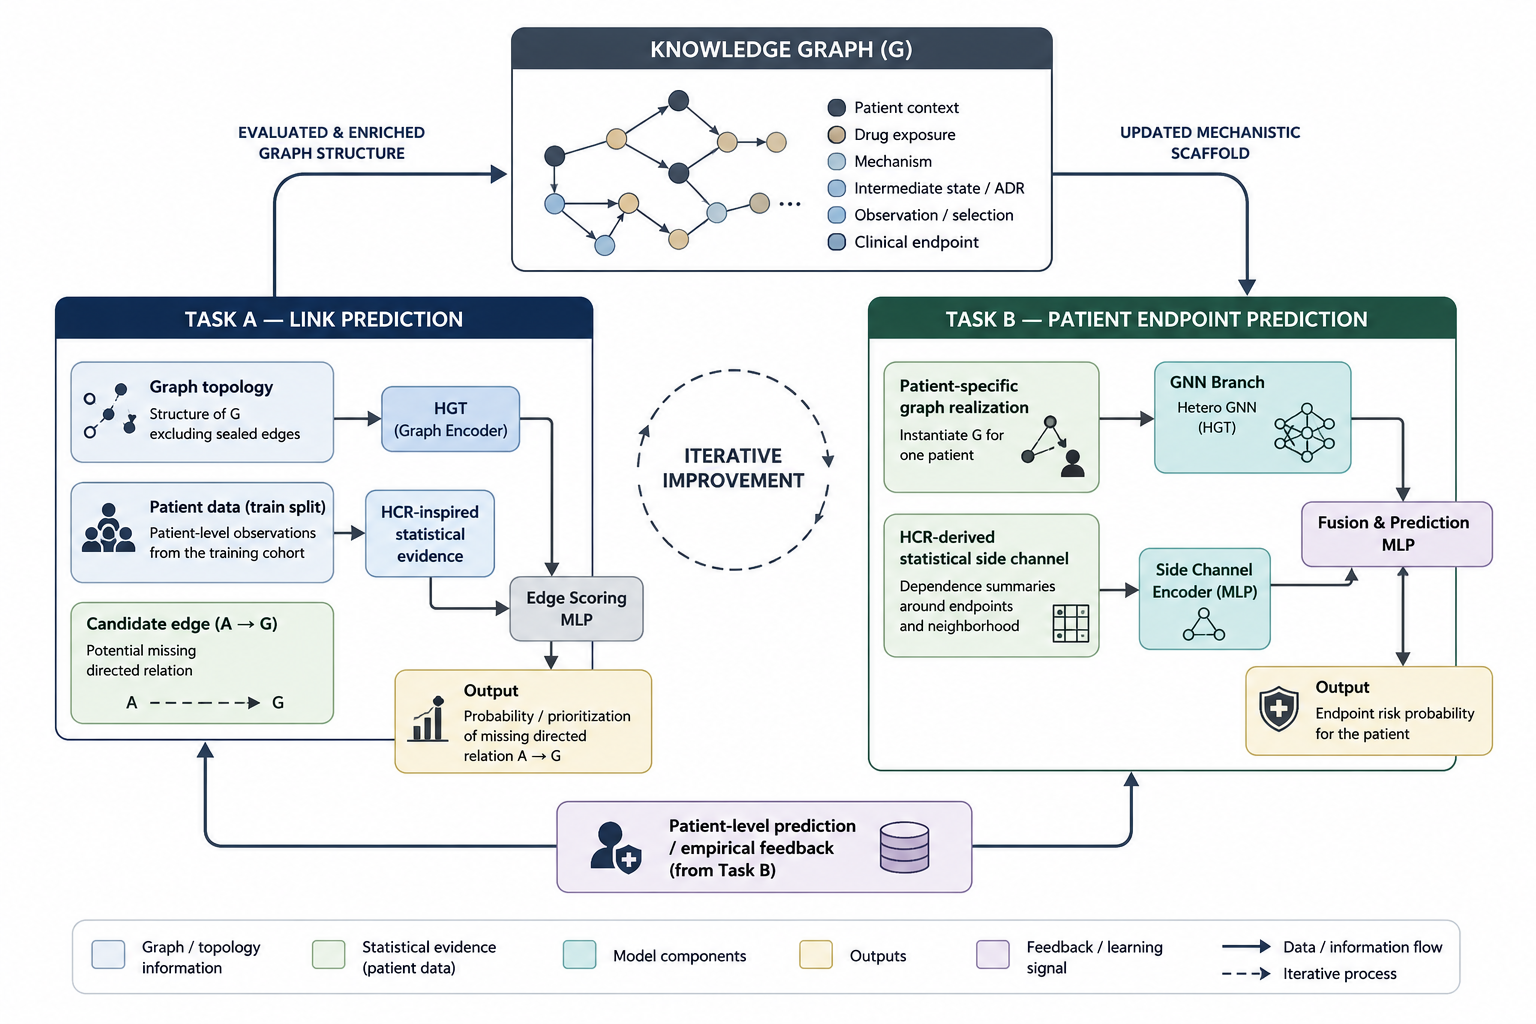
\includegraphics[width=0.92\textwidth,height=0.32\textheight,keepaspectratio]{fig_loop_task_a_b.png}
    \caption{Intended research direction: an iterative loop between Task~A
    (evaluation of graph relations) and Task~B (patient-level endpoint prediction).}
    \label{fig:loop}
    \label{fig:intro-task-loop}
\end{figure}
\chapter{Objectives and Contributions}
\label{ch:objectives}

The main objective of this thesis is to investigate how structured knowledge represented by a medical knowledge graph can be combined with statistical evidence derived from patient-level data.
The problem is studied through two complementary tasks: graph reconstruction and patient-level clinical endpoint prediction.

The specific contributions of the thesis are:

\paragraph{Task A. Directed link prediction.}
A method is developed for evaluating candidate directed relations in a heterogeneous pharmacotherapy 
graph by combining graph structure with explicit empirical evidence from patient-level data. 
The graph component, implemented with a Heterogeneous Graph Transformer (HGT), provides a 
topology-constrained representation of the candidate relation and its local typed context. 
The statistical component characterizes the geometry and strength of dependence observed in 
patient-level data using coefficients derived from Hierarchical Correlation Reconstruction (HCR), 
together with additional statistical descriptors. Both representations are then combined and passed 
to a common decoder for directed link prediction. The same principle is additionally examined using 
Last-FM, a corrected music recommendation benchmark represented as a user–artist interaction graph, 
which serves as a proxy task under a substantially different graph structure and ranking objective. 
This allows us to assess whether the value of combining structural and explicit empirical 
information is specific to the pharmacotherapy setting or persists after a substantial change 
of domain.

\paragraph{Task B. Patient-level endpoint prediction.}
A patient-specific prediction framework is developed in which the shared pharmacotherapy graph provides the structural representation and patient observations provide individual input information.
Several GNN architectures and graph depths are evaluated, including the effect of residual connections on deeper message passing.
The graph representation is further complemented with an HCR-derived statistical side-channel describing dependencies between endpoints and their direct or higher-order graph neighbourhood.
Different forms of this statistical branch, including pairwise, type-specific and higher-order representations, are compared.
The resulting models are evaluated separately for clinical endpoints using metrics appropriate for imbalanced outcomes, including AUROC, Average Precision (AP) and lift.

In both cases, graph-based representation learning and explicit statistical dependence are treated as complementary sources of information rather than as competing alternatives.

\chapter{Related Work}
\label{ch:related-work}

This chapter reviews the background that motivates combining structured knowledge graphs with explicit statistical dependence estimates:
biomedical knowledge graphs, graph neural networks for heterogeneous relational data, 
Hierarchical Correlation Reconstruction, and knowledge-aware recommendation with evaluation reliability.

\section{Knowledge Graphs in Biomedicine}
\label{sec:related-kg}

The term \emph{knowledge graph} (KG), though traceable to proposals from the
1970s, entered widespread use after Google's 2012 announcement of its
knowledge graph, built on resources such as DBpedia and Freebase
\cite{hogan2021knowledge}. Since then, the concept has been adopted far
beyond web search, as it provides an interlinked representation of
knowledge in a human- and machine-understandable
format~\cite{barrasa2023building}.

This growth has been particularly visible in biomedicine, where
KGs are used to integrate heterogeneous sources such as
drugs, genes, diseases, and mechanisms of action (the biochemical process by which a drug produces its effect) 
~\cite{maclean2021knowledge}.
In biomedical KGs, entities (nodes $V$) may represent drugs, diseases, genes,
proteins, mechanisms, patient characteristics, or clinical outcomes, while
edges ($E$) describe typed relationships (e.g.,
\emph{drug--treats--disease}, \emph{gene--associates--disease}).
Such graphs are naturally heterogeneous and admit the form~\cite{hu2020hgt}
\begin{equation}
\label{eq:hetero-graph}
\begin{gathered}
G = \bigl(V, E, \tau, \phi\bigr), \\[0.3em]
{\scriptstyle
\tau \colon V \longrightarrow \mathcal{T}_V \text{ and }
\phi \colon E \longrightarrow \mathcal{T}_E
}
\end{gathered}
\end{equation}

Within this domain, knowledge graphs support a wide range of tasks,
spanning drug-drug interaction prediction, drug development, 
and clinical decision support~\cite{cui2025hkgreview}.
Among these, clinical decision support centres on
patient-level data as a core, rather than drug- or trial-related data.
Graph-based approaches within this patient-centric
setting have been applied to different tasks such as clinical prediction tasks including
in-hospital mortality and readmission~\cite{jiang2024graphcare}, survival
analysis~\cite{tan2023gnnsurv}, and multimodal risk prediction from
electronic health records (EHR)~\cite{zitnik2024graphai}.

At this point it is important to note that such clinical prediction models
could pursue different aims, such as risk prediction or treatment effect estimation. 
Risk models
predict the probability of an outcome under the patient's observed
factual course of care, whereas treatment effect estimation asks a
counterfactual question: how would the outcome differ under an
alternative treatment decision~\cite{hoogland2021tutorial}. This distinction motivates
 the design of our knowledge graph, which is structured to reflect 
 intended causal relations between entities and patient trajectories in 
 relation to specific treatments (drugs) and patient characteristics.
The decision was motivated by Toonsi et al.~\cite{toonsi2025causal} who propose
causal
knowledge graphs as a means of addressing several shortcomings of the
standard modelling pipeline simultaneously. 
As KG's edges are
intended to encode causal, rather than purely associative, relations,
causal knowledge graphs are more robust to distribution
shift between clinics and better suited to reasoning under incomplete
documentation, while also allowing prior medical knowledge to support
downstream prediction tasks~\cite{cui2025hkgreview}. 

Such graphs could be dynamically constructed from empirical data.
Standard pipelines for constructing KG include a dedicated
step for completing missing relations between entities using graph
databases or link prediction models, typically applied to graphs
derived from literature and curated sources~\cite{cui2025hkgreview}. 

%This
%thesis revisits the same construction step applying link prediction 
%to reconstruct relations within graphs
%built from empirical data.

Taken together, these observations motivate two complementary tasks
studied in this thesis: reconstructing
knowledge graphs via empirical patient-level data, and predicting clinical outcomes
on the resulting structure via node classification. The
tasks are addressed by GNNs described in the following section.

\subsection{Graph Neural Networks}
\label{subsec:related-gnn}

Graph neural networks (GNNs) learn node representations by aggregating
information from neighbouring nodes through message passing
\cite{hamilton2017graphsage}.
After $K$ message-passing layers, the representation of a node can
incorporate information from its $K$-hop neighbourhood.
During training, every node is represented not only by its own features, as
in traditional neural networks, but also by the features of its neighbours.
Unlike earlier graph-embedding methods with fixed representations, GNNs
build node embeddings inductively through aggregation, so inference does not
require all nodes to be present during training.

Formally, the representation $h_v^{(K)}$ of node $v$ depends on the features
of all nodes within its $K$-hop neighbourhood.
At layer $k$,
\begin{equation}
\label{eq:related-mp}
\begin{gathered}
h_v^{(k)} = \text{UPDATE}\Bigl(h_v^{(k-1)},\ \text{AGGREGATE}\bigl(\{h_u^{(k-1)} : u \in \mathcal{N}(v)\}\bigr)\Bigr), \\[0.3em]
{\scriptstyle
\mathcal{N}(v) \text{ --- neighbourhood of node } v
}
\end{gathered}
\end{equation}
so that information from a node $u$ at graph distance $d$ from $v$ only
reaches $v$ once $K \geq d$.
Different GNN architectures mainly differ in how neighbouring information
and, on heterogeneous graphs, relation types are transformed and aggregated.
Several architectures relevant to this thesis are reviewed below.

\subsubsection{GraphSAGE}

GraphSAGE~\cite{hamilton2017graphsage} was introduced for inductive and
scalable representation learning on large graphs.
It instantiates the general message-passing scheme using one of three
aggregation functions---mean, LSTM, or pooling---so that the same learned
functions can later be applied to unseen nodes.
GraphSAGE concatenates a node's own representation with the aggregated
neighbour representation and L2-normalises the result after each layer.
In order to improve scalability, it samples a fixed number of neighbours per node.

\subsubsection{Relational Graph Convolutional Network}

Relational Graph Convolutional Networks (R-GCNs)
\cite{schlichtkrull2018rgcn} extend graph convolutional networks to
multi-relational graphs, in which edges represent different types of
relationships.
Unlike a standard GCN, which applies the same transformation to messages
from all neighbours, R-GCN applies a relation-specific transformation.

For a node $v$, the representation at layer $l+1$ is computed as
\begin{equation}
\label{eq:rgcn}
\begin{gathered}
h_v^{(l+1)} =
\sigma \left(
\sum_{r \in \mathcal{R}}
\sum_{u \in \mathcal{N}_r(v)}
\frac{1}{c_{v,r}}
W_r^{(l)} h_u^{(l)}
+
W_0^{(l)} h_v^{(l)}
\right), \\[0.4em]
{\scriptstyle
\mathcal{R}\text{ --- relation types},\ 
\mathcal{N}_r(v)\text{ --- neighbours of }v\text{ under }r,\ 
c_{v,r}\text{ --- normalisation}
} \\[0.15em]
{\scriptstyle
W_r^{(l)}\text{ --- relation-specific weights},\ 
W_0^{(l)}h_v^{(l)}\text{ --- self-loop},\ 
\sigma\text{ --- activation}
}
\end{gathered}
\end{equation}

When the number of relation types is large, assigning a separate full weight
matrix to each relation can lead to overfitting.
R-GCN therefore introduces basis decomposition, in which each
relation-specific matrix is expressed as a linear combination of $B$ shared
basis matrices:
\begin{equation}
\label{eq:rgcn-basis}
\begin{gathered}
W_r^{(l)} =
\sum_{b=1}^{B} a_{rb}^{(l)} V_b^{(l)}, \\[0.4em]
{\scriptstyle
V_b^{(l)}\in\mathbb{R}^{d_{\mathrm{out}}\times d_{\mathrm{in}}}\text{ --- shared basis},\ 
a_{rb}^{(l)}\text{ --- coefficient for relation }r
}
\end{gathered}
\end{equation}

\subsubsection{Transformer-based message passing}

%Attention-based GNNs learn the importance of neighbouring nodes rather than
%using a fixed aggregation rule \cite{velickovic2018graphattention}.
Transformer-based graph neural networks adapt the self-attention mechanism
from the Transformer architecture of Vaswani et al.~\cite{vaswani2017attention} to
graph-structured data.
For each node $i$, its input representation $\mathbf{h}_i$ is projected into
query, key, and value vectors:
\begin{equation}
\label{eq:transformer-qkv}
\begin{gathered}
\mathbf{q}_i = \mathbf{W}_{Q}\mathbf{h}_i, \qquad
\mathbf{k}_i = \mathbf{W}_{K}\mathbf{h}_i, \qquad
\mathbf{v}_i = \mathbf{W}_{V}\mathbf{h}_i, \\[0.4em]
{\scriptstyle
\mathbf{W}_{Q},\;\mathbf{W}_{K},\;\mathbf{W}_{V}\text{ --- learnable projection matrices}
}
\end{gathered}
\end{equation}
For an edge from source node $j$ to target node $i$, the attention
coefficient is
\begin{equation}
\begin{gathered}
e_{ij} =
\frac{\mathbf{q}_{i}^{\top}\mathbf{k}_{j}}{\sqrt{d_k}}, \\[0.4em]
{\scriptstyle
d_k\text{ --- dimensionality of the key vectors}
}
\end{gathered}
\end{equation}
The attention coefficients are normalised across all neighbours of the
target node using the softmax function:
\begin{equation}
\label{eq:transformer-softmax}
\begin{gathered}
\alpha_{ij} =
\frac{\exp(e_{ij})}
{\sum_{r \in \mathcal{N}(i)} \exp(e_{ir})}, \\[0.4em]
{\scriptstyle
\mathcal{N}(i)\text{ --- neighbourhood of target node }i
}
\end{gathered}
\end{equation}
The node's representation is updated by aggregating value projections of
its neighbours, weighted by the learned attention coefficients:
\begin{equation}
\begin{gathered}
\mathbf{h}'_i =
\sum_{j \in \mathcal{N}(i)}
\alpha_{ij}\mathbf{v}_{j}, \\[0.4em]
{\scriptstyle
\alpha_{ij}\text{ --- attention weight},\ 
\mathbf{v}_{j}\text{ --- value projection of neighbour }j
}
\end{gathered}
\end{equation}

To capture multiple complementary interaction patterns, graph Transformers
commonly use multi-head attention.
The output of head $m$ for node $i$ is:
\begin{equation}
\begin{gathered}
\mathbf{h}_i^{\prime(m)} =
\sum_{j \in \mathcal{N}(i)}
\alpha_{ij}^{(m)}\mathbf{v}_{j}^{(m)}, \\[0.4em]
{\scriptstyle
m\in\{1,\ldots,H\},\ 
\mathbf{W}_{Q}^{(m)},\;\mathbf{W}_{K}^{(m)},\;\mathbf{W}_{V}^{(m)}\text{ --- independent projections per head}
}
\end{gathered}
\end{equation}
The outputs of all $H$ heads are combined by concatenation or averaging.

All architectures mentioned above are homogeneous from nature, but can be applied to heterogeneous
graphs through an appropriate configuration of the \texttt{HeteroConv} layer in
PyTorch Geometric (PyG). \texttt{HeteroConv} is a generic wrapper that applies
a separately specified message-passing operator to each edge type, i.e., each
meta-relation between a source node type and a target node type~\cite{wojcik2026grafowe}.
This mechanism is used in Task B which allowed to experiment with different graph architectures 
on joined setting.


\subsubsection{Heterogeneous Graph Transformer}

In response to the demand for preserving heterogeneous structure during modelling, Hu et al.~\cite{hu2020hgt} 
proposed the Heterogeneous Graph Transformer (HGT).
For attention-based message passing on heterogeneous graphs, the
Heterogeneous Graph Transformer (HGT) makes attention scores and message
transformations dependent on the types of source and target nodes and on the
edge relation.
Unlike the \texttt{HeteroConv}-wrapped TransformerConv described above,
which instantiates a fully independent set of attention parameters for
each edge type and aggregates their outputs only after each layer has
been computed separately, HGT shares a single underlying attention
mechanism across all edge and node types, using type-specific projection
matrices. This allows HGT to learn
interactions across types directly, at a lower parameter cost as the
number of types grows~\cite{hu2020hgt}.

The HGT layer decomposes message passing
into three components: heterogeneous mutual attention, heterogeneous
message passing, and target-specific aggregation. Each component uses a
separate set of weight matrices for every combination of source node
type, edge type, and target node type -- referred to as a
\emph{meta relation} $(\tau_s, \phi(e), \tau_t)$.
%For an edge from source node $s$ to target node $t$, HGT represents its
%semantics as a meta-relation $(\tau_s, \phi(e), \tau_t)$, where $\tau_s$
%and $\tau_t$ denote the source and target node types and $\phi(e)$ denotes
%the edge type.
So that HGT extends the query, key, and value projections introduced in
Eq.~\eqref{eq:transformer-qkv} by conditioning each weight matrix on node
type: $\mathbf{W}_{Q}^{\tau_t}$, $\mathbf{W}_{K}^{\tau_s}$, and
$\mathbf{W}_{M}^{\tau_s}$ replace the shared $\mathbf{W}_{Q}$,
$\mathbf{W}_{K}$, and $\mathbf{W}_{V}$, so that
\begin{equation}
\mathbf{q}_t = \mathbf{W}_{Q}^{\tau_t}\mathbf{h}_t, \qquad
\mathbf{k}_s = \mathbf{W}_{K}^{\tau_s}\mathbf{h}_s, \qquad
\mathbf{m}_s = \mathbf{W}_{M}^{\tau_s}\mathbf{h}_s.
\end{equation}
The attention coefficient additionally depends on the edge type through a
relation-specific matrix $\mathbf{W}^{\phi(e)}_{\text{ATT}}$:
\begin{equation}
e_{ts} =
\frac{\left(\mathbf{q}_t^{\top}\mathbf{W}^{\phi(e)}_{\text{ATT}}\mathbf{k}_s\right)}
{\sqrt{d_k}},
\qquad
\alpha_{ts} = \frac{\exp(e_{ts})}{\sum_{r \in \mathcal{N}(t)} \exp(e_{tr})}.
\end{equation}
The message is similarly transformed by a relation-specific matrix
$\mathbf{W}^{\phi(e)}_{\text{MSG}}$ and aggregated across all neighbours
of $t$:
\begin{equation}
\label{eq:hgt-aggregation}
\mathbf{h}'_t =
\sum_{s \in \mathcal{N}(t)}
\alpha_{ts}\left(\mathbf{m}_s\mathbf{W}^{\phi(e)}_{\text{MSG}}\right)~\cite{hu2020hgt}.
\end{equation}
Relation-specific transformations affect both the attention
score and the transferred message, so that HGT assigns different
importance to neighbours based not only on their features, but also on
the semantic type of their connection to the target node.

As $\mathbf{h}'_t$ combines information from source nodes of
potentially different types and feature distributions, it is mapped back
into the target node's type-specific space via a target-type-dependent
projection, followed by a non-linear activation and a residual
connection to the previous layer:
\begin{equation}
\mathbf{h}''_t =
\mathbf{A}\text{-}\mathrm{Linear}_{\tau_t}
\left(\sigma\left(\mathbf{h}'_t\right)\right)
+ \mathbf{h}_t^{(l-1)}~\cite{hu2020hgt}.
\end{equation}

This capacity to differentiate neighbours by both node type and
relation semantics is particularly relevant to the knowledge graphs
built for the purpose of this thesis, where clinically distinct relation types --
such as drug--drug interactions versus drug--outcome relations -- 
 carry different predictive weight. 
HGT is the primary structural encoder in Task~A and proxy to Task~A, because typed
pharmacotherapy and collaborative-knowledge-graph relations require type-aware message
passing. 



% DropEdge (Rong et al., 2020) randomly removes a fraction of edges independently in every layer during training, slowing the rate of information mixing and acting as a structural regularizer.

% Jumping Knowledge (Xu et al., 2018) aggregates the outputs of all layers (via concatenation, cat, or elementwise max) rather than only the last one, letting a node fall back on a shallower, less-smoothed representation when the deepest layer has become uninformative.

% Weisfeiler-Lehman --- two nodes with identical initial features and structurally equivalent neighborhoods 
% cannot be assigned distinct representations by any number of convolutional layers.

% leave-one-out

\section{Statistical Dependence and Hierarchical Correlation Reconstruction}
\label{sec:related-hcr}
\label{subsec:hcr_def}

Empirical comparisons between graph-based and tabular models report
mixed results, with gains from graph structure often modest and
architecture-dependent~\cite{tabgraphs2024,zhu2025stroketh}. Rather than
resolving this solely through architecture search, this thesis follows
the Wide\,\&\,Deep paradigm~\cite{cheng2016wideanddeep,gao2021wdgnn}, in
which a linear or statistically-grounded branch complements a deep,
graph-based branch. The wide branch memorises direct, low-order
statistical dependencies that message passing may dilute through
neighbourhood aggregation, while the deep branch generalises through
learned relational representations.  
In this thesis, the wide branch is introduced using
Hierarchical Correlation Reconstruction (HCR) described in this section.

HCR, proposed by Jaros\l{}aw Duda, represents probability distributions and statistical dependencies through coefficients of an orthonormal basis expansion~\cite{duda2018hcr,duda2018hcr-ts,duda2020hcr-income,duda2023hcr-wolfram,duda2025hcr-mi}.
Lower-order coefficients describe broad dependence patterns; higher-order coefficients capture more complex departures from independence.

For variables $X$ and $Y$ with orthonormal bases $\{\phi_j^{(X)}\}$ and $\{\phi_k^{(Y)}\}$, empirical cross-dependence coefficients are
\begin{equation}
a_{jk}
=
\frac{1}{n}
\sum_{i=1}^{n}
\phi_j^{(X)}(X_i)\,
\phi_k^{(Y)}(Y_i).
\end{equation}
For a binary variable $B\in\{0,1\}$ with prevalence $p_B=P(B=1)$,
\begin{equation}
\phi_1(B)=\frac{B-p_B}{\sqrt{p_B(1-p_B)}},
\end{equation}
so the lowest-order coefficient $a_{11}$ is a standardized first-order dependence descriptor.
The same principle extends to other variable types via suitable marginal bases.

HCR has demonstrated practical value in domains requiring reliable,
interpretable estimates of conditional distributions instead of single
point predictions. In virtual screening for drug discovery, HCR-based
prediction of ADMET property distributions enables inexpensive
selection of compounds with properties nearly certain to fall within a
desired range, while automatically flagging predictions with high
uncertainty for manual review~\cite{szarek2022hcrmolecular}. In income
credibility assessment using Polish household budget survey data, HCR
produced more accurate proxies for low-income households than
conventional tax-record matching, showing its ability to model the
conditional distribution directly instead of relying on a single
regression estimate~\cite{duda2020hcr-income,brzezinski2022polishinequality}.

Based on those results, in this work HCR is used as a statistical representation of empirical and 
associative dependence to complement the GNN representation.
Causal direction and
mechanistic interpretation are instead supplied by the directed graph
schema itself built for the purpose of this thesis.
In general the term HCR denotes the orthonormal-basis coefficient construction, whereas this thesis
uses HCR-inspired representations -- larger task-specific vectors that 
combine those coefficients with additional descriptors.
In Task~A they describe the local dependency motif around a candidate edge, while in Task~B they supply 
an endpoint-neighbourhood evidence channel alongside the GNN representation.
The common principle is combining learned graph representations with explicit statistical 
dependence estimated from observations.

\chapter{Dataset}
\label{ch:dataset}

\section{Synthetic Pharmacotherapy Dataset}

The primary dataset used in this thesis is Synthetic Pharmacotherapy Graph v3, a controlled benchmark designed to connect a known mechanistic graph structure with patient-level empirical observations.
The dataset was constructed specifically to support both tasks investigated in the thesis: reconstruction of graph relations in Task~A and patient-level endpoint prediction in Task~B.
It consists of two complementary components: a directed pharmacotherapy graph and patient-level records generated from that graph.

The use of synthetic data provides access to a known reference graph and to the complete data-generating process.
This makes it possible to introduce controlled observational artefacts while preserving the underlying mechanistic structure.
The dataset should therefore be interpreted as methodological ground truth for model evaluation.
Graph coefficients, baseline probabilities and realised endpoint rates are simulation parameters and must not be interpreted as estimates of real clinical effects.

\section{Pharmacotherapy Knowledge Graph}

The graph was designed as a directed acyclic graph (DAG) representing pathways from patient characteristics and drug exposures, through physiological mechanisms and intermediate adverse states, to clinical outcomes.
Graph construction started from clinically relevant endpoints and proceeded backwards through their expected determinants and mechanistic pathways.

Domain knowledge in pharmacology was used to define and review the initial set of drug classes, risk factors, mechanisms and clinical endpoints.
Claude Fable~5 was used as an AI-assisted modelling tool to propose candidate mechanistic pathways, including drug--drug and drug--disease interaction structures.
Importantly, the model was used to support pathway drafting rather than to determine the final graph automatically.
Proposed relations were reviewed and could be accepted, rejected or modified before inclusion in the graph specification.

The graph was developed iteratively and subsequently audited for structural consistency.
The final v3 graph contains 155 nodes and 405 directed edges and is acyclic, with no duplicate nodes, duplicate edges or references to missing nodes.
The nodes are organised into six semantic categories:

\begin{table}[ht]
\centering
\caption{Node types in Synthetic Pharmacotherapy Graph v3.}
\label{tab:dataset-node-types}
\begin{tabular}{@{}llp{7.2cm}@{}}
\toprule
Node type & Number & Role \\
\midrule
\texttt{patient\_context} & 24 & demographics, comorbidities and other patient-level characteristics \\
\texttt{drug\_exposure} & 29 & exposure to drug classes \\
\texttt{mechanism} & 49 & physiological mechanisms, interaction gates and drug-load variables \\
\texttt{adr\_or\_intermediate\_state} & 28 & intermediate adverse or physiological states \\
\texttt{observation\_or\_selection} & 12 & testing, documentation and selection processes \\
\texttt{clinical\_endpoint} & 13 & target clinical outcomes \\
\bottomrule
\end{tabular}
\end{table}

These categories distinguish patient context, treatment, biological mechanisms, intermediate consequences, observation processes and final clinical events.

\begin{figure}[htbp]
\centering
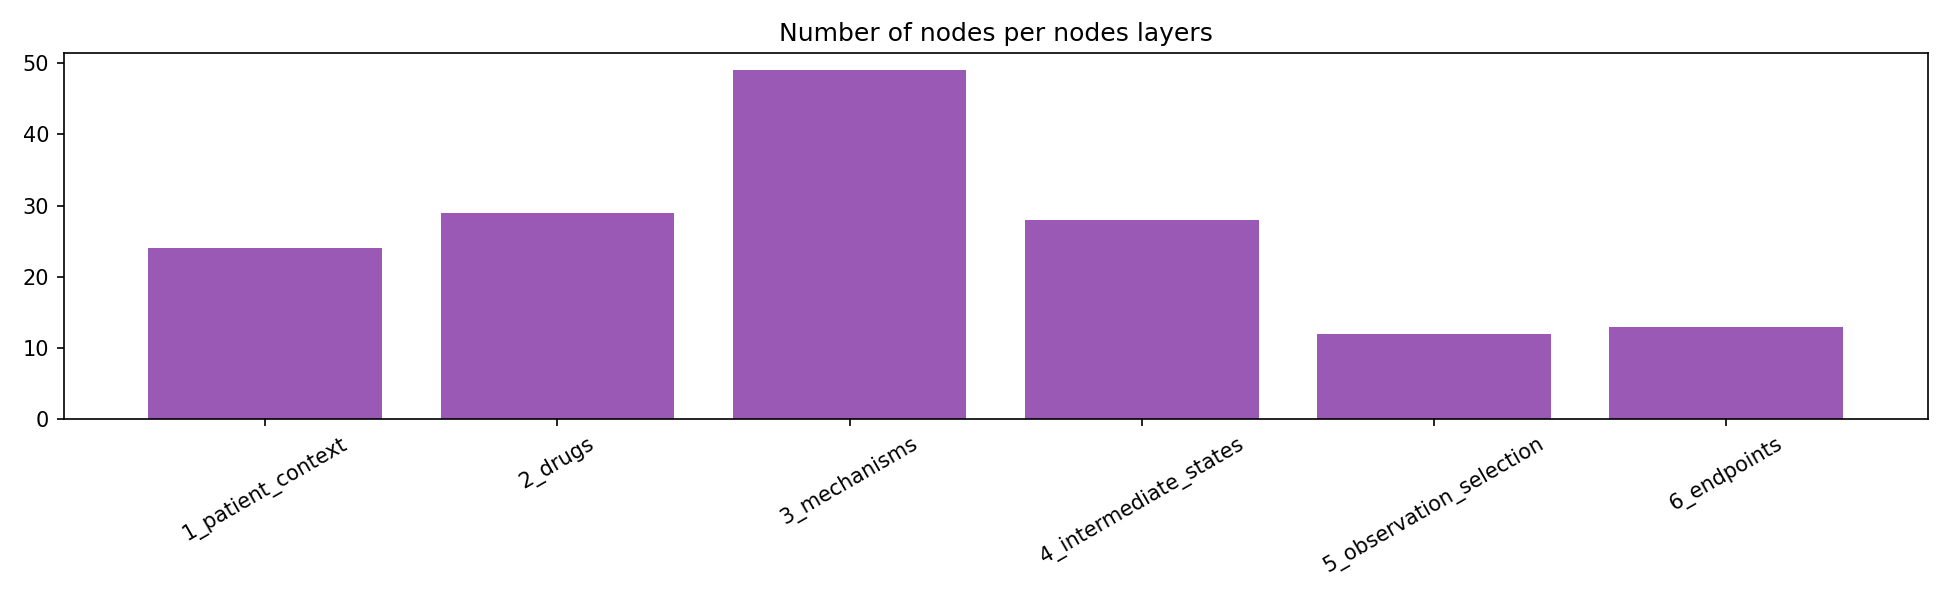
\includegraphics[width=\textwidth]{01_node_counts_by_type_and_layer.png}
\caption{Number of nodes in each semantic layer of Synthetic Pharmacotherapy Graph~v3.}
\label{fig:dataset-node-counts}
\end{figure}

Directed edges represent different semantic relationships, including background risk, treatment assignment, drug-to-mechanism effects, mechanistic progression, adverse-state progression, observation processes, and drug--drug or drug--disease interactions.
Edge attributes include the simulated magnitude and sign of an effect, which are subsequently used by the patient generator.

The graph contains 13 clinical endpoints regarded as points of clinical state requiring intervention:
AKI, DILI, Depression, Falls, Delirium, GI bleeding, Hyponatremia, Hyperkalemia, QT arrhythmia, Hospitalization, Serotonin syndrome, Rhabdomyolysis, and Lactic acidosis.

\begin{figure}[htbp]
\centering
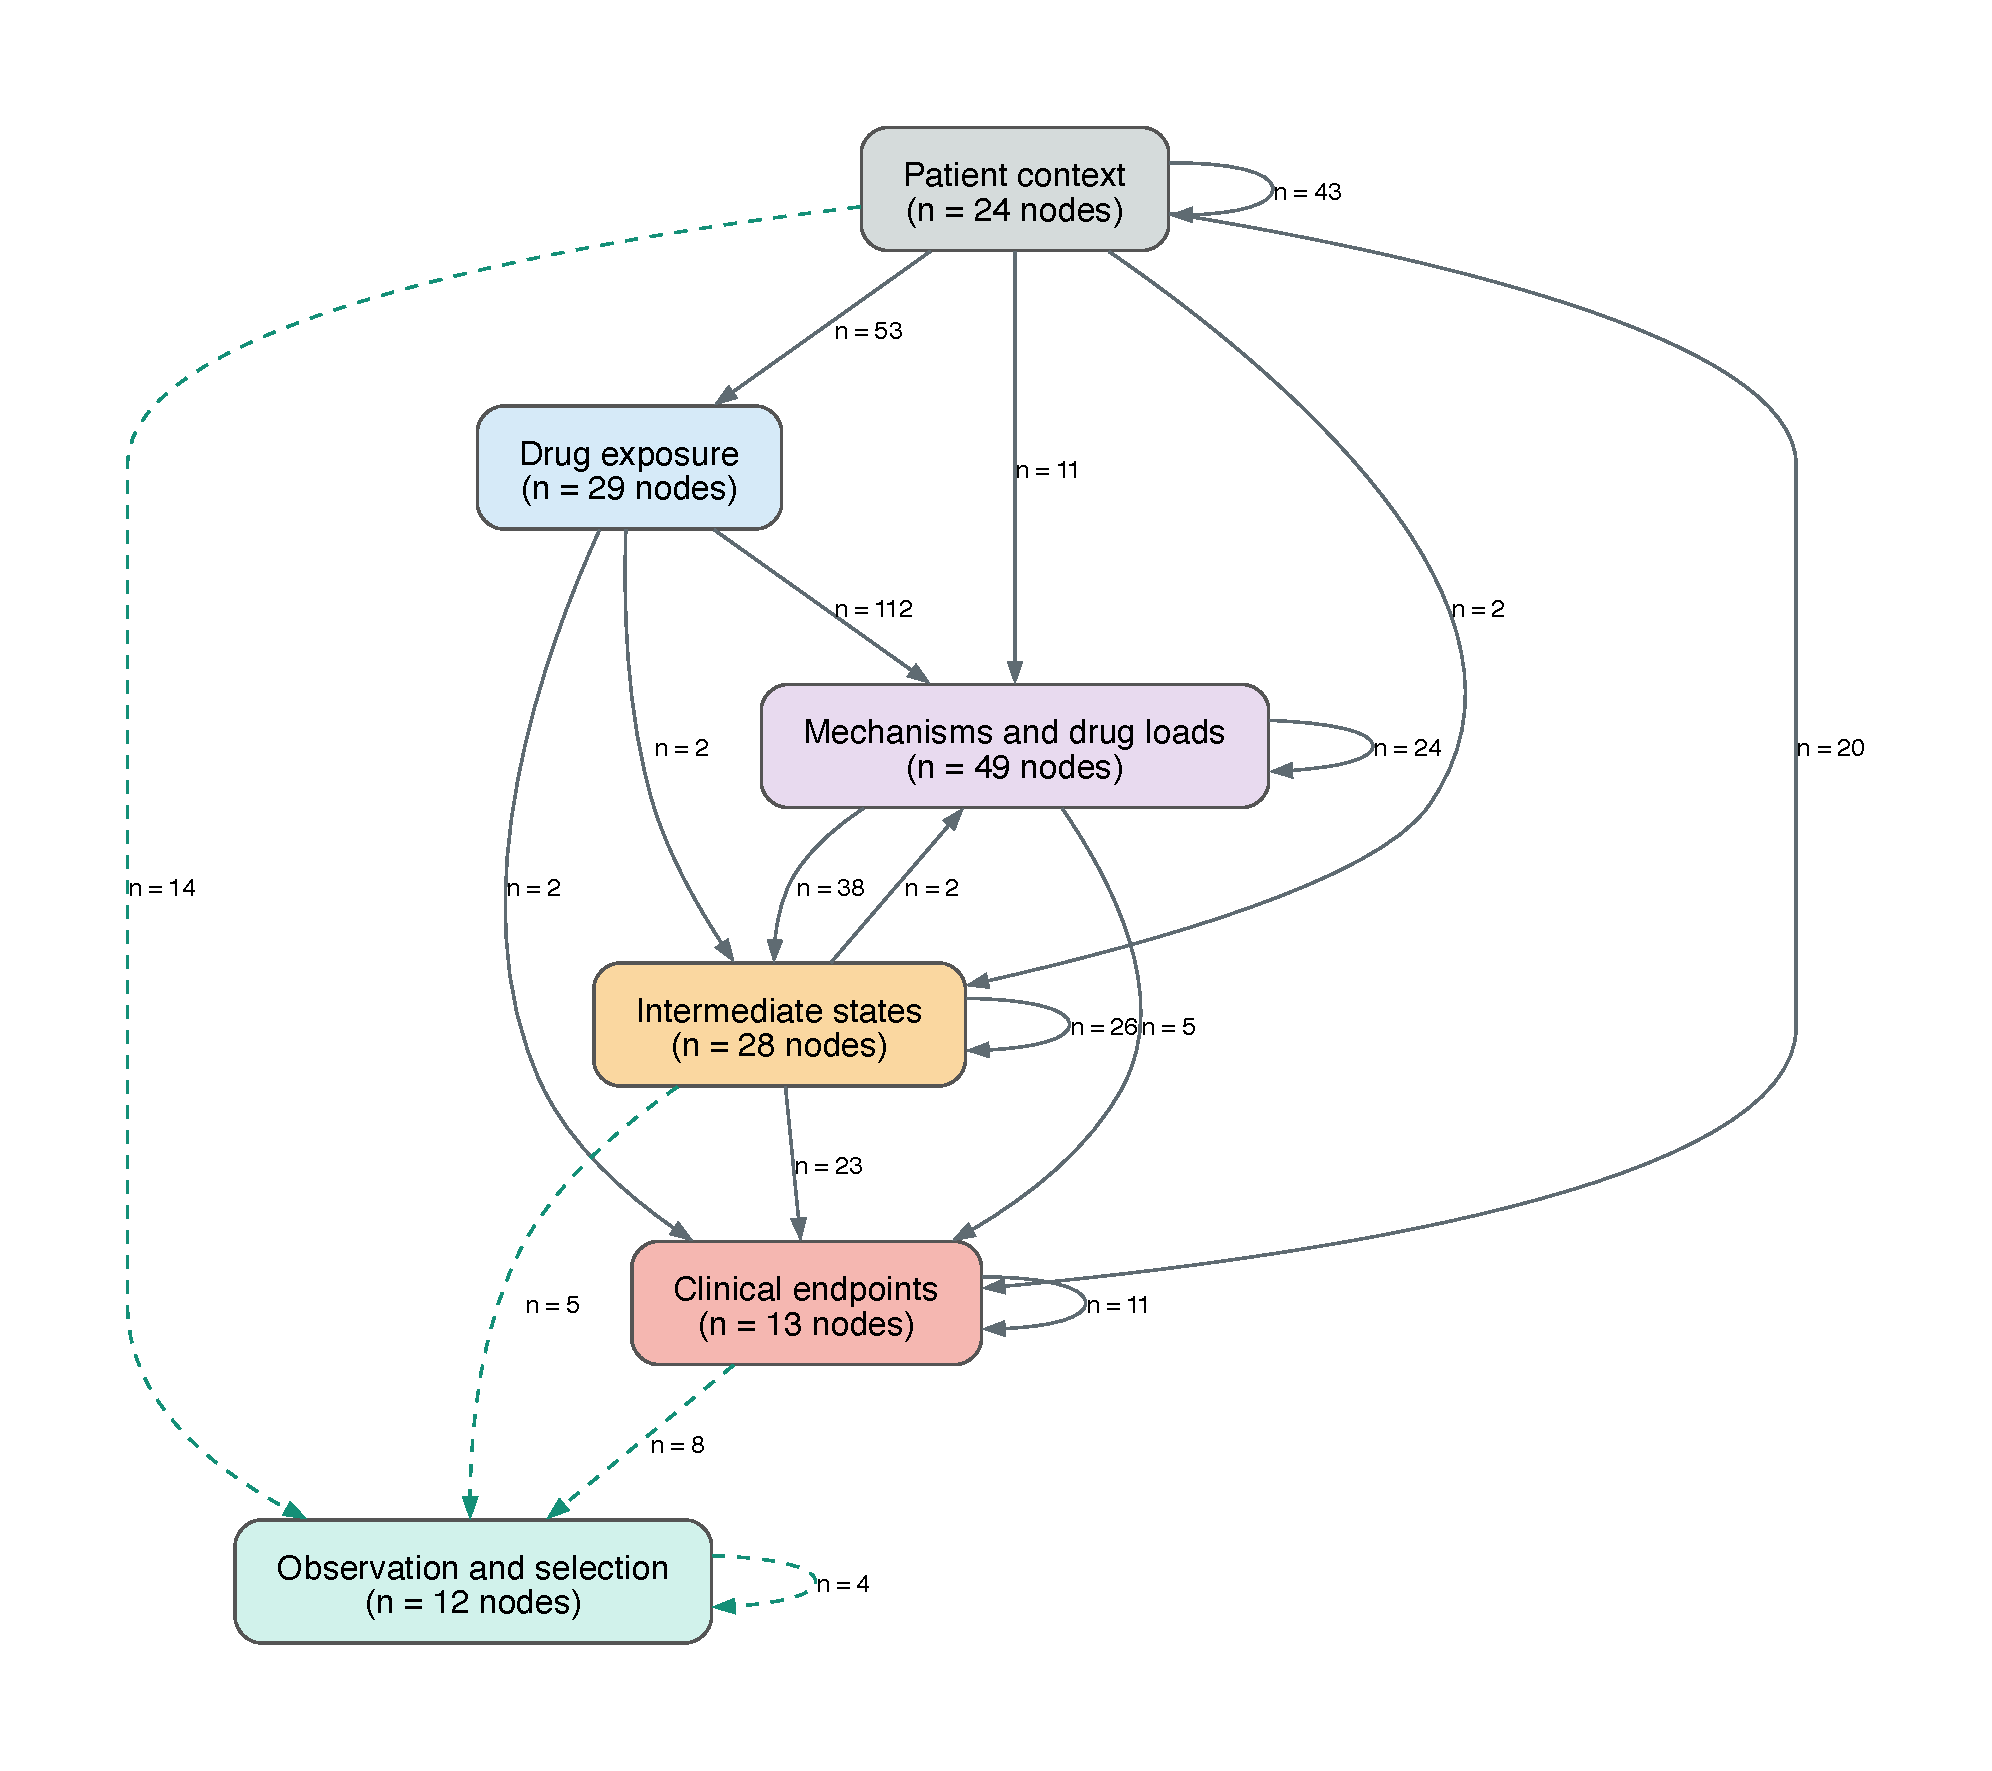
\includegraphics[width=\textwidth]{causal_dag_type_overview.pdf}
\caption{Overview of the synthetic pharmacotherapy DAG with node colours by semantic type.}
\label{fig:dag-overview}
\end{figure}

\begin{figure}[htbp]
\centering
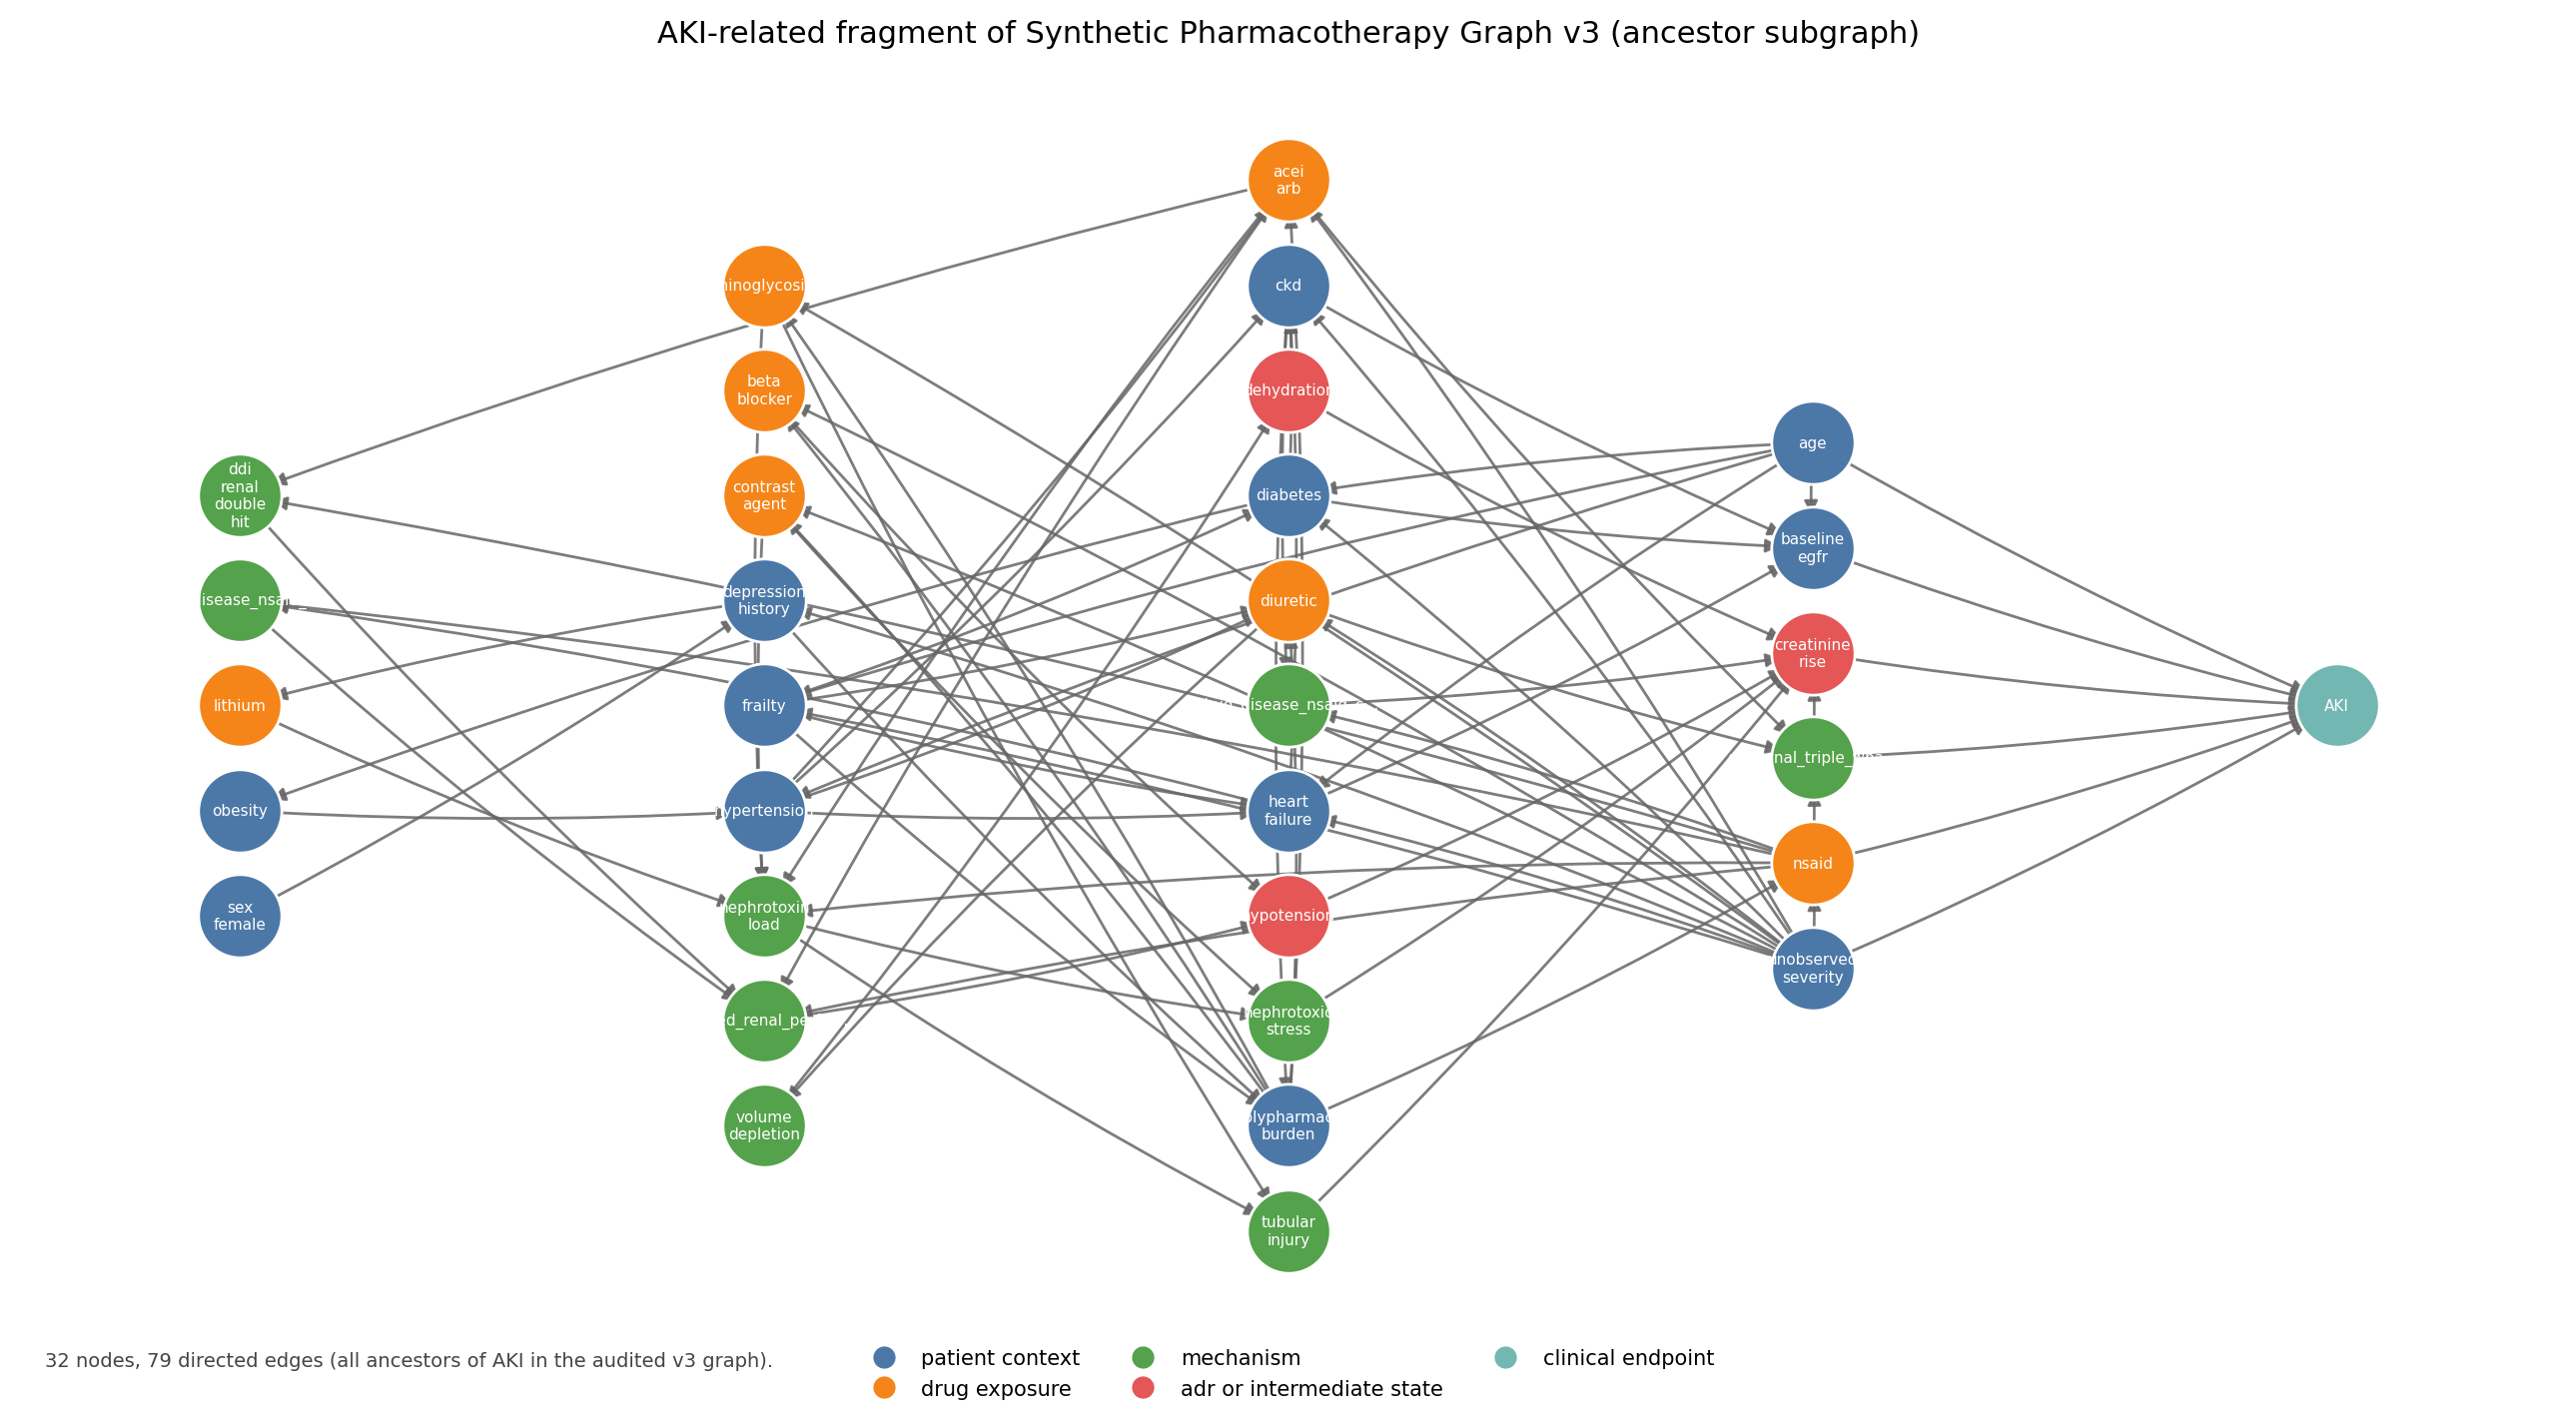
\includegraphics[width=\textwidth]{fig_aki_kg_fragment_networkx.png}
\caption{AKI-related fragment of the Synthetic Pharmacotherapy Graph~v3: all audited ancestors of the AKI endpoint ($32$ nodes / $79$ edges), drawn with NetworkX.
Node colours follow the v3 ontology (patient context, drug exposure, mechanism, ADR/intermediate state, clinical endpoint).
The full graph is larger; this excerpt is for orientation.}
\label{fig:aki-kg-fragment}
\end{figure}

\section{Patient-Level Data Generation}

The graph defines a common mechanistic structure, whereas the patient table represents individual realisations of that structure.
For each simulated patient, values are generated for the graph variables in topological order.
Patient-context variables are generated first, followed by drug exposures, mechanisms, intermediate states and finally clinical endpoints.
As a result, a parent variable is always realised before a downstream child variable is generated.

Most stochastic binary nodes are generated using an additive logistic model.
For node $i$,
\begin{equation}
\eta_i
=
\mathrm{logit}(p_i^{0})
+
\sum_{j\in\mathrm{parents}(i)}
s_{ij}\,w_{ij}\,x_j,
\end{equation}
followed by
\begin{equation}
x_i\sim\mathrm{Bernoulli}\!\left(\sigma(\eta_i)\right),
\end{equation}
where $p_i^{0}$ denotes the baseline probability of the node, $x_j$ is the realised value of parent $j$, and $w_{ij}$ and $s_{ij}$ denote the simulated effect magnitude and sign associated with the edge $j\to i$.
Count and continuous parents are standardised before entering the additive predictor.

Not all variables are stochastic.
The generator also contains deterministic quantities representing clinically meaningful combinations such as drug loads, drug--drug interaction gates, drug--disease interactions and cumulative adverse-event burden.
For example, some interaction variables are activated only when several required drug exposures are simultaneously present.

The dataset additionally separates an underlying clinical state from whether that state is observed or documented.
For example,
\begin{equation}
\texttt{elevated\_creatinine\_recorded}
=
\texttt{creatinine\_rise}
\times
\texttt{creatinine\_tested}.
\end{equation}
A true creatinine rise can therefore occur without being present in the recorded representation if testing is not performed.
This distinction allows documentation and selection artefacts to be introduced without changing the underlying mechanistic graph.

The clean dataset contains 20{,}000 simulated patients.
Each row corresponds to one patient, while graph nodes correspond to patient-level variables.
The 155 graph variables include binary, count and continuous values; the dataset additionally contains technical identifiers such as \texttt{patient\_id} and \texttt{hospital\_id}.

\section{Observational Scenarios}

Six scenarios were generated from the same underlying pharmacotherapy graph.
They were designed to test whether the models remain robust when the patient-level evidence is affected by different observational artefacts.

\begin{table}[ht]
\centering
\caption{Observational scenarios derived from the same pharmacotherapy graph.}
\label{tab:dataset-scenarios}
\begin{tabularx}{\textwidth}{@{}lXr@{}}
\toprule
Scenario & Purpose & Patients \\
\midrule
\texttt{clean} & reference setting with complete generated information & 20{,}000 \\
\texttt{hidden\_confounder} & latent severity remains active in generation but is withheld from observed data & 20{,}000 \\
\texttt{selection\_bias} & cohort restricted according to healthcare-contact and testing variables & 14{,}062 \\
\texttt{no\_overlap} & selected treatment exposures become rare in particular patient subgroups & 20{,}000 \\
\texttt{noisy\_documentation} & imperfect recording with false-negative and false-positive documentation & 20{,}000 \\
\texttt{multihospital} & heterogeneous treatment and documentation processes across four simulated hospitals & 20{,}000 \\
\bottomrule
\end{tabularx}
\end{table}

The scenarios differ in the observability and distribution of patient-level data, while the underlying graph semantics are preserved.
Importantly, the \texttt{selection\_bias} dataset is an intentional subset of the original population and therefore contains 14{,}062 patients.

\section{Patient Splits and Use Across Tasks}

Patients are divided into training, validation and test sets in proportions of 70\%, 15\% and 15\%.
For the clean cohort, this corresponds to 14{,}000 training patients, 3{,}000 validation patients and 3{,}000 test patients.
The split is defined at the patient level and reused across the alternative scenarios to maintain comparable patient partitions whenever possible.

The two tasks use this split differently.
In Task~A, patient records are not themselves the prediction instances: the training-patient partition is used to estimate node-level statistics and pairwise dependence measures, while the prediction instances are candidate graph edges.
The Task~A candidate inventory, negative-sampling rule and edge-level split are defined in Chapter~\ref{ch:taskA-rozwiazanie}.

In Task~B, the patient split itself defines the training, validation and test populations.
Each patient contributes individual node values and clinical endpoint labels, while the graph provides the common mechanistic scaffold.

All statistics derived from patient-level data are computed using the appropriate training partition only.
For Task~B, endpoint values, post-event or definitional intermediates, and other variables unavailable at the intended prediction point are excluded from predictive inputs.


\chapter{Task A. Directed Link Prediction on the Synthetic Pharmacotherapy Graph}
\label{ch:taskA-rozwiazanie}
\label{ch:taskA-ewaluacja}
\label{ch:taskA-benchmark}

Task~A asks whether directed link prediction on a heterogeneous pharmacotherapy graph improves when a learned structural representation is combined with an explicit statistical description of patient-level dependence around each candidate edge.
The structural branch encodes training topology; the statistical branch encodes empirical dependence estimated from training patients; a shared decoder fuses both sources into an edge score.

\section{Problem Formulation}
\label{sec:taskA-problem}

We address directed link prediction among observable nodes of the Synthetic Pharmacotherapy Graph~v3 (Chapter~\ref{ch:dataset}).
For a candidate directed edge $A\to G$, the model produces a score
\begin{equation}
\label{eq:taskA-score}
s_{AG}=f_{\theta}(A,G;G_{\mathrm{train}},X_{\mathrm{train}}),
\end{equation}
where $G_{\mathrm{train}}$ is the message-passing graph available during training and $X_{\mathrm{train}}$ denotes the training-patient observations used to construct node features and pairwise statistical descriptors.
The score is transformed through the sigmoid function,
\begin{equation}
\label{eq:taskA-objective}
\hat{p}_{AG}=\sigma(s_{AG}),
\end{equation}
and the resulting value is used in the binary edge-classification objective.

A positive label indicates that the directed relation is present in the audited graph, whereas a negative label denotes a type-allowed non-edge.
The prediction is based on two complementary sources of evidence:
\begin{itemize}
\item \emph{graph structure}: the typed neighbourhood of $A$ and $G$ represented in $G_{\mathrm{train}}$;
\item \emph{patient-derived statistical evidence}: empirical dependence patterns estimated from training patients for the local motif surrounding the candidate edge.
\end{itemize}
Directionality is determined by the ordered candidate definition and the graph schema, while the pairwise dependence coefficients provide statistical evidence about the variables involved in the candidate relation.

\section{Task-Specific Data Preparation}
\label{sec:taskA-data}

The shared graph and patient scenarios are defined in Chapter~\ref{ch:dataset}.
This section specifies how that resource is turned into prediction instances, a message-passing graph, and node features for Task~A.
The candidate edge inventory is held fixed across observational scenarios, so scenario differences arise from changes in patient-level observability rather than from changes in which edges are scored.

\subsection{Candidate edges and splits}
\label{sec:taskA-candidates}

After restricting the audited graph to observable nodes, the candidate set contains $366$ positive directed edges and $1{,}098$ negatives ($r_{\mathrm{neg}}=3$), for $1{,}464$ candidates in total.
Negatives are drawn from non-edges that satisfy
\begin{equation}
\label{eq:taskA-neg-conditions}
u\neq v,\qquad (u,v)\notin E^{+},\qquad \bigl(\mathrm{type}(u),\mathrm{type}(v)\bigr)\in T_{\mathrm{allowed}},
\end{equation}
rather than from a uniform draw over all ordered node pairs.

Candidates are split independently of the patient split, at edge level, into train/validation/test partitions with proportions $70/15/15$, stratified by the binary edge label.
This yields $256/55/55$ positives and $768/165/165$ negatives.
Patient records are not prediction instances: the training-patient partition is used only to estimate node statistics and pairwise dependence, while labels are attached to candidate edges.

\subsection{Message-passing graph}
\label{sec:taskA-mp-graph}

The HGT encoder operates on a heterogeneous training graph $G_{\mathrm{train}}$ that is smaller than the full audited graph.
Only observable nodes enter the encoder; latent generator nodes are excluded.
Node types and relation names follow the audited v3 ontology (Chapter~\ref{ch:dataset}).

For each positive training relation $u\xrightarrow{r}v$, an auxiliary reverse relation $v\xrightarrow{r^{-1}}u$ is added for message passing.
Reverse relations have distinct identities and enable bidirectional information flow without implying that the underlying mechanistic relation is reversible.

Message passing uses only positive training edges from the candidate set.
Validation positives, test positives, and all negative candidates are excluded from $G_{\mathrm{train}}$.
Held-out candidates are scored by referencing their endpoints in the node embedding table; they are never inserted as edges into $G_{\mathrm{train}}$.

\subsection{Node features}
\label{sec:taskA-node-feats}

Each observable node $v$ receives a three-dimensional empirical feature vector computed from training patients only,
\begin{equation}
\label{eq:taskA-node-x}
x_v=
\bigl[
\mu^{\mathrm{train}}_v,\;
\sigma^{\mathrm{train}}_v,\;
m^{\mathrm{train}}_v
\bigr],
\end{equation}
where $\mu^{\mathrm{train}}_v$ and $\sigma^{\mathrm{train}}_v$ are the train-patient mean and standard deviation of $v$, and $m^{\mathrm{train}}_v$ is the train missingness rate.
Identity embeddings are not used.
Before message passing, each node type is projected independently,
\begin{equation}
\label{eq:taskA-input-proj}
h_v^{(0)}=\mathrm{Dropout}\!\bigl(
\mathrm{ReLU}\bigl(
\mathrm{LayerNorm}(W_{\mathrm{type}(v)}\,x_v)
\bigr)\bigr),
\end{equation}
with $W_{\mathrm{type}(v)}:\mathbb{R}^{3}\to\mathbb{R}^{d}$.
Input statistics are fixed after preprocessing; projection and convolution weights are learned.

\section{Model Architecture}
\label{sec:taskA-arch}

\subsection{Architecture Overview}
\label{sec:taskA-arch-overview}

Figure~\ref{fig:taskA-arch-overview} summarizes the full model.
The structural branch maps $G_{\mathrm{train}}$ through HGT to a graph pair representation $g_{\mathrm{graph}}$.
The statistical branch maps the local $AZ$/$AG$/$ZG$ motif through role-specific encoders to $g_{\mathrm{stat}}$.
Concatenation and a shallow decoder produce the edge logit.

\begin{figure}[htbp]
\centering
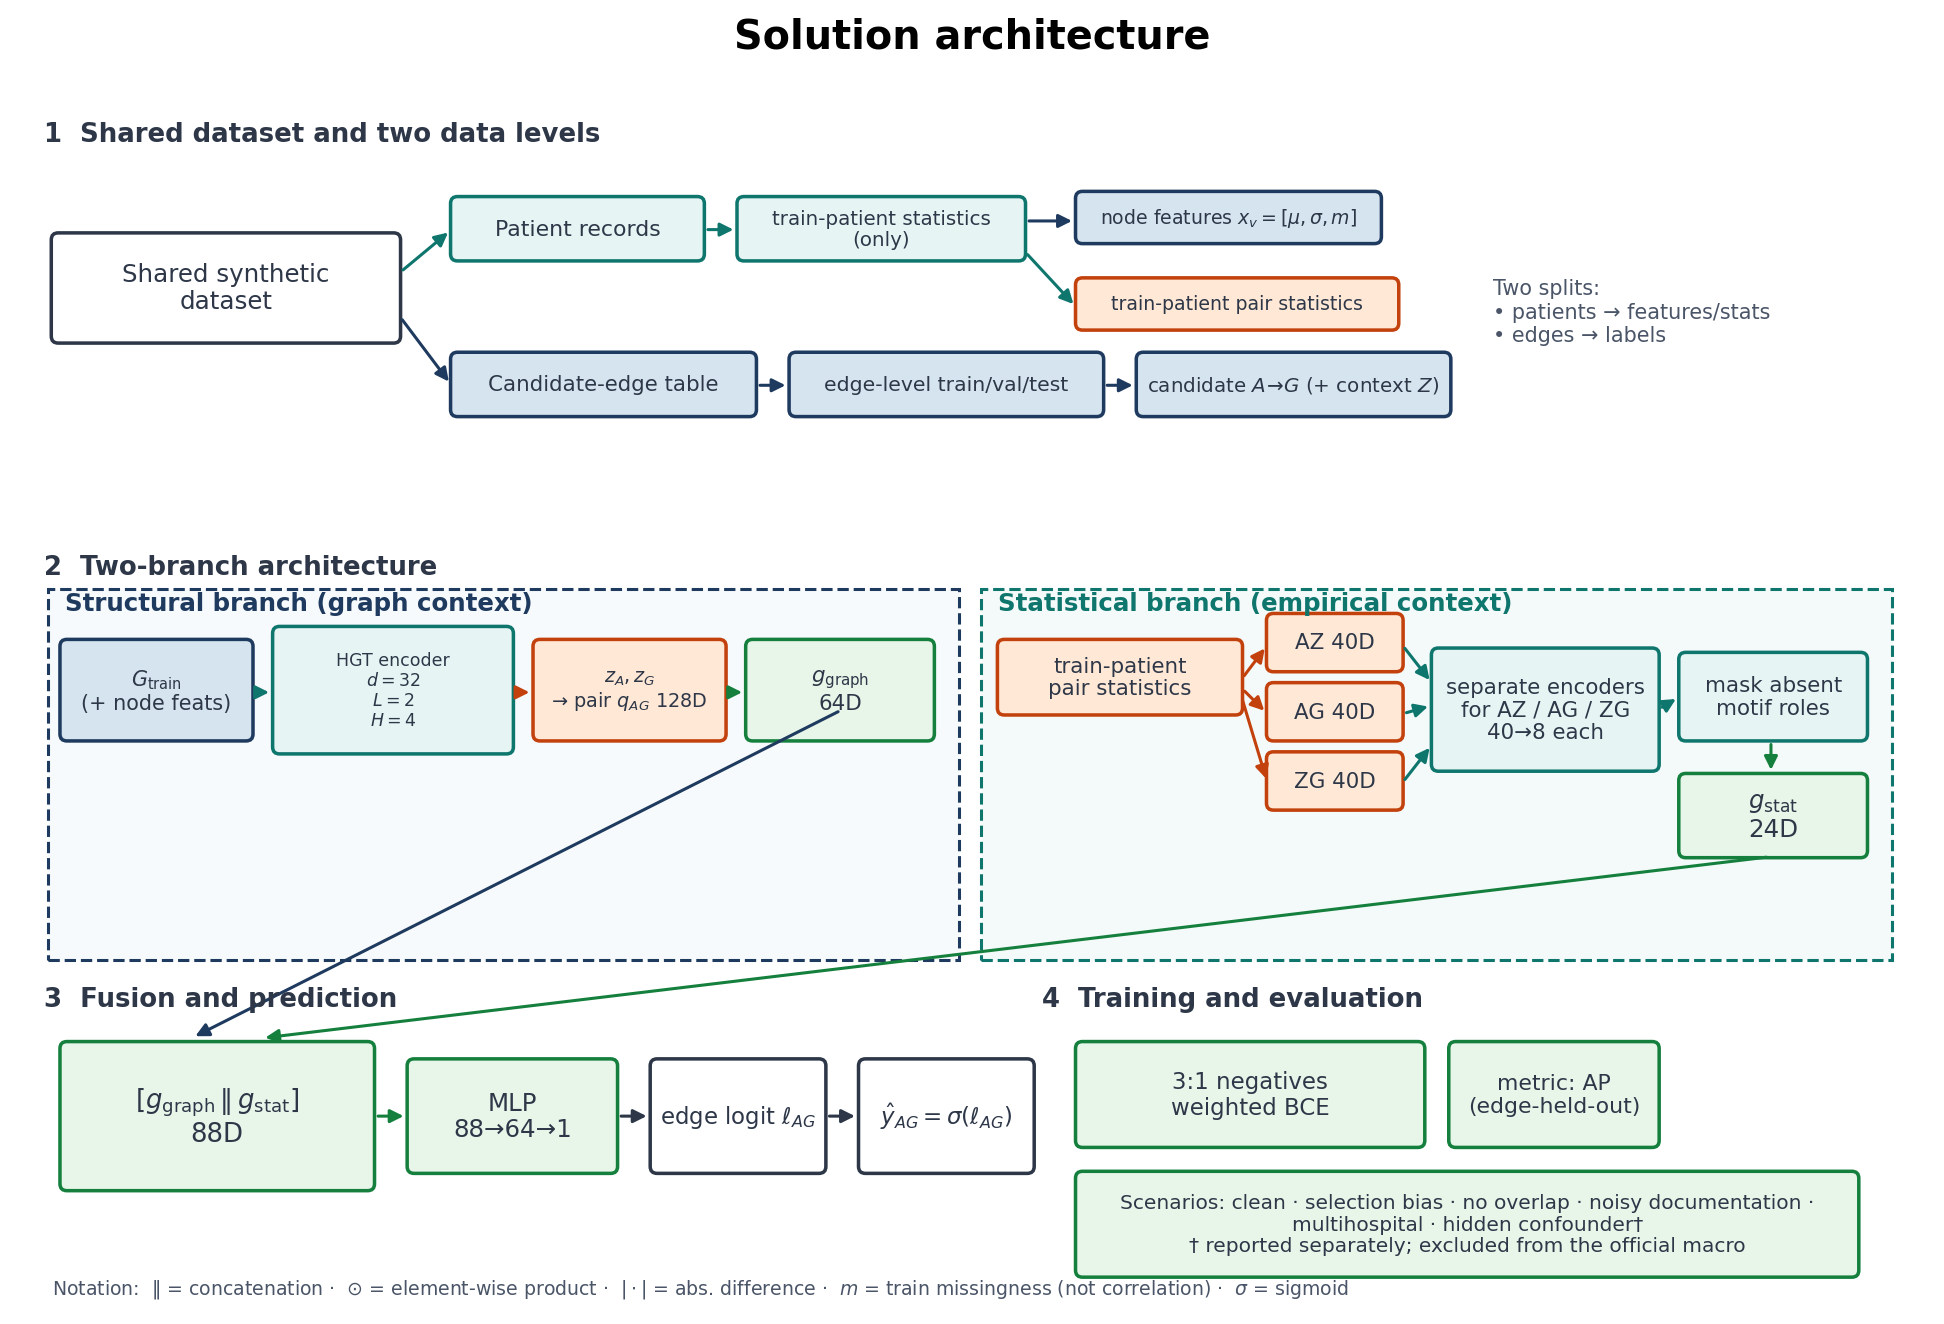
\includegraphics[width=\textwidth]{fig_taskA_arch_simplified.png}
\caption{Solution architecture for Task~A.
Patient records yield train-only node features $x_v=[\mu,\sigma,m]$ and pair statistics; candidate edges are split independently at edge level.
The structural branch maps $G_{\mathrm{train}}$ through HGT to $g_{\mathrm{graph}}\in\mathbb{R}^{64}$; the statistical branch encodes roles $AZ$/$AG$/$ZG$ with separate encoders and masks absent roles to $g_{\mathrm{stat}}\in\mathbb{R}^{24}$; fusion yields an edge logit.}
\label{fig:taskA-arch-overview}
\end{figure}

\subsection{Structural Branch}
\label{sec:taskA-hgt}

The graph encoder is a Heterogeneous Graph Transformer~\cite{hu2020hgt} with
\begin{equation}
\label{eq:taskA-hgt-hparams}
d=32,\qquad L=2,\qquad H=4,
\end{equation}
dropout $0.25$, LeakyReLU activations, and a residual connection with LayerNorm after each convolution layer.
These residual links are standard skip connections inside the encoder; they are not studied as an anti-oversmoothing intervention.

After $L$ layers, each observable node has an embedding $z_v\in\mathbb{R}^{32}$.
For candidate $A\to G$, the ordered pair representation is
\begin{equation}
\label{eq:taskA-qag}
q_{AG}=\bigl[z_{A}\parallel z_{G}\parallel z_{A}\odot z_{G}\parallel \lvert z_{A}-z_{G}\rvert\bigr]
\in\mathbb{R}^{128}.
\end{equation}
An MLP graph branch ($128\to 128\to 64$ with GELU and LayerNorm) compresses $q_{AG}$ to
\begin{equation}
g_{\mathrm{graph}}\in\mathbb{R}^{64}.
\end{equation}

\subsection{Statistical Evidence Branch}
\label{sec:taskA-hcr}

The general Hierarchical Correlation Reconstruction (HCR) formulation is stated in Chapter~\ref{ch:related-work}.
Task~A uses an HCR-inspired fixed-width pair vector so that binary, count, continuous and mixed pairs share one downstream interface.
HCR coefficients quantify empirical dependence; they do not identify causal direction.

For an ordered pair $(U,V)$, let $I_{UV}$ be the set of training patients with both variables observed and $n=|I_{UV}|$.
Type-specific orthonormal bases $\{\phi^{(U)}_{j}\}$ and $\{\phi^{(V)}_{k}\}$ yield coefficients
\begin{equation}
\label{eq:taskA-ajk}
a_{jk}
=
\frac{1}{n}
\sum_{i\in I_{UV}}
\phi^{(U)}_{j}(U_i)\,
\phi^{(V)}_{k}(V_i),
\end{equation}
zero-padded to a $4\times 4$ matrix and stored in the first $16$ dimensions of
\begin{equation}
\label{eq:taskA-h40}
h(U,V)\in\mathbb{R}^{40}.
\end{equation}
A binary variable contributes one non-constant contrast; continuous and jittered count variables may contribute up to four low-order basis functions, so the active block ranges from $1\times 1$ (binary--binary) to $4\times 4$.

The remaining dimensions summarize dependence magnitude and complexity, marginal context, joint activity and rarity, estimability, and variable type (Table~\ref{tab:taskA-hcr40}).
All quantities are fitted on training patients only.
An estimability indicator distinguishes unsupported pairs (coefficients zeroed) from genuine near-zero dependence.
Most components are intrinsically bounded or constructed in standardized bases; LayerNorm is applied inside the nonlinear pair encoder.
Complete formula-level definitions of the type-specific bases and all $40$ vector components are provided in Appendix~\ref{app:hcr-details}.

\begin{table}[!ht]
\centering
\footnotesize
\setlength{\tabcolsep}{4pt}
\caption{Grouped composition of the $40$-dimensional HCR-inspired pair representation.}
\label{tab:taskA-hcr40}
\begin{tabular}{@{}lcl@{}}
\toprule
Block & Dim.\ & Purpose \\
\midrule
HCR-inspired coefficients & $16$ & padded dependence-structure matrix $A_{\mathrm{pad}}$ \\
Dependence summaries & $4$ & magnitude and complexity of retained coefficients \\
Marginal context & $8$ & type-dependent descriptors of $U$ and $V$ \\
Joint activity / rarity & $4$ & co-activation enrichment and rarity \\
Support & $2$ & complete-case fraction and estimability flag \\
Variable types & $6$ & one-hot types of $U$ and $V$ \\
\bottomrule
\end{tabular}
\end{table}

For binary--binary pairs, signed Pearson $\phi$ is the natural first-order dependence coefficient and corresponds to the lowest-order HCR contrast; richer blocks retain higher-order structure that a single scalar association cannot express.

\subsection{Fusion and Prediction}
\label{sec:taskA-fusion}

For each candidate $A\to G$, a local context node $Z$ defines three ordered roles $AZ$, $AG$ and $ZG$ (source--context, candidate, context--target).
The same $40$-dimensional construction is applied to each role, yielding a raw motif of $120$ dimensions.
Each role is mapped by an independent MLP encoder
\begin{equation}
\label{eq:taskA-fr}
f_{r}:\mathbb{R}^{40}\to\mathbb{R}^{16}\to\mathbb{R}^{8},
\end{equation}
followed by a hard role gate
\begin{equation}
\label{eq:taskA-role-gate}
e_{r}=m_{r}\,f_{r}(h_{r}),\qquad m_{r}\in\{0,1\},
\end{equation}
so that absent roles (especially missing $Z$) contribute exactly zero.
The statistical branch output is
\begin{equation}
\label{eq:taskA-gstat}
g_{\mathrm{stat}}=[e_{AZ}\parallel e_{AG}\parallel e_{ZG}]\in\mathbb{R}^{24}.
\end{equation}

\begin{figure}[!ht]
\centering
\resizebox{0.62\textwidth}{!}{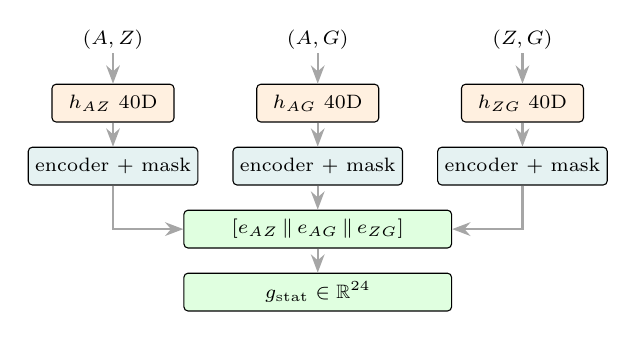
\begin{tikzpicture}[
  font=\scriptsize,
  >=Stealth,
  every node/.style={align=center},
  pair/.style={inner sep=1pt},
  box/.style={draw, rounded corners=1.5pt, inner sep=2.5pt, minimum height=0.48cm},
  h/.style={box, fill=orange!12, minimum width=1.55cm},
  enc/.style={box, fill=teal!10, minimum width=1.85cm},
  gout/.style={box, fill=green!12, minimum width=3.4cm},
  arr/.style={->, thick, draw=gray!70}
]
% top: ordered pairs
\node[pair] (paz) at (0.0,2.35) {$(A,Z)$};
\node[pair] (pag) at (2.6,2.35) {$(A,G)$};
\node[pair] (pzg) at (5.2,2.35) {$(Z,G)$};

% 40D vectors
\node[h] (haz) at (0.0,1.55) {$h_{AZ}$ 40D};
\node[h] (hag) at (2.6,1.55) {$h_{AG}$ 40D};
\node[h] (hzg) at (5.2,1.55) {$h_{ZG}$ 40D};

% encoder + mask
\node[enc] (eaz) at (0.0,0.75) {encoder + mask};
\node[enc] (eag) at (2.6,0.75) {encoder + mask};
\node[enc] (ezg) at (5.2,0.75) {encoder + mask};

% concat + g_stat
\node[gout] (cat) at (2.6,-0.05) {$[e_{AZ}\,\Vert\,e_{AG}\,\Vert\,e_{ZG}]$};
\node[gout] (gst) at (2.6,-0.85) {$g_{\mathrm{stat}}\in\mathbb{R}^{24}$};

\draw[arr] (paz) -- (haz);
\draw[arr] (pag) -- (hag);
\draw[arr] (pzg) -- (hzg);
\draw[arr] (haz) -- (eaz);
\draw[arr] (hag) -- (eag);
\draw[arr] (hzg) -- (ezg);
\draw[arr] (eaz.south) |- (cat.west);
\draw[arr] (eag) -- (cat);
\draw[arr] (ezg.south) |- (cat.east);
\draw[arr] (cat) -- (gst);
\end{tikzpicture}
}
\caption{Role-aware motif for $A\to G$: three ordered pair roles, each with a separate encoder and role mask, concatenated to $g_{\mathrm{stat}}\in\mathbb{R}^{24}$.}
\label{fig:taskA-motif}
\end{figure}

Fusion concatenates the branches,
\begin{equation}
g_{\mathrm{fusion}}=\bigl[g_{\mathrm{graph}}\parallel g_{\mathrm{stat}}\bigr]\in\mathbb{R}^{88},
\end{equation}
and maps $88\to 64\to 1$ (GELU, LayerNorm, dropout) to a single edge logit.

\section{Training and Evaluation}
\label{sec:taskA-train-eval}

\subsection{Training Objective}
\label{sec:taskA-loss}

For each candidate $i$ with logit $s_i$ and label $y_i\in\{0,1\}$,
\begin{equation}
\label{eq:taskA-sigmoid}
\hat{p}_{i}=\sigma(s_{i}),
\end{equation}
and parameters are optimized by weighted binary cross-entropy,
\begin{equation}
\label{eq:taskA-bce}
\mathcal{L}
=
-\frac{1}{N}
\sum_{i=1}^{N}
\bigl[
w_{+}\, y_{i}\log\hat{p}_{i}
+(1-y_{i})\log(1-\hat{p}_{i})
\bigr],
\end{equation}
with $w_{+}=N_{\mathrm{neg}}/N_{\mathrm{pos}}\approx 3$ under the $3{:}1$ negative-sampling ratio.
Weighting balances class contributions to the loss; it does not change the candidate inventory.

\subsection{Evaluation Metrics}
\label{sec:taskA-ap}

Model selection uses validation Average Precision (AP)~\cite{sklearn,davis2006},
\begin{equation}
\label{eq:taskA-ap}
\mathrm{AP}
=
\sum_{k}
\bigl(R_{k}-R_{k-1}\bigr)\,P_{k},
\end{equation}
where $P_k$ and $R_k$ are precision and recall at successive thresholds on the ranked score list ($R_0=0$).
This is the Average Precision summary of the ranked prediction list used throughout the thesis.
AP is appropriate for imbalanced link prediction because it emphasizes precision as recall increases.
The sealed test set is never used to choose architecture, representation or hyperparameters.
When discrete metrics such as $F_1$ are reported, the classification threshold is selected on validation only.

\subsection{Model and Training Configuration}
\label{sec:taskA-train-config}

Table~\ref{tab:taskA-train} lists the model and training configuration of the full model.
Six observational scenarios are evaluated; the official macro averages five scenarios and excludes the hidden-confounder scenario, which is reported for completeness only.

\begin{table}[!ht]
\centering
\footnotesize
\setlength{\tabcolsep}{4pt}
\caption{Task~A: model and training configuration.}
\label{tab:taskA-train}
\begin{tabular}{ll}
\toprule
Setting & Value \\
\midrule
Optimizer & Adam~\cite{kingma2015adam} \\
Learning rate & $10^{-3}$ \\
Weight decay & $5\times 10^{-4}$ \\
Max epochs & $200$ \\
Early stopping & patience $40$ on validation AP \\
Gradient clip & $1.0$ (global norm) \\
Normalization & LayerNorm in HGT and decoder blocks~\cite{ba2016layernorm} \\
HGT & $d=32$, $L=2$, $H=4$, dropout $0.25$~\cite{hu2020hgt} \\
Statistical branch & HCR-inspired $40$D pair vectors; MLP role encoders \\
Fusion & $64+24=88$ dimensional late fusion \\
Training seeds & five fixed seeds \\
Selection metric & validation AP \\
Official macro & mean over five scenarios (excludes hidden confounder) \\
\bottomrule
\end{tabular}
\end{table}

\section{Experimental Results}
\label{sec:taskA-results}

Results address three questions: which graph backbone to use, how much explicit statistical context contributes, and how the full model performs across observational scenarios.
Architecture and hyperparameters were selected on validation AP before sealed-test reporting.

\subsection{Architecture Comparison}
\label{sec:taskA-stage-a}

With the statistical branch disabled and a common decoder, HGT~\cite{hu2020hgt}, R-GCN~\cite{schlichtkrull2018rgcn}, GraphSAGE~\cite{hamilton2017graphsage} and GATv2~\cite{brody2022gatv2} were compared on the clean scenario.
Mean validation AP was approximately $0.729$ (HGT), $0.697$ (R-GCN), $0.671$ (GraphSAGE) and $0.650$ (GATv2).
HGT was retained as the structural encoder for all subsequent experiments.

\subsection{Contribution of Statistical Evidence}
\label{sec:taskA-stage-c}

With HGT fixed, explicit pairwise statistics were enriched progressively on the clean scenario (three seeds).
Validation AP rose from approximately $0.719$ with no pairwise statistics, to $0.840$ with signed Pearson $\phi$, $0.853$ with normalized mutual information, $0.913$ with an enriched multi-component representation, and $0.917$ with the full $40$-dimensional HCR-inspired vector.
The graph-only value $\approx 0.719$ in this ablation is not identical to the $\approx 0.729$ reported in the backbone comparison above: the former is the HGT-only arm of the statistical-enrichment ladder under a shared decoder and seed set, whereas the latter compares alternative graph encoders under a matched backbone-selection protocol.
Across the five official scenarios the full representation reached a macro validation AP of approximately $0.915$.
Removing the four derived dependence-summary dimensions reduced validation AP by about $0.008$ on average; the full vector was retained.

\subsection{Final Evaluation}
\label{sec:taskA-final}

Figure~\ref{fig:taskA-final-metrics} reports the full model under the official multi-scenario protocol.
Official macro test AP is $0.894$ and test AUROC is $0.967$.
Performance remains stable under selection bias, noisy documentation and related observational artefacts; the largest train--test AP gap appears in the multi-hospital scenario.

\begin{figure}[htbp]
\centering
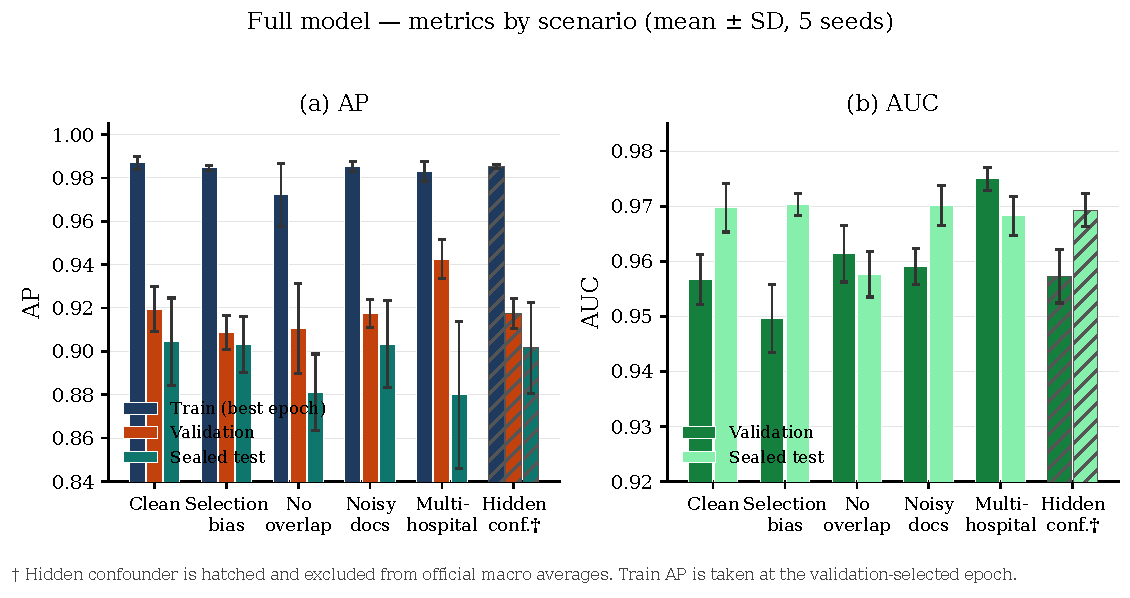
\includegraphics[width=\textwidth]{fig_final_metrics_per_scenario.pdf}
\caption{Task~A: final performance across observational scenarios.
Panel~(a): AP on the training partition (at the validation-selected epoch), on validation, and on the sealed test set.
Panel~(b): AUROC on validation and sealed test.
Bars are means over five training seeds; whiskers are one standard deviation.
The hatched scenario is excluded from official macro averages.
Official macro test AP is $0.894$ and test AUROC is $0.967$ (five-scenario mean; hidden confounder excluded).}
\label{fig:taskA-final-metrics}
\end{figure}


\chapter{Cross-Domain Validation of Task A. Last-FM*}
\label{ch:lastfm-proxy}
\label{ch:lastfm-ewaluacja}
\label{ch:lastfm-benchmark}

Last-FM* serves as a cross-domain validation of the Task~A modelling pattern: a heterogeneous graph encoder combined with explicit candidate-specific empirical context.
The transferred template is structural representation plus candidate-conditioned statistics fused in a decoder; the domain and prediction object change from pharmacotherapy edge classification to user--item ranking.

\section{Problem Formulation}
\label{sec:lastfm-problem}

We consider an implicit-feedback user--item ranking problem on a heterogeneous collaborative knowledge graph built from Last-FM listening events and Freebase-style music relations.
For a user $u$ and a candidate catalog item $X$, the model assigns a ranking score
\begin{equation}
\label{eq:lastfm-score}
s(u,X)=f_{\theta}(u,X;G_{\mathrm{train}},D_{\mathrm{train}}),
\end{equation}
where $G_{\mathrm{train}}$ is the collaborative knowledge graph available to the model and $D_{\mathrm{train}}$ denotes the training interaction data.
Higher scores indicate items ranked as more compatible with the user's observed training context.

The methodological question is whether ranking improves when an HGT representation of collaborative graph structure is combined with explicit candidate-specific empirical context derived from user interactions.

\section{Dataset and Collaborative Knowledge Graph}
\label{sec:lastfm-data}

\subsection{Leakage-corrected Last-FM*}
\label{sec:lastfm-data-star}

Experiments use Last-FM*, the leakage-corrected variant of the Last-FM benchmark associated with KGAT~\cite{wang2019kgat,shehzad2025lastfm}.
Overlapping train--test interactions are removed and interactions are re-split, yielding zero train--test interaction overlap.
Table~\ref{tab:lastfm-star-scale} compares the original dump with the corrected resource; Table~\ref{tab:lastfm-splits} states the working splits.

\begin{table}[htbp]
\centering
\caption{Last-FM dump versus leakage-corrected Last-FM*.}
\label{tab:lastfm-star-scale}
\begin{tabular}{lrr}
\toprule
Quantity & Original Last-FM dump & Last-FM* \\
\midrule
Users & 23{,}566 & 23{,}529 \\
Items & 48{,}123 & 48{,}123 \\
Official train interactions & 1{,}289{,}003 & 1{,}235{,}905 \\
Official test interactions & 423{,}635 & 306{,}914 \\
Users with train/test overlap & 17{,}290 & 0 \\
\bottomrule
\end{tabular}
\end{table}

\begin{table}[htbp]
\centering
\caption{Working splits used in the Last-FM* experiment. Official test remains sealed.}
\label{tab:lastfm-splits}
\begin{tabular}{lrl}
\toprule
Split & Interactions & Use \\
\midrule
model train & 1{,}111{,}803 & CKG construction, histories, statistical fitting, training \\
validation & 124{,}102 & checkpoint selection and full-catalog validation \\
test & 306{,}914 & sealed \\
\bottomrule
\end{tabular}
\end{table}

Validation is carved exclusively from the corrected training set under a fixed seed and a minimum-history constraint.
Full-catalog validation uses 23{,}163 users with at least one validation positive.
Working matrices contain binary implicit feedback only.

\subsection{Collaborative knowledge graph}
\label{sec:lastfm-ckg}

The HGT encoder operates on a heterogeneous collaborative knowledge graph with two node classes: user and entity.
Catalog items form a subset of the entity nodes; remaining entities come from the external music knowledge graph.

Message-passing relations comprise user--item interaction edges from the model-train split (and auxiliary reverse relations), together with entity--entity knowledge-graph relations under a deterministic cap of 250{,}000 edges (and their reverses).
Validation and test user--item interactions are absent from the message-passing graph.

\begin{figure}[htbp]
\centering
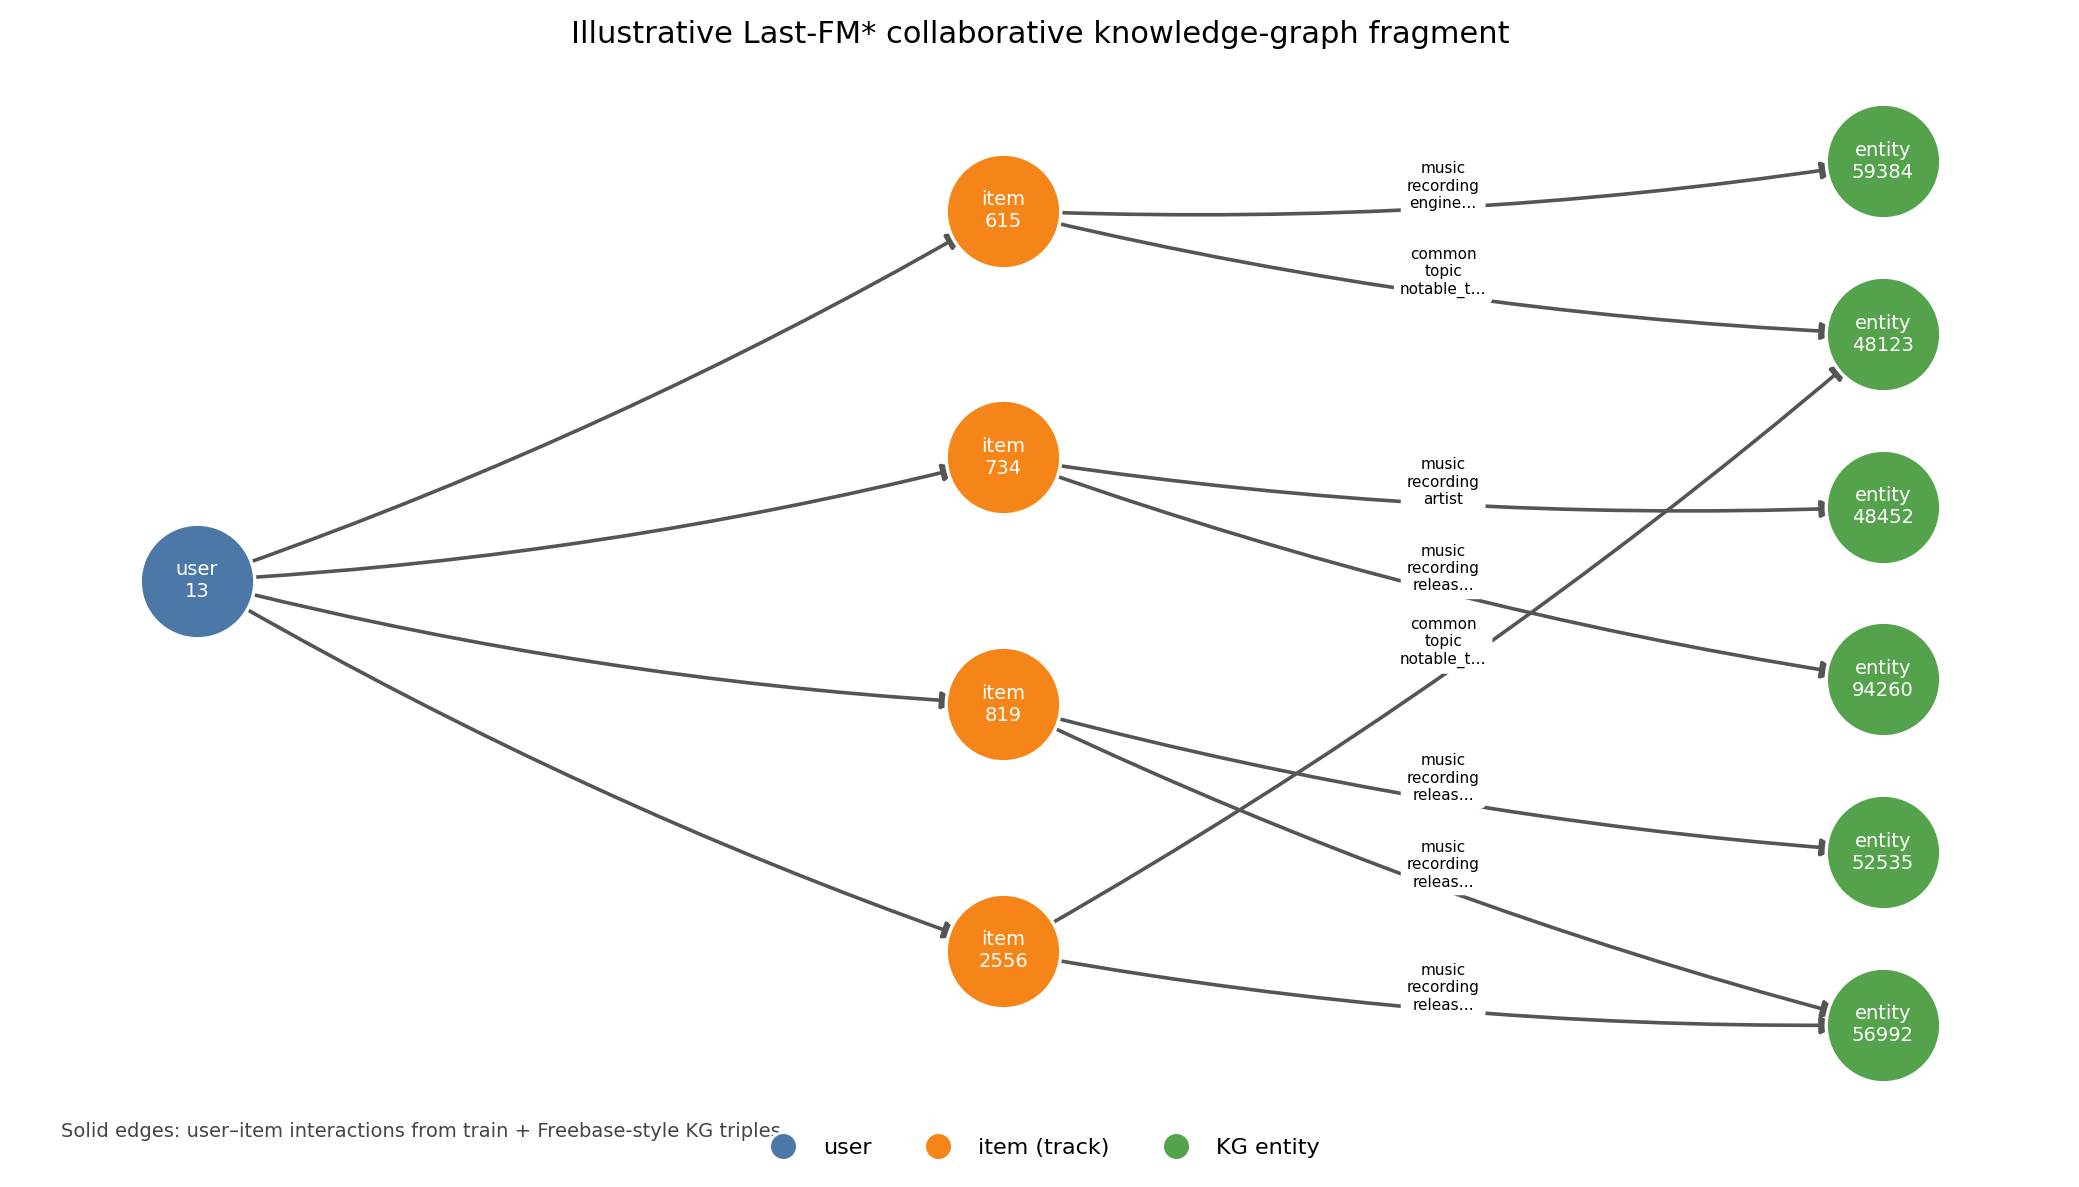
\includegraphics[width=\textwidth]{fig_lastfm_kg_fragment_networkx.png}
\caption{Illustrative fragment of the Last-FM* collaborative knowledge graph:
a user, training interactions, and Freebase-style entity neighbours of catalog items.}
\label{fig:lastfm-kg-fragment}
\end{figure}

\subsection{Training candidate pairs}
\label{sec:lastfm-negatives}

Positive training pairs are the observed model-train user--item interactions.
For each positive pair, four negative user--item pairs are sampled ($r_{\mathrm{neg}}=4$), excluding the user's known interaction history and known positive items.
The same candidate table is reused across representation ablations so that experiments change features rather than training examples.

\section{Model Architecture}
\label{sec:lastfm-arch}

\subsection{Architecture Overview}
\label{sec:lastfm-arch-overview}

Figure~\ref{fig:lastfm-arch-overview} summarizes the complete model.
An HGT encodes the collaborative knowledge graph; A5 and H3 supply candidate-specific empirical context; late fusion produces a main score; a zero-initialized LEG$_{K2}$ residual adds a second-order correction.

\begin{figure}[htbp]
\centering
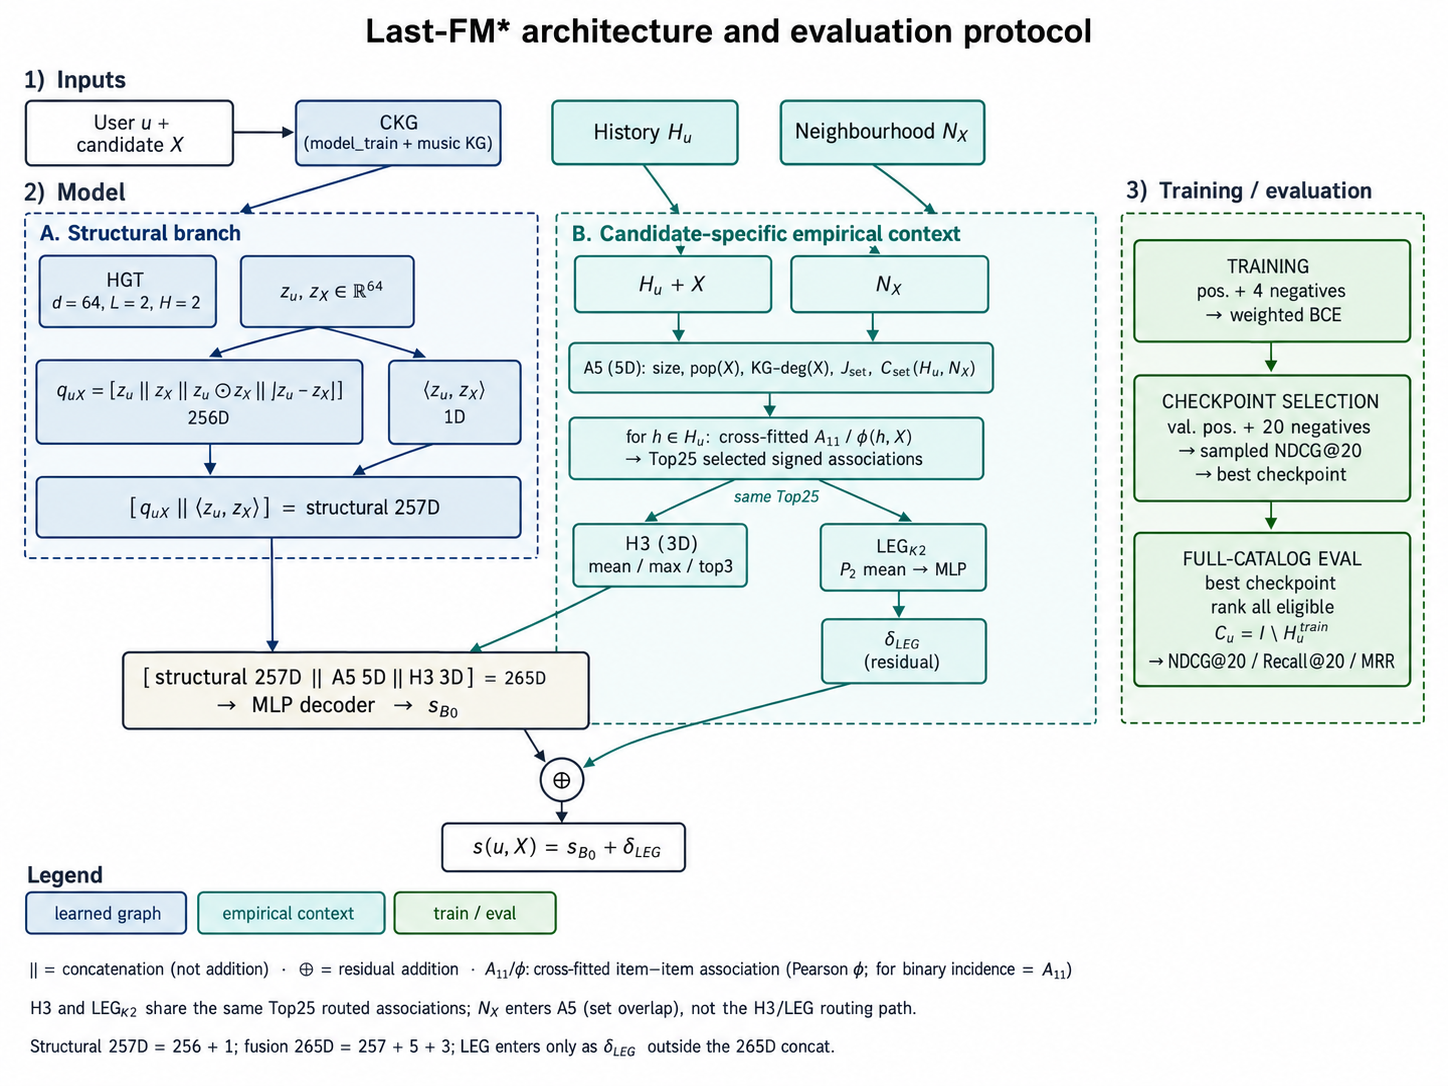
\includegraphics[width=\textwidth]{fig_lastfm_arch_simplified.png}
\caption{Last-FM* architecture.
Structural HGT yields $[q_{uX}\parallel\langle z_u,z_X\rangle]\in\mathbb{R}^{257}$.
A5 uses $H_u$, $X$ and $N_X$; routed Top25 associations feed both H3 and LEG$_{K2}$, with LEG entering only as residual $\delta_{\mathrm{LEG}}$.
Late fusion is $265$-dimensional ($\parallel$~=~concatenation; $\oplus$~=~residual addition).
The right column summarizes training and the two development evaluation levels; the sealed external benchmark is defined in Section~\ref{sec:lastfm-train-eval}.}
\label{fig:lastfm-arch-overview}
\end{figure}

\subsection{Structural Branch}
\label{sec:lastfm-hgt}

Each user and each entity receives a learnable embedding of dimension $d=64$, initialized with Xavier uniform weights and updated jointly with the decoder.
HGT node inputs are therefore learned embeddings; popularity and co-occurrence statistics are not injected into these tables.

The encoder uses
\begin{equation}
\label{eq:lastfm-hgt-hparams}
d=64,\qquad L=2,\qquad H=2,
\end{equation}
with dropout $0.1$.
After message passing on the training collaborative graph, let $z_u,z_X\in\mathbb{R}^{64}$ denote the embeddings of user $u$ and candidate item $X$.
The ordered pair representation is
\begin{equation}
\label{eq:lastfm-qux}
q_{uX}
=
\bigl[z_u \parallel z_X \parallel z_u\odot z_X \parallel |z_u-z_X|\bigr]
\in\mathbb{R}^{256},
\end{equation}
together with the scalar interaction $d_{uX}=\langle z_u,z_X\rangle$, for $257$ structural dimensions in total.

\subsection{Statistical Evidence Branch / Candidate-Specific Context}
\label{sec:lastfm-stats}

Candidate context is defined relative to the user's training history $H_u$ at several resolutions:
A5 compares the complete history with the candidate co-occurrence neighbourhood;
Pearson $\phi$ (A11) scores individual history items against $X$ for routing;
H3 summarizes the signed associations of the selected items;
LEG$_{K2}$ summarizes their second-order magnitude.

\begin{figure}[!ht]
\centering
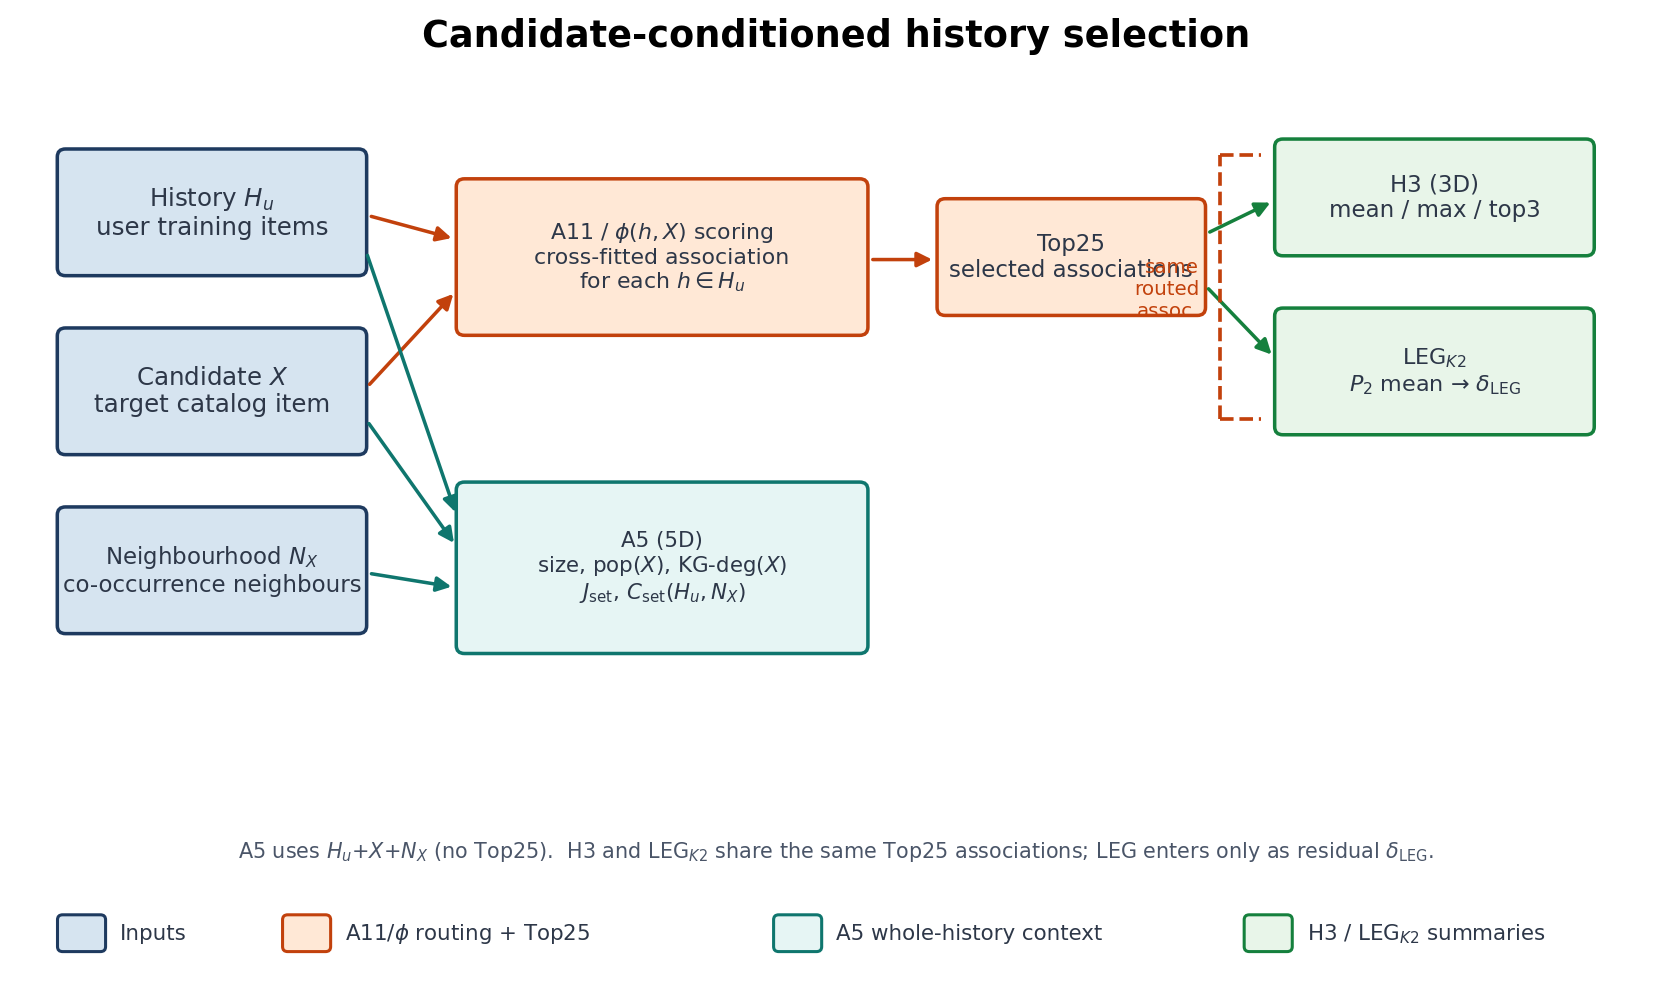
\includegraphics[width=0.92\textwidth]{fig_lastfm_context.png}
\caption{Candidate-conditioned history selection: A5 summarises whole-history context with $N_X$; Top25 routing by cross-fitted $A_{11}/\phi$ feeds both H3 and LEG$_{K2}$ from the same selected associations.}
\label{fig:lastfm-context}
\end{figure}

\paragraph{Cross-fitted item--item association.}
For history item $h$ and candidate $X$, co-occurrence across users yields contingency counts from which
\begin{equation}
\label{eq:lastfm-phi}
\phi(h,X)
=
\frac{N n_{11}-n_h n_X}
{\sqrt{n_h(N-n_h)\,n_X(N-n_X)}},
\qquad
\phi\in[-1,1].
\end{equation}
Association counts for user $u$ are computed from a five-fold partition of training interactions, excluding the fold that contains $u$.
Validation and test interactions never enter these counts.
The candidate co-occurrence neighbourhood is $N_X=\{j\neq X:n_{11}(j,X)>0\}$.

\paragraph{A5: full-history candidate context.}
\begin{equation}
\label{eq:lastfm-A5}
\begin{aligned}
A(u,X)
=
\bigl[
&\log(1+|H_u|),\;
\log(1+\mathrm{pop}(X)),\;
\log(1+\deg_{\mathrm{KG}}(X)),\\
&\qquad
J_{\mathrm{set}}(H_u,N_X),\;
C_{\mathrm{set}}(H_u,N_X)
\bigr]
\in\mathbb{R}^{5},
\end{aligned}
\end{equation}
where
\begin{equation}
\label{eq:lastfm-Jset}
J_{\mathrm{set}}(H_u,N_X)=\frac{|H_u\cap N_X|}{|H_u\cup N_X|},
\qquad
C_{\mathrm{set}}(H_u,N_X)=\frac{|H_u\cap N_X|}{\sqrt{|H_u|\,|N_X|}},
\end{equation}
with empty-set cases mapped to zero.
A5 is standardized on training pairs only.

\paragraph{Candidate-conditioned routing and H3.}
For each $h\in H_u\setminus\{X\}$, the routing score is $v(h,X)=\phi(h,X)$.
Alternative association criteria (Jaccard, cosine, co-occurrence, MI, NPMI, $G^{2}$) were screened under a fixed Top25 budget; signed Pearson $\phi$ was retained.
The Top$K$ items with $K=\min\bigl(25,|H_u\setminus\{X\}|\bigr)$ are summarized by
\begin{equation}
\label{eq:lastfm-H3}
H_3(u,X)=\bigl[\mathrm{mean}(v),\;\mathrm{max}(v),\;\mathrm{top3mean}(v)\bigr]\in\mathbb{R}^{3},
\end{equation}
using signed values; an empty routed history is $[0,0,0]$.
H3 is standardized on training pairs only.

\paragraph{LEG$_{K2}$ residual.}
The same Top-$K$ association coefficients selected for H3 are additionally summarized using the second Legendre polynomial,
\begin{equation}
\label{eq:lastfm-L2}
L_2(u,X)=\frac{1}{K}\sum_{k=1}^{K}P_2(v_k),
\qquad
P_2(v)=\frac{3v^{2}-1}{2}.
\end{equation}
While H3 preserves signed first-order summaries of the selected associations, $L_2$ provides a complementary nonlinear summary of their magnitude.
Because $P_2$ is an even function, strong positive and negative associations both contribute through their squared magnitude, allowing the residual branch to capture structure that is not represented by the signed mean or maximum alone.

Higher-order Legendre terms were also considered during model development.
The third-order term $P_3$ retains sign and therefore overlaps more strongly with information already represented by the signed H3 statistics, whereas the fourth-order term $P_4$ places greater emphasis on extreme coefficients and can be more sensitive to variation in the relatively small routed set ($K\le 25$).
The second-order term was therefore retained as the most compact complementary summary of the routed association context:
\begin{equation*}
\mathrm{Top}25
\;\longrightarrow\;
\begin{cases}
\mathrm{H3}: & \text{signed summary},\\
L_2: & \text{nonlinear magnitude summary}.
\end{cases}
\end{equation*}

The scalar $L_2(u,X)$ is standardized using training pairs and passed through a small residual MLP producing $\delta_{\mathrm{LEG}}(u,X)$.
The final linear layer of this branch is initialized to zero, so the residual contribution is initially neutral and is learned only when supported by the training signal.

\subsection{Fusion and Prediction}
\label{sec:lastfm-fusion}

The main late-fusion input is
\begin{equation}
\label{eq:lastfm-265}
g_{uX}
=
\bigl[q_{uX}\parallel d_{uX}\parallel A(u,X)\parallel H_3(u,X)\bigr]
\in\mathbb{R}^{265}.
\end{equation}
A decoder $265\to 128\to 64\to 1$ (LayerNorm, GELU, dropout) produces $s_{B0}(u,X)$.
LEG$_{K2}$ is not concatenated into $g_{uX}$; it enters only as an additive residual.
The final ranking score is
\begin{equation}
\label{eq:lastfm-score-final}
s(u,X)=s_{B0}(u,X)+\delta_{\mathrm{LEG}}(u,X).
\end{equation}

\section{Training and Evaluation}
\label{sec:lastfm-train-eval}

The Last-FM* experiments use three evaluation levels corresponding to different stages of model development.
Sampled validation is used for checkpoint selection, full-catalog validation for architectural ablation, and the sealed external benchmark for the final comparison with classical recommenders.
Although NDCG@20 is used in more than one stage, the corresponding values are interpreted within their respective candidate universes and experimental roles.

\subsection{Training Objective}
\label{sec:lastfm-train}

For each training pair with ranking score $s_i$ and label $y_i\in\{0,1\}$,
\begin{equation}
\hat{p}_i=\sigma(s_i),
\end{equation}
is used only inside weighted binary cross-entropy ($w_{+}\approx 4$ under the $4{:}1$ candidate construction).
The quantity $s(u,X)$ itself is a ranking score, not a calibrated interaction probability.
Optimization uses Adam (learning rate $10^{-3}$, weight decay $10^{-4}$), ReduceLROnPlateau on sampled validation NDCG@20, batch size $4096$, and early stopping with patience $8$ on the same sampled metric.
Figure~\ref{fig:lastfm-training-protocol} shows a representative development learning curve for seed~$303$, with the selected checkpoint marked.
Architecture and per-seed epochs were frozen under this sampled rule before any sealed-test evaluation; full-catalog development metrics and the sealed external benchmark are computed only after freeze and are never used to re-select the epoch.

\begin{figure}[htbp]
\centering
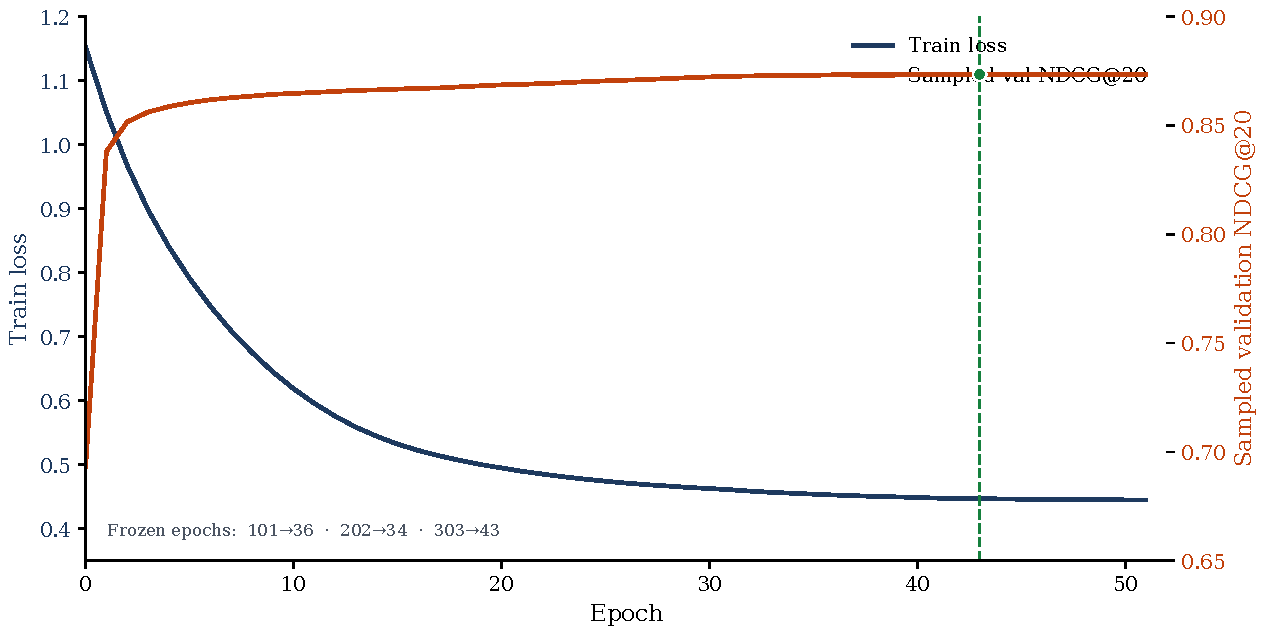
\includegraphics[width=\textwidth]{fig_lastfm_training_protocol.pdf}
\caption{Development training dynamics for seed~$303$ of the full Last-FM* model: training loss and sampled validation NDCG@20 versus epoch.
The dashed line marks the selected checkpoint (epoch~$43$).
Seeds~$101$ and~$202$ were frozen under the same sampled rule at epochs~$36$ and~$34$.}
\label{fig:lastfm-training-protocol}
\end{figure}

\subsection{Checkpoint selection with sampled NDCG@20}
\label{sec:lastfm-sampled-val}

Sampled validation NDCG@20 was used for checkpoint selection and early stopping during model development.
For each validation positive, the candidate set consisted of the relevant item and $20$ sampled negatives not present in the user's observed history.
To limit the contribution of highly active users, at most $10$ validation positives per user were included.

This sampled protocol provides a computationally efficient ranking signal during training.
It is used exclusively for model selection and is not interpreted as catalog-scale recommendation performance.

\subsection{Development full-catalog evaluation}
\label{sec:lastfm-fullcatalog}

After checkpoint selection, architectural variants were evaluated against the full eligible catalog.
For user $u$, the candidate set was defined as
\begin{equation}
\label{eq:lastfm-Cu}
\mathcal{C}_u=I\setminus H_u^{(\mathrm{model\_train})},
\end{equation}
where $I$ denotes the item catalog and $H_u^{(\mathrm{model\_train})}$ contains items already observed for that user in the model-training data.

Performance was reported using NDCG@20, Recall@20, and MRR.
This evaluation was used to quantify the contribution of the candidate-specific empirical components---A5, H3, and the LEG$_{K2}$ residual---relative to the structural HGT baseline under catalog-scale ranking.

\subsection{Sealed external benchmark}
\label{sec:lastfm-sealed}

The final external benchmark was conducted only after the model specification and per-seed training schedule had been fixed on development data.
The final models were refitted on the complete corrected training population,
\begin{equation}
\label{eq:lastfm-Dtrain-ext}
\mathcal{D}_{\mathrm{train}}^{\mathrm{external}}
=
\mathcal{D}_{\mathrm{model\_train}}
\cup
\mathcal{D}_{\mathrm{validation}},
\end{equation}
and evaluated on the previously unseen corrected Last-FM* test split using the pinned IntentAwareRS holdout evaluator.

The proposed model and the classical recommendation baselines were evaluated under the same full-catalog candidate-space rules and reported using NDCG@20, Recall@20, and MRR.
This stage therefore provides the matched external comparison used for the final benchmark results.

\subsection{Computational note}
\label{sec:lastfm-compute}

Full-catalog neural evaluation on Last-FM* was computationally demanding on the available local hardware because scores had to be produced for a catalog of $48{,}123$ items for each eligible user.
This constrained the breadth of additional convergence and hyperparameter studies.
The external comparison therefore follows the prespecified model specification rather than an extensive post-hoc search over training budgets.

\section{Experimental Results}
\label{sec:lastfm-results}

\subsection{Architecture Comparison}
\label{sec:lastfm-backbone}

HGT width, depth and number of attention heads were compared under a common development protocol with the decoder family held fixed.
The selected configuration is $d=64$, $L=2$, $H=2$ with dropout $0.1$; larger width, deeper stacks or additional heads did not justify replacement.
Table~\ref{tab:lastfm-train} summarizes the frozen training and model settings of the full Last-FM* specification used in all subsequent development and sealed evaluations.

\begin{table}[!ht]
\centering
\footnotesize
\setlength{\tabcolsep}{4pt}
\caption{Last-FM*: model and training configuration.}
\label{tab:lastfm-train}
\begin{tabularx}{\textwidth}{@{}>{\raggedright\arraybackslash}p{2.85cm} X@{}}
\toprule
Setting & Value \\
\midrule
Optimizer & Adam~\cite{kingma2015adam} \\
Learning rate & $10^{-3}$ \\
Weight decay & $10^{-4}$ \\
LR schedule & ReduceLROnPlateau on sampled validation NDCG@20;
  factor~$0.5$, patience~$3$, $\mathrm{min\_lr}=6.25\times 10^{-5}$ \\
Batch size & $4096$ \\
Max epochs & $120$ \\
Early stopping & patience~$8$ on sampled validation NDCG@20 \\
Loss & weighted binary cross-entropy ($w_{+}\approx 4$; $4{:}1$ candidate construction) \\
HGT & $d=64$, $L=2$, $H=2$, dropout~$0.1$~\cite{hu2020hgt} \\
Structural pair & $q_{uX}\in\mathbb{R}^{256}$ plus graph dot $\Rightarrow 257$D \\
Explicit context & A5 ($5$D), H3 ($3$D), LEG$_{K2}$ residual \\
Main decoder & $265\to 128\to 64\to 1$ (LayerNorm, GELU, dropout~$0.2$) \\
LEG$_{K2}$ branch & $1\to 16\to 1$ (GELU; final linear zero-initialized) \\
Training seeds & $\{101,202,303\}$ \\
Selection metric & sampled validation NDCG@20 \\
Frozen epochs & seed~$101\to 36$, seed~$202\to 34$, seed~$303\to 43$ \\
\bottomrule
\end{tabularx}
\end{table}

\subsection{Contribution of Statistical Evidence}
\label{sec:lastfm-ablation}

With the HGT backbone fixed, a controlled ablation ladder isolates explicit candidate context (Table~\ref{tab:lastfm-ablation}, Figure~\ref{fig:lastfm-ablation-bars}), using seeds $\{101,202,303\}$:
\begin{enumerate}
\item HGT only ($257$-dimensional structural input);
\item HGT + A5;
\item HGT + A5 + H3;
\item full model (A5 + H3 plus the LEG$_{K2}$ residual).
\end{enumerate}

\begin{table}[htbp]
\centering
\footnotesize
\caption{Last-FM*: development ablation results.
Sampled NDCG@20 is the checkpoint-selection metric; full-catalog NDCG@20 and Recall@20 evaluate the same checkpoints on the eligible validation catalog.
These are development validation results and are used to isolate the contribution of explicit candidate-specific context.
They are not the final external benchmark.}
\label{tab:lastfm-ablation}
\setlength{\tabcolsep}{2.6pt}
\begin{tabular}{@{}lcccc@{}}
\toprule
Variant & Main decoder & Sampled NDCG@20 & Full-cat.\ NDCG@20 & Full-cat.\ Recall@20 \\
\midrule
HGT only & 257D & \(0.4755\) & \(0.0093\) & \(0.0169\) \\
HGT + A5 & 262D & \(0.7908\) & \(0.0640\) & \(0.1128\) \\
HGT + A5 + H3 & 265D & \(0.8729\) & \(0.2321\) & \(0.3647\) \\
Full model (+ LEG$_{K2}$) & 265D + residual & \(0.8733\) & \(0.2764\) & \(0.3768\) \\
\bottomrule
\end{tabular}
\end{table}

\begin{figure}[htbp]
\centering
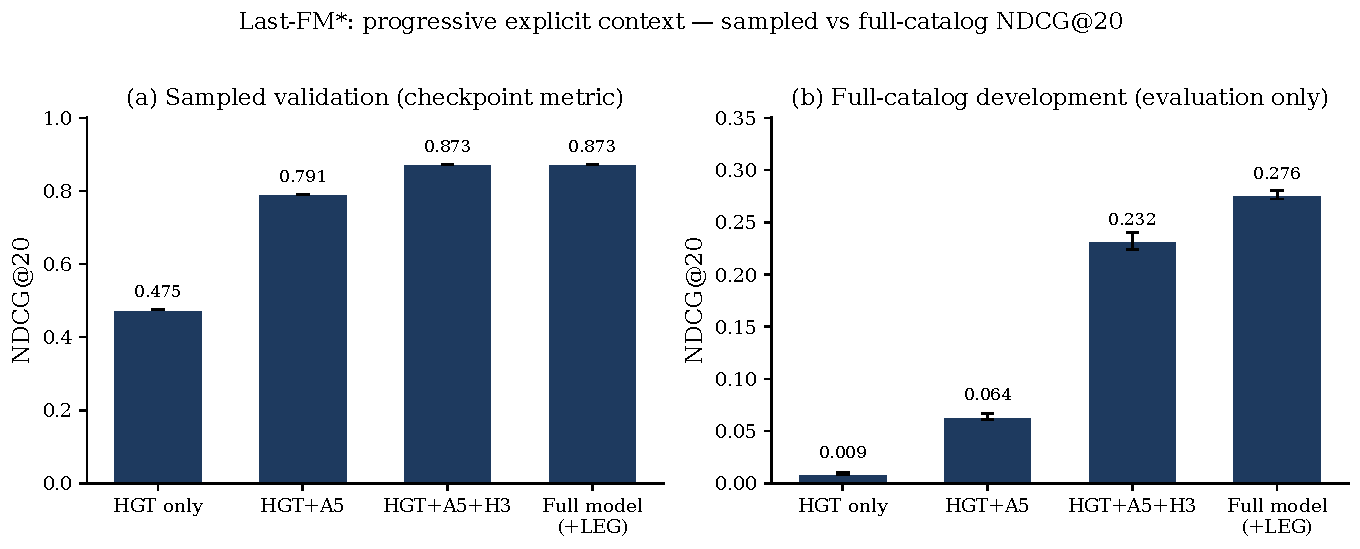
\includegraphics[width=\textwidth]{fig_lastfm_ablation_bars.pdf}
\caption{Last-FM* development ablation ladder.
Panel~(a): sampled validation NDCG@20 used for checkpoint selection.
Panel~(b): full-catalog development NDCG@20 of the same checkpoints.
Error bars show the seed standard deviation over three training seeds.
The panels use different $y$-axis scales because they evaluate different candidate universes under the same NDCG@20 formula.
This figure is not an external baseline comparison.}
\label{fig:lastfm-ablation-bars}
\end{figure}

The controlled ablation demonstrates that explicit candidate-specific empirical context substantially improves the neural graph model relative to its HGT-only counterpart.
A5 introduces the first large improvement on both development protocols.
H3 produces the largest full-catalog increase.
LEG$_{K2}$ changes sampled NDCG@20 by only about $0.0004$ relative to HGT+A5+H3, while adding a further full-catalog gain of about $0.044$ NDCG@20.
The development ablation addresses the contribution of the proposed representation within the neural model family.
It does not by itself establish superiority over strong collaborative-filtering baselines.

\subsection{Full-catalog development ranking and classical baseline}
\label{sec:lastfm-fullrank}

Epochs were selected using sampled validation NDCG@20; full-catalog development metrics were then computed without re-selection (Table~\ref{tab:lastfm-dev-seeds}).

\begin{table}[htbp]
\centering
\footnotesize
\caption{Full-model full-catalog development metrics by seed (model train $\to$ validation).
Sampled NDCG@20 selected the epoch; full-catalog metrics are evaluation only.}
\label{tab:lastfm-dev-seeds}
\label{tab:lastfm-true-final}
\setlength{\tabcolsep}{3pt}
\begin{tabular}{@{}crrrrr@{}}
\toprule
Seed & Best epoch & Sampled NDCG@20 & Full-cat.\ NDCG@20 & Recall@20 & MRR \\
\midrule
101 & 36 & 0.873224 & 0.277432 & 0.375599 & 0.356988 \\
202 & 34 & 0.873253 & 0.279879 & 0.378722 & 0.359681 \\
303 & 43 & 0.873515 & 0.271886 & 0.376197 & 0.343391 \\
\midrule
Mean \(\pm\) SD & --- & \(0.8733\pm 0.0002\) & \(0.2764\pm 0.0041\) & \(0.3768\) & \(0.3534\) \\
\bottomrule
\end{tabular}
\end{table}

\begin{table}[htbp]
\centering
\small
\caption{Full-catalog development NDCG@20 by seed for the ablation layers without LEG$_{K2}$.}
\label{tab:lastfm-fullrank-ablation}
\setlength{\tabcolsep}{4pt}
\begin{tabular}{crrr}
\toprule
Seed & HGT only & HGT+A5 & HGT+A5+H3 \\
\midrule
101 & 0.008548 & 0.064571 & 0.227969 \\
202 & 0.009520 & 0.060866 & 0.241332 \\
303 & 0.009935 & 0.066630 & 0.227054 \\
\midrule
Mean & \(0.0093\) & \(0.0640\) & \(0.2321\) \\
\bottomrule
\end{tabular}
\end{table}

For the full model, mean full-catalog development NDCG values were additionally $\mathrm{NDCG}@5=0.2336$ and $\mathrm{NDCG}@10=0.2503$; HitRate@20 was approximately $0.664$.

Under the same full-catalog development protocol, a matched RP$3\beta$ reference already reached NDCG@20 $=0.3227$, Recall@20 $=0.4122$ and MRR $=0.4183$, exceeding the proposed full model (NDCG@20 $=0.2764$).
Importantly, RP$3\beta$ already outperformed the proposed model under full-catalog development evaluation.
The sealed external benchmark therefore evaluates whether this qualitative ordering persists on the previously unseen corrected test split.

\subsection{Sealed external benchmark}
\label{sec:lastfm-sealed-results}

Table~\ref{tab:lastfm-sealed-baselines} reports classical baselines on the sealed corrected test under the pinned holdout evaluator after fitting on $\mathrm{TRAIN\_EXTERNAL}$.
RP$3\beta$ is the strongest classical baseline (NDCG@20 $=0.2318$, Recall@20 $=0.2588$).

\begin{table}[htbp]
\centering
\small
\caption{Last-FM*: sealed external benchmark results for classical recommenders fitted on $\mathrm{TRAIN\_EXTERNAL}$ and evaluated once on the corrected Last-FM* test with the pinned holdout evaluator.
Primary comparison metrics are NDCG@20 and Recall@20.}
\label{tab:lastfm-sealed-baselines}
\begin{tabular}{@{}lcc@{}}
\toprule
Model & NDCG@20 & Recall@20 \\
\midrule
TopPop & 0.0091 & 0.0153 \\
UserKNN & 0.1622 & 0.1819 \\
ItemKNN & 0.2051 & 0.2369 \\
P3$\alpha$ & 0.2035 & 0.2385 \\
\textbf{RP$3\beta$} & \textbf{0.2318} & \textbf{0.2588} \\
\bottomrule
\end{tabular}
\end{table}

Table~\ref{tab:lastfm-sealed-proposed} reports the proposed model under the same sealed protocol.
All three prespecified seeds are complete; the mean $\pm$ SD is computed over seeds~$101$, $202$ and~$303$.

\begin{table}[htbp]
\centering
\small
\caption{Last-FM*: sealed external benchmark results for the proposed full model under the frozen epoch schedule.
Mean $\pm$ SD is over the three prespecified training seeds.}
\label{tab:lastfm-sealed-proposed}
\begin{tabular}{@{}crrr@{}}
\toprule
Seed & Frozen epoch & NDCG@20 & Recall@20 \\
\midrule
101 & 36 & 0.1685 & 0.2123 \\
202 & 34 & 0.1762 & 0.2167 \\
303 & 43 & 0.1706 & 0.2127 \\
\midrule
Mean \(\pm\) SD & --- & \(0.1718\pm 0.0040\) & \(0.2139\pm 0.0024\) \\
\bottomrule
\end{tabular}
\end{table}

Figure~\ref{fig:lastfm-sealed-benchmark} compares classical baselines and the proposed mean under the same sealed protocol.

\begin{figure}[htbp]
\centering
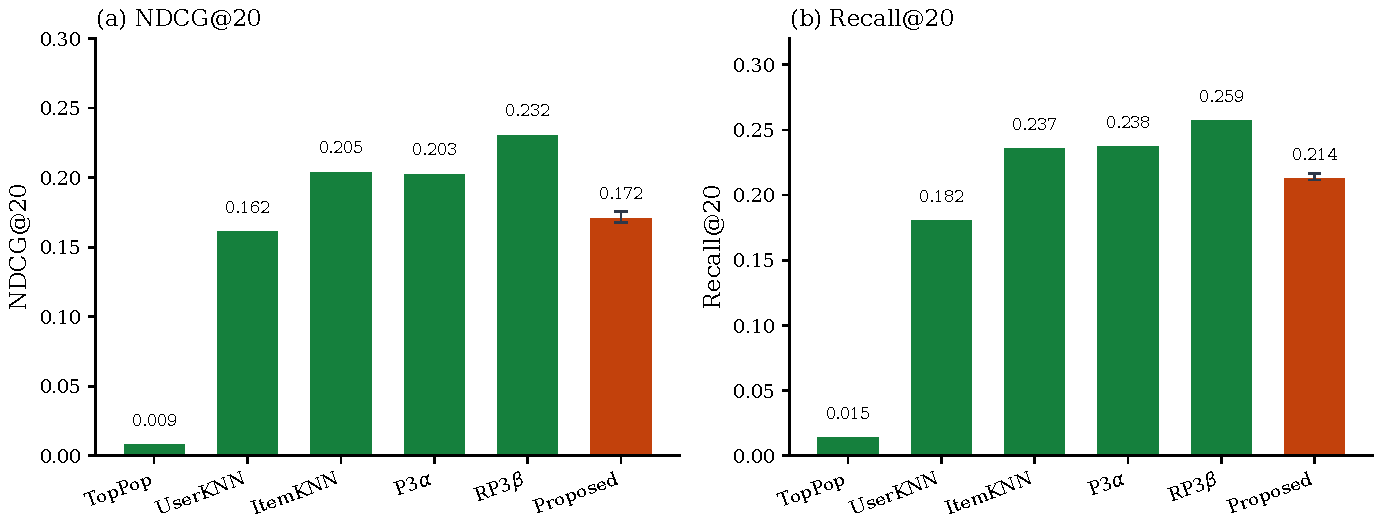
\includegraphics[width=\textwidth]{fig_lastfm_sealed_benchmark.pdf}
\caption{Sealed external Last-FM* benchmark.
NDCG@20 and Recall@20 for classical recommendation baselines and the proposed model under the same full-catalog holdout evaluation protocol.
The proposed-model bars report the mean across the three prespecified training seeds, with error bars indicating one standard deviation.}
\label{fig:lastfm-sealed-benchmark}
\end{figure}

On the sealed external test, RP$3\beta$ was the strongest classical baseline, reaching NDCG@20 $=0.2318$ and Recall@20 $=0.2588$.
The proposed model reached mean NDCG@20 $=0.1718\pm 0.0040$ and Recall@20 $=0.2139\pm 0.0024$ across seeds~$101$, $202$ and~$303$ (per-seed NDCG@20: $0.1685$, $0.1762$, $0.1706$).
Seed~$202$ is the strongest of the three, but all three seeds remain below RP$3\beta$, ItemKNN and P3$\alpha$ on NDCG@20, which is consistent with the development ordering in which RP$3\beta$ already exceeded the proposed model.
The external benchmark highlights an important distinction between improving a neural graph model and achieving benchmark dominance: explicit candidate-specific statistical context provides substantial ranking signal beyond HGT alone, but strong classical collaborative-filtering methods remain competitive and, in this benchmark, can outperform the more complex neural architecture.
Full-catalog development and sealed external numbers must not be subtracted as if they were the same experiment.

\chapter{Task B. Patient-Level Endpoint Prediction}
\label{ch:taskB-method}
\label{ch:taskB-eval}

\section{Problem Formulation}
\label{sec:taskB-problem}

Task B is formulated as multi-label node classification on a heterogeneous,
per-patient graph, in order to predict clinical outcomes.
Instead of building one global graph and treating patients as additional nodes,
every patient $p$ is represented as a copy of the same fixed SPG~v3, with node
feature vectors derived from that patient's covariates.

Formally, patient $p$ is represented by the attributed graph
$G_p = (V, E, x_p)$, where $x_p$ denotes the patient-specific node features.
The topology $(V, E)$ is shared across the cohort.
The node set $V$ comprises six semantic categories:
\begin{itemize}
    \item \textit{patient\_context} --- baseline characteristics such as age, sex, or alcohol use;
    \item \textit{drug\_exposure} --- medications taken, such as anticoagulants, diuretics, or opioids;
    \item \textit{mechanism} --- biological or pharmacodynamic processes such as slowed drug breakdown, sodium--water imbalance, or poor kidney blood flow;
    \item \textit{adr\_or\_intermediate\_state} --- visible medical states such as a rise in creatinine, ECG-measured QT prolongation, or bleeding;
    \item \textit{observation\_or\_selection} --- testing, documentation, and care-selection variables such as laboratory monitoring or recorded clinical checks;
    \item \textit{clinical\_endpoint} --- clinical outcomes being predicted, described in \cref{subsec:taskB-prediction-targets}.
\end{itemize}
These node types encode a causal pathway towards a clinical outcome:
signals propagate along the edges of SPG~v3 from context and drug exposure,
through mechanisms and visible medical states, to the endpoints.
In general, heart failure (\textit{patient\_context}) together with an NSAID
(\textit{drug\_exposure}) may reduce kidney blood flow (\textit{mechanism}),
become visible as a rise in creatinine
(\textit{adr\_or\_intermediate\_state}), and culminate in AKI
(\textit{clinical\_endpoint}); laboratory monitoring of creatinine is an
\textit{observation\_or\_selection} node on the same pathway.
Which of those nodes are actually on for a given patient is encoded in $x_p$.
\Cref{fig:patient_dag} shows one such realisation ending in AKI: filled nodes
are this patient's active context, drugs and mechanisms, whereas outlined nodes
(for example NSAID, heart failure, or a creatinine rise) remain inactive
mediators on the shared schema.
The aim of Task~B is to estimate endpoint
risk from the entire patient-specific graph as described above.

\begin{figure}[H]
    \centering
    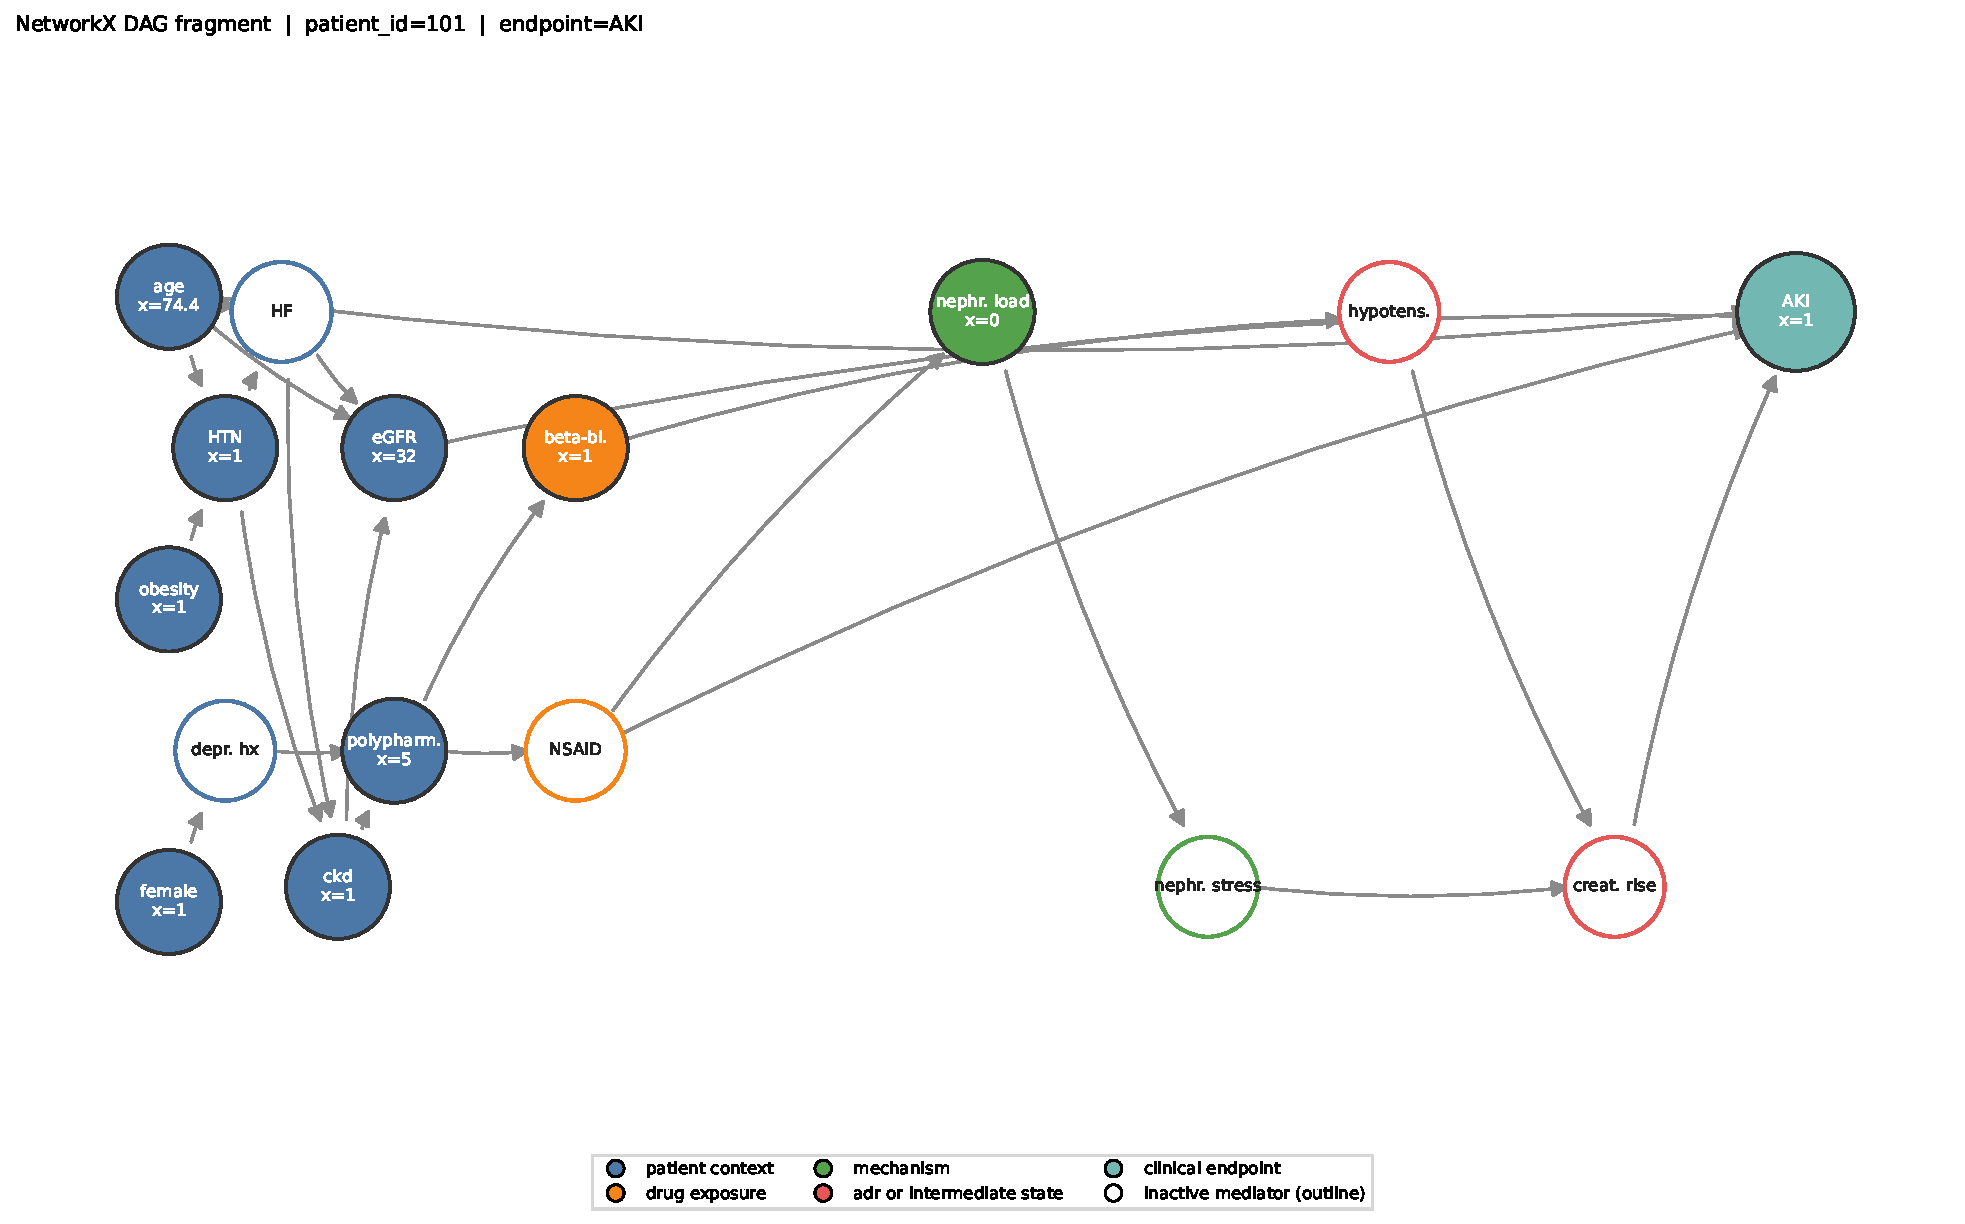
\includegraphics[width=\textwidth]{patient_dag_101.pdf}
    \caption{Exemplary per-patient causal DAG for one synthetic patient (id~101).
    The full SPG~v3 is shared across the cohort; this figure keeps only the
    AKI-relevant fragment so that the left-to-right causal layers remain readable.
    Filled nodes are active for this patient; outlined nodes are inactive mediators
    on the same paths.}
    \label{fig:patient_dag}
\end{figure}

Assuming that \(\mathcal{V}_{\text{target}} \subset V\) is the set of
endpoint nodes used as prediction targets,
for each patient $p$ and target node $v \in \mathcal{V}_{\text{target}}$
the binary label $y_{p,v}$ indicates whether the endpoint occurs.
A shared heterogeneous GNN $f_\theta$ produces a separate probability for each
endpoint from the same encoded graph; $v$ is a concrete clinical endpoint such
as QT arrhythmia, Falls, Serotonin syndrome, or AKI:
\begin{equation}
\begin{gathered}
\hat{y}_{p,v} = \sigma\big(f_\theta(G_p)_v\big),
\quad v \in \mathcal{V}_{\text{target}}, \\[0.4em]
{\scriptstyle
G_p=(V,E,x_p),\ 
f_\theta\text{ --- heterogeneous GNN shared across patients},\ 
v\text{ --- clinical endpoint node}
}
\end{gathered}
\end{equation} 

\section{Patient-Level Graph Representation}
\label{subsec:taskb_data}

The input graph for the node classification task is built from: 

\begin{enumerate}[label=\alph*)]
    \item \textbf{nodes}
    \item \textbf{edges}
    \item \textbf{per-scenario patient sample table} 
\end{enumerate}

These components are assembled into a heterogeneous per-patient graph representation
 whose elements are summarised in \cref{tab:heterodata_components}.

\begin{table}[H]
    \centering
    \caption{Components of the per-patient heterogeneous graph representation.}
    \label{tab:heterodata_components}
    \begin{tabularx}{\textwidth}{@{}l X@{}}
        \toprule
        \textbf{Component} & \textbf{Description} \\
        \midrule
        Node types &
        Six semantic categories of nodes shared across all patient graphs: \texttt{patient\_context}, \texttt{drug\_exposure}, \texttt{mechanism}, \texttt{adr\_or\_intermediate\_state}, \texttt{observation\_or\_selection}, and \texttt{clinical\_endpoint}. \\
        \addlinespace
        Relations &
        Keyed by \texttt{(src\_type, "to", dst\_type)};
        \texttt{edge\_type} is encoded as a one-hot block inside
        \texttt{edge\_attr}. This keeps the number of distinct convolutional
        relation modules in \texttt{HeteroConv} small while still letting
        edge-type information reach the message function. \\
        \addlinespace
        Edge attributes (\texttt{edge\_attr}) &
        Fixed-length vector per edge (see \cref{tab:edge_attr_layout}): signed
        effect \texttt{effect\_size}$\times$\texttt{effect\_sign}, audit scalars
        \texttt{activation\_frequency}, \texttt{mechanistic\_confidence},
        \texttt{evidence\_weight}, and a one-hot \texttt{edge\_type} block. \\
        \addlinespace
        Node features (\texttt{x}) &
        The patient's observed values for a node \\
        \bottomrule
    \end{tabularx}
\end{table}

Patient observations are encoded as node features.
The AKI fragment in \cref{fig:patient_dag} is the running example of
Section~\ref{sec:taskB-problem}: filled nodes follow this patient's $x_p$,
outlined nodes are inactive mediators on the same directed paths.

Two structural exclusion mechanisms are applied before any feature is computed: 
\begin{enumerate}[label=\alph*)]
    \item nodes flagged \texttt{exclude\_from\_observed\_model} or \texttt{is\_latent} (hidden confounders); 
    \item nodes that are structural descendants of any endpoint in the DAG (e.g. documentation nodes such as 
    \texttt{hospital\_contact}, \texttt{fall\_reported}, which are caused by the endpoint rather than causal parents of it)
\end{enumerate}

 All normalization statistics (mean/std for continuous node values) 
 and all statistical evidence features (\cref{subsec:hcr_application}) are computed exclusively on the training split of patients, to 
 prevent both node-level and patient-level information leakage across splits.

\subsection{Prediction targets}
\label{subsec:taskB-prediction-targets}
Although the knowledge graph defines 13 
clinical outcomes nodes, the model is trained and evaluated on a
subset of 11 clinical endpoints, excluding
%\texttt{AKI}, \texttt{DILI}, \texttt{Depression}, \texttt{Delirium},
%\texttt{GI\_bleeding}, \texttt{Hyponatremia}, \texttt{Hyperkalemia},
%\texttt{QT\_arrhythmia}, \texttt{Serotonin\_syndrome},
%\texttt{Rhabdomyolysis}, and \texttt{Lactic\_acidosis}.
%The remaining two endpoints---
\texttt{Hospitalization} and
\texttt{Falls}. They are retained in the per-patient graph topology and in
patient labels, but are excluded from the multi-target prediction head.

This choice follows both the graph structure and the clinical scope of
the task. \texttt{Hospitalization} was excluded because the DAG models it
as a downstream consequence of other endpoints
(\texttt{endpoint\_to\_hospitalization}), which makes it a poor fit for
parallel multi-target prediction alongside those same outcomes. 
\texttt{Falls}, by contrast, is a geriatric outcome that has different 
causal pathways than other endpoints that originate from exposures
and mechanistic intermediates in the pharmacotherapy graph. On these grounds, Falls and Hospitalization are treated as downstream, multifactorial events outside
that primary prediction scope.

For reporting, all eleven targets are trained, but macro-averaged metrics
(AUROC, AP, \% of oracle AUROC; \cref{eq:pct-ceiling}) are computed on eight endpoints only.
\texttt{Serotonin\_syndrome}, \texttt{Rhabdomyolysis}, and
\texttt{Lactic\_acidosis} are omitted from the aggregate because their
extreme rare prevalence makes
split-level AUROC and AP unstable.
The resulting reporting hierarchy is therefore 13 graph endpoints $\rightarrow$ 11 trained targets $\rightarrow$ 8 endpoints included in macro metrics.

\section{Model Architecture}
\label{sec:taskB-architecture}

The core architecture is a stack of \texttt{HeteroConv} layers (\texttt{HeteroConv} layers (a wrapper applying a homogeneous message-passing operator per 
relation type; \cref{subsec:related-gnn}) 
applied to the
SGP~v3. 
Each layer instantiates a separate message-passing operator per relation type; 
the same backbone weights are shared across all patient graphs
in the cohort. Three operators 
were benchmarked against each other: GraphSAGE, R-GCN, and
TransformerConv.
All three are applied to SGP~v3 via \texttt{HeteroConv}.
Each directed edge in the graph carries a fixed \texttt{edge\_attr} vector 
assembled at
graph-build phase from the audited edge table (\cref{tab:edge_attr_layout}).
In model design relations are grouped by node-type pairs \texttt{(src\_type, to, dst\_type)}
and the semantic \texttt{edge\_type} is
retained as a one-hot suffix in \texttt{edge\_attr}. 
This vector is consumed differently depending on the message-passing
operator (\cref{tab:edge_attr_by_conv}).

\begin{table}[H]
  \centering
  \small
  \caption{Layout of the Task~B \texttt{edge\_attr} vector.}
  \label{tab:edge_attr_layout}
  \begin{tabularx}{\textwidth}{@{}l l X@{}}
    \toprule
    \textbf{Block} & \textbf{Columns} & \textbf{Source} \\
    \midrule
    Signed effect &
    1 &
    \texttt{effect\_size} $\times$ \texttt{effect\_sign} \\
    Audit scalars &
    3 &
    \texttt{activation\_frequency}, \texttt{mechanistic\_confidence},
    \texttt{evidence\_weight} \\
    Edge-type one-hot &
    $|\texttt{edge\_type}|$ &
    semantic edge category from the audited DAG \\
    \bottomrule
  \end{tabularx}
\end{table}

\begin{table}[H]
  \centering
  \small
  \caption{Use of \texttt{edge\_attr} by convolution backbone in Task~B.}
  \label{tab:edge_attr_by_conv}
  \begin{tabularx}{\textwidth}{@{}l X@{}}
    \toprule
    \textbf{Backbone} & \textbf{Edge features used in message passing} \\
    \midrule
    GraphSAGE &
    none (topology only; \texttt{edge\_attr} stored but not passed to
    \texttt{SAGEConv}) \\
    TransformerConv &
    full \texttt{edge\_attr} via \texttt{edge\_dim} \\
    R-GCN &
    relation identity via separate modules per edge type, not via the
    Task~B \texttt{edge\_attr} vector \\
    \bottomrule
  \end{tabularx}
\end{table}

A design issue handled during the experiments is the duplication of the self-transform 
across relations. 
Several PyG message-passing layers (SAGEConv, TransformerConv) internally add their 
own linear self-loop term,
 wrapped per-relation inside \texttt{HeteroConv}. This contribution of the node’s 
 own representation is duplicated once 
 per incoming relation type. The implementation applied removes this internal duplication 
(internal self-loop weights disabled for SAGE/Transformer) and replaces it with a single, 
explicit, 
controlled self-transform per layer per node type. 
% For GAT-family layers, where the self-dependency is baked into the attention query and cannot be disabled, the explicit self-transform 
% acts as an additional controlled term on top of the irreducible built-in dependency. GraphConv/GCN, which has no 
% \texttt{root\_weight} parameter at all, is deliberately excluded from this mechanism, since its built-in self-transform 
% cannot be removed without reimplementing the layer.
%node identity 

The architecture begins with the linear layer that maps each node’s raw features into a hidden vector of fixed width (the input projection). 
Several clinical endpoints in SPG~v3---serotonin syndrome, rhabdomyolysis, and lactic acidosis---share identical 
audited attributes and similar neighbourhoods, so a message-passing GNN cannot recognise them apart. 
This limitation is the one-dimensional Weisfeiler--Lehman colouring: nodes with equal features and equivalent neighbourhoods 
receive the same representation~\cite{wojcik2026grafowe}. To break the symmetry, a learnable node-identity 
embedding $x'$ is added after the input projection and before the first message-passing layer:
% To break this symmetry, a learnable embedding table is maintained per node type,
% indexed by each node's fixed local index in the shared DAG, and added
% to the projected input features before the first message-passing layer:
\begin{equation}
\begin{gathered}
x' = Wx + e_{\mathrm{type}}[\mathrm{index}], \\[0.3em]
{\scriptstyle
x\text{ --- raw node features},\ 
W\text{ --- input projection},\ 
e_{\mathrm{type}}[\mathrm{index}]\text{ --- identity vector for that node in the shared DAG}
}
\end{gathered}
\label{eq:node-identity}
\end{equation}
% Equation~\eqref{eq:node-identity} is applied after the input projection and before message passing; the endpoint head
%  reads the resulting node representations.
For each node type, a table of vectors is indexed by the node's fixed local index
$e_{\mathrm{type}}[\mathrm{index}]$ in SPG~v3 and
the looked-up vector is added to the projected features so that similar endpoints remain 
distinguishable even
when their static attributes coincide. The sequence is presented in \cref{fig:node-identity}.

\begin{figure}[H]
\centering
\resizebox{\textwidth}{!}{%
\begin{tikzpicture}[
  font=\small,
  box/.style={draw, rounded corners=2pt, align=center, inner sep=5pt, minimum height=1.35cm},
  arr/.style={-{Stealth}, thick}
]
\node[box, fill=black!6] (raw) {Raw features $x$\\[-1pt]{\scriptsize identical for three endpoints}};
\node[box, fill=blue!8, right=0.55cm of raw] (proj) {Input projection\\[-1pt]$Wx$};
\node[box, fill=orange!15, right=0.55cm of proj] (id) {Node-identity\\[-1pt]embedding $e[\mathrm{index}]$};
\node[box, fill=green!10, right=0.55cm of id] (mp) {Message-passing\\[-1pt]layers (\texttt{HeteroConv})};
\node[box, fill=black!6, right=0.55cm of mp] (head) {Endpoint\\[-1pt]head};

\draw[arr] (raw) -- (proj);
\draw[arr] (proj) -- (id);
\draw[arr] (id) -- (mp);
\draw[arr] (mp) -- (head);

\node[below=0.45cm of id, font=\scriptsize, align=center] (tab) {%
  lookup in shared DAG:\\[-1pt]
  serotonin syndrome $\mapsto e_7$,
  rhabdomyolysis $\mapsto e_8$,
  lactic acidosis $\mapsto e_9$};
\draw[arr, thin] (tab) -- (id);
\end{tikzpicture}%
}
\caption{Order of operations in the Task~B encoder.}
\label{fig:node-identity}
\end{figure}
%oversmoothing
\label{subsubsec:oversmoothing}

A separate issue at greater depth is oversmoothing. When several message-passing layers are stacked,
repeated aggregation can make node representations increasingly similar~\cite{rusch2023oversmoothing}.
Residual connections, Jumping Knowledge, DropEdge, and PairNorm were tested as countermeasures;
residual connections were the most effective and are used in the results reported below.

%These methods were evaluated both 
%individually and in combination with the HCR enrichment described in \cref{subsec:hcr_application}.

% \section{Statistical evidence branch}
% \label{subsec:hcr_application}

% In addition to the purely structural GNN pathway, approch presented in the thesis incorporates 
% a statistical evidence 
% side-channel with dependecies inspired by HCR described in \cref{subsec:hcr_def}. 
% This channel is motivated by the 
% observation that some parent-endpoint dependencies are well captured by simple, 
% well-understood pairwise 
% statistics computed directly from the training cohort, and that combining such statistics
%  with the deep GNN 
% representation captures the strong signal from direct parents and smoothed signal 
% from further layers.
% There were run couple of experiments with HCR configurations and GNNs. However, in general the approach was about
% computation of contingency-table statistics for each target endpoint and direct parents or pre-direct parents in 
% the audited DAG (restricted to nodes with inferred 
% binary, count, or continuous value types). The statistics computed was as followed per (parent, endpoint) 
% pair: the \(\varphi\)-coefficient, normalized mutual information, a tanh-scaled log odds 
% ratio, risk difference, and a tanh-scaled log lift, plus prevalence and support terms. There 
% are nine to forty-one 
% channels depending on configuration.
% %dopisac dlaczego u nas jest 41/42 a w przypadku task a 41
% %leave-one-out

% As these coefficients are computed with the patient's own endpoint label as part of the statistic, a naive 
% computation would leak the label into the feature. This was addressed with an 
% exact leave-one-out correction: every training patient's coefficient is computed from all other training patients
% only, using a closed-form re-weighting of the population statistic.
 
%  Continuous and count-valued parents are mapped to comparable pseudo-uniform scores via a train-only empirical 
%  CDF transform (with deterministic, patient-ID-seeded jitter for count variables), and Legendre polynomial bases 
%  are used to capture non-linear dependence on continuous parents.

%  Four integration modes were supported: 
%  \begin{enumerate}[label=\alph*)]
%     \item linear approach - a single scalar HCR score added directly to the GNN logit,
%     \item nonlinear encoder - parent-endpoint evidence vectors pooled and passed through a shared MLP
%     \item separate encoders per parent node type - every direct parent passed through a separated MLP
%     \item triple relations - relations not only focused on direct parents, but direct parents and grandparents. 
%  \end{enumerate}

%  The pooling in HCRPairEncoder masks out padding positions (endpoints with fewer parents than the batch's 
%  maximum) and returns a neutral zero vector for endpoints with no eligible parents, avoiding division by zero.

%jak jest wszystko polaczone dokladniej

\section{Statistical Evidence Branch}
\label{subsec:hcr_application}

In addition to the deep graph representation learned by the GNN, endpoint
prediction includes a statistical evidence branch: a wide side-channel that
supplies cohort-level pairwise dependence statistics.
The construction is \emph{HCR-inspired} (\cref{subsec:hcr_def}):
some parent--endpoint dependencies are well captured by interpretable
statistics computed on the training cohort, and combining them with the GNN
representation keeps a direct-parent signal that message passing can dilute.
% The exposition follows the conceptual progression of pairwise dependence,
% type-specific evidence encoding, higher-order triple-path evidence, and
% fusion with the GNN representation.
%Each mode is described in the subsections that follow.
%The HCR construction---a cohort coefficient multiplied by a
%patient-specific activation and summed over parents---is retained as one
%implementation mode (\emph{linear}).
% Figure~\ref{fig:taskB-hcr-arch} summarises the dual-path layout
% : a heterogeneous GNN producing endpoint embeddings, and an 
% HCR-inspired evidence branch that can be concatenated into the 
% classification head or added at the logit level.

\begin{figure}[H]
\centering

\includegraphics[width=\textwidth]{architecture_slide_multilabel_hcr.png}
\caption{Task~B architecture: heterogeneous GNN path with a shared endpoint head, 
HCR-inspired evidence tensors with pair encoders, and optional concatenation or 
logit-level fusion.}
\label{fig:taskB-hcr-arch}
\end{figure}

% The remaining configurations extend this idea with additional
% contingency-table statistics, non-binary parent handling, higher-order path
% moments, and learned fusion with the GNN head.
Figure~\ref{fig:taskB-hcr-arch} summarises the dual-path layout.
The GNN produces an endpoint embedding \(z_{\mathrm{graph}}\).
In the nonlinear and typed configurations, a pair encoder (a small MLP)
maps each parent--endpoint evidence vector to an embedding and
mean-pools over parents.
There may be a single encoder for all parents, or one encoder per parent
type (drug, mechanism, ADR, patient context) --
\(e_{\mathrm{drug}}\), \(e_{\mathrm{mech}}\), \(e_{\mathrm{adr}}\) and
\(e_{\mathrm{ctx}}\) presented at the bottom of the figure.
The resulting embeddings are either concatenated with \(z_{\mathrm{graph}}\)
as input to the classification head, or reduced to a scalar and added to the
GNN logit.
The different fusion modes tested are specified below (\cref{tab:fusion_modes}) 
and subsections below represents detailed info about configurations.


\subsection{Scope of variables and parents}
For each target endpoint, evidence is computed over its \emph{direct parents}
in the patient graph (subject to the structural exclusions described in
\cref{subsec:taskb_data}).
Pairwise statistics relate one parent to one endpoint at a single hop.
Higher-order evidence over \emph{grandparent--parent--endpoint} paths
(\(G \rightarrow P \rightarrow Y\), where \(G\), \(P\), and \(Y\) denote the
grandparent, parent, and endpoint nodes on SGP~v3).
is computed separately in the \emph{triple} extension.
It is stored in its own evidence tensor (13 channels per triple slot) and fused
through a dedicated encoder block.
Several evidence dimensionalities were evaluated, including binary-only
parents (compact 10-channel evidence) and all parent value types (binary,
count, and continuous; 42-channel evidence).

\subsection{Pairwise HCR core coefficients}
For a binary parent \(P\) and a binary endpoint \(Y\), the primary association
coefficient is the \(\varphi\)-coefficient
%(equivalently denoted \(a_{11}\) in the implementation)
derived from the training-cohort contingency table.
For each patient \(p\), the parent activation is the standardized binary score
\(\phi_1(R)\), where \(R\) denotes the parent.
The HCR patient evidence for that parent--endpoint pair is the product
\(s_{p,rv} = a_{11,rv}\,\phi_1(R_p)\) (channel \texttt{s\_evidence}).
In \emph{linear} mode the endpoint-wide score is the sum over eligible direct
parents,
\[
  s_{p,v} = \sum_{r \in \mathrm{Pa}(v)} a_{11,rv}\,\phi_1(R_p),
\]
and a single learned scalar per endpoint scales this score before it is
added to the GNN logit. 
%This is the only configuration that implements HCR
%in the strict sense; all other modes treat \(a_{11}\) and \(\phi_1\) as
%channels inside a richer evidence vector.

\subsection{Extended pairwise evidence channels}
Beyond the HCR core, the same contingency table yields supplementary
association measures that
provide complementary views of parent--endpoint dependence for a learned
encoder: normalized mutual information, a tanh-scaled log odds ratio, risk
difference, tanh-scaled log lift, parent and endpoint prevalence, and
support (the fraction of training patients with both variables observed).
These are assembled into a fixed-order evidence vector per
(patient, parent, endpoint) slot. Two pairwise dimensionalities were used:
\begin{itemize}
  \item \textbf{10 channels}: compact
        binary-parent representation with explicit \texttt{s\_evidence};
  \item \textbf{42 channels}:
        enriched representation including matrix-energy summaries, marginal
        entropies, type indicators, and the patient activation channel.
\end{itemize}
\subsection{Type-specific encoders and endpoint-specific fusion}
In \emph{nonlinear} and \emph{triple} modes, a shared pairwise evidence encoder 
(PairEncoder in \cref{fig:taskB-hcr-arch})
processes each evidence slot with a two-layer MLP
(\texttt{Linear}$\rightarrow$\texttt{ReLU}$\rightarrow$\texttt{Linear}),
mean-pools over parent or triple slots using a padding mask, and collapses
the pooled embedding to a scalar logit contribution. ReLU activation
is used as in the graph encoder. The MLP widths (hidden 32, output 8) were 
selected after preliminary runs with a narrower encoder (hidden 8, output 4) 
performed worse; they were then held fixed (\cref{tab:hparams-common}). 
In \emph{nonlinear} mode only, that contribution is further scaled by a
learned per-endpoint weight.

In \emph{typed\_concat} (and \emph{typed+triple}), the architecture differs
in two respects.
First, evidence is partitioned by \emph{parent node type}: each of the four
parent categories
(\texttt{drug\_exposure}, \texttt{mechanism},
\texttt{adr\_or\_intermediate\_state}, \texttt{patient\_context}) is encoded
by its own pairwise evidence encoder applied to a separate evidence
tensor (type-specific evidence tensors).
These encoders are shared across endpoints; they differ only in the semantic
role of the parents they read.
Second, fusion is \emph{endpoint-specific}: a learnable gate matrix
\(\in \mathbb{R}^{|\mathcal{V}_{\mathrm{target}}| \times B}\)
(with $B=4$ parent-type blocks, or $B=5$ when a triple block is enabled)
scales each type-level embedding separately for every target endpoint before
concatenation.
The gated embeddings are concatenated with the GNN target node embedding and
passed jointly to the classification head.
In \emph{typed+triple}, triple-path evidence is encoded by an additional
triple-path encoder and included as a fifth block, subject to its
own per-endpoint gate column in the endpoint-specific gate matrix.

\subsection{Non-binary parents}
Count- and continuous-valued direct parents are handled outside the binary
\(\varphi\)-coefficient framework. Values are mapped to comparable
pseudo-uniform scores via a train-only empirical CDF transform; count
variables receive deterministic, patient-ID-seeded jitter before
transformation. Non-linear dependence on continuous parents is represented
through a Legendre polynomial basis. These channels extend the binary \emph{patient activation}
in the 42-dimensional branch.

\subsection{Higher-order triple-path evidence}
To capture higher-order dependencies,
third-order moments are computed over graph-consistent
triples \(G \rightarrow P \rightarrow Y\).
The main coefficient \(a_{111}\) is estimated from a \(2 \times 2 \times 2\)
contingency table over three binary nodes on each DAG-consistent path
\(G \rightarrow P \rightarrow Y\) (grandparent, parent, and endpoint).
It generalizes the pairwise $\varphi$-coefficient, which uses only two
variables at a time.
The triple vector also retains the three pairwise marginals
(\(a_{11}^{GP}, a_{11}^{GY}, a_{11}^{PY}\)), prevalence terms, support,
patient activations, and an explicit patient evidence product
\(a_{111}\,\phi_G\,\phi_P\). 
Triple evidence uses the same slot-based encoder
interface as pairwise evidence.

The fusion modes connect the statistical branch to the GNN; they differ in
what evidence tensor is built and how it is combined with the deep
representation (\cref{tab:fusion_modes}).

\begin{table}[H]
  \centering
  \scriptsize
  \setlength{\tabcolsep}{4pt}
  \renewcommand{\arraystretch}{1.15}
  \caption{Fusion modes for the statistical evidence branch in Task~B.}
  \label{tab:fusion_modes}
  \begin{tabular}{@{}>{\raggedright\arraybackslash}p{0.14\textwidth}
                       >{\raggedright\arraybackslash}p{0.26\textwidth}
                       >{\raggedright\arraybackslash}p{0.28\textwidth}
                       >{\raggedright\arraybackslash}p{0.28\textwidth}@{}}
    \toprule
    \textbf{Mode} & \textbf{Evidence tensor} & \textbf{Encoder} & \textbf{Fusion with GNN} \\
    \midrule
    \texttt{linear}
      & Scalar HCR score
        \(s_{p,v}=\sum_r a_{11,rv}\,\phi_1(R_p)\) per endpoint
      & None (precomputed wide scores)
      & Added to endpoint logit;
        one learned scalar per endpoint
        (learned wide-branch weight) \\
    \texttt{nonlinear}
      & Pairwise 10D or 42D vectors per
        (patient, parent, endpoint) slot
      & Shared \texttt{HCRPairEncoder};
        mean-pool over parent slots
      & Encoder output added to logit;
        optional per-endpoint scale
        (learned per-endpoint scale) \\
    \texttt{typed\_concat}
      & 42D pairwise vectors, split into four
        type-specific tensors (\texttt{drug\_exposure},
        \texttt{mechanism},
        \texttt{adr\_or\_intermediate\_state},
        \texttt{patient\_context})
      & One pairwise evidence encoder per parent
        \emph{type} (shared across endpoints);
        endpoint-specific gate matrix
        $[|\mathcal{V}_{\text{target}}| \times 4]$
      & Gated type embeddings concatenated with
        GNN target embedding \emph{before}
        the classification head \\
    \texttt{triple}
      & 13-channel vectors per
        (patient, triple, endpoint) slot
        along paths \(G \rightarrow P \rightarrow Y\)
      & Shared pairwise evidence encoder on
        triple slots (replaces pairwise
        evidence in this mode)
      & Encoder output added to logit
        (no per-endpoint scalar) \\
    \emph{typed+triple}
      & Typed 42D pairwise blocks \emph{and}
        13-channel triple block
        (with triple-path evidence enabled)
      & Four typed encoders plus
        triple-path encoder; gates
        $[|\mathcal{V}_{\text{target}}| \times 5]$ (one column
        per block, including triple)
      & All gated blocks concatenated with GNN
        embedding before the head
        (same join as \texttt{typed\_concat}) \\
    \bottomrule
  \end{tabular}
\end{table}
\FloatBarrier

\section{Training and Evaluation}
\label{sec:taskB-train-eval}

\subsection{Training Objective}
\label{sec:taskB-train-obj}

Training iterates over patient graphs batched via PyG DataLoader.
Models were optimized using class-weighted binary cross-entropy with logits.
Endpoint weights were computed from the training-split prevalence, since clinical outcomes are rare and highly imbalanced.
Model selection uses ReduceLROnPlateau on validation performance.
Exploratory runs with focal loss were not retained in the final reported protocol.

\subsection{Evaluation Metrics}
\label{sec:taskB-metrics}

Evaluation is reported separately per endpoint and in aggregate, using AUROC, AP, and prevalence-normalized lift.
As the synthetic dataset generated for this project contains rare events and class imbalance, AP was chosen as a key performance metric.
It focuses on the positive class and reflects the trade-off between precision and recall.
The evaluation metrics are defined as follows.

\emph{AUROC} is the area under the receiver operating characteristic curve and is defined as:
\begin{equation}
\mathrm{AUROC}
=
\int_0^1 \mathrm{TPR}(\mathrm{FPR})\,d\mathrm{FPR},
\end{equation}
where $\mathrm{TPR}$ is the true positive rate and $\mathrm{FPR}$ is the false positive rate.

\emph{AP} is defined analogously like in Task~A (\cref{sec:taskA-ap}).

\emph{Lift} is the AP divided by the prevalence baseline, that is, the
factor by which the model improves over a random ranking, e.g.\ at a mean
prevalence of $5.5\%$ a lift of $2.3$ corresponds to an AP of $0.125$.

In addition to the traditional metrics described above, a
\emph{generator-based oracle AUROC} was computed for the node-classification
task. As the dataset is synthetic, the logistic generative model for
each endpoint is known: each patient is scored with the true parent effects
from the audited DAG and AUROC is evaluated on the resulting
probabilities. Model performance is reported relative to this reference via
\emph{\% of oracle AUROC}:

\begin{equation}
\frac{\mathrm{AUROC} - 0.5}{\mathrm{AUROC}_{\mathrm{Oracle}} - 0.5} \cdot 100\%,
\label{eq:pct-ceiling}
\end{equation}
%
where $\mathrm{AUROC}_{\mathrm{Oracle}} = 0.651$ is the macro-averaged oracle
AUROC over the same eight endpoints used in aggregate reporting
(\cref{tab:app_endpoints}). This metric expresses the share of ranking
signal recoverable under the known generator, relative to random performance
at $0.5$.

\subsection{Model and Training Configuration}
\label{sec:taskB-config}

The experimental configurations share a common training protocol.
All experiments share the same encoder structure and differ only in a small
number of hyperparameters: the number of layers $L$, the presence of a
residual connection and the statistical-evidence variant. Everything
else was held fixed. The shared configuration is listed in
\cref{tab:hparams-common}, and the parameters specific to individual
convolutions in \cref{tab:hparams-arch}.

% =====================================================================
%  HYPERPARAMETERS
% =====================================================================
\begin{table}[H]
  \centering
  \caption{Task~B: shared model and training configuration.
    Values were fixed across the experiments reported in this chapter.}
  \label{tab:hparams-common}
  \begin{tabular}{lll}
    \toprule
    Group & Hyperparameter & Value \\
    \midrule
    \multirow{5}{*}{Encoder}
      & Hidden units per convolutional layer & 64 \\
      & Number of layers $L$                 & 1, 2, 3, 4, 5, 6 \\
      & Aggregation across relations         & sum \\
      & Activation                           & ReLU \\
      & Batch normalisation                  & yes \\
    \midrule
    \multirow{3}{*}{Pair encoder}
      & Hidden units                         & 32 \\
      & Output embedding                     & 8 \\
      & Dropout                              & 0.0 \\
    \midrule
    \multirow{2}{*}{Regularisation}
      & Dropout                              & 0.2 \\
      & Weight decay                         & $5\times10^{-4}$ \\
    \midrule
    \multirow{3}{*}{Classification head}
      & Number of layers                     & 2 \\
      & Hidden units                         & 64 (equal to encoder width) \\
      & Output units                         & 1 per endpoint \\
    \midrule
    \multirow{8}{*}{Optimisation}
      & Optimiser                            & Adam \\
      & Learning rate                        & $1\times10^{-3}$ \\
      & Batch size                           & 128 \\
      & Epochs (maximum)                     & 200 \\
      & Loss                                 & weighted BCE with logits \\
      & Positive weight cap                  & 30 \\
      & Gradient clipping                    & disabled \\
      & Seed                                 & 42 \\
    \midrule
    \multirow{3}{*}{Model selection}
      & Selection metric                     & validation AP \\
      & Early-stopping patience              & 20 epochs \\
      & Minimum improvement                  & 0.001 \\
    \bottomrule
  \end{tabular}
\end{table}

    \begin{table}[H]
      \centering
      \small
      \caption{Task~B: architecture-specific configuration.}
      \label{tab:hparams-arch}
      \begin{tabularx}{\textwidth}{l >{\raggedright\arraybackslash}X
                                     >{\raggedright\arraybackslash}X
                                     >{\raggedright\arraybackslash}X}
        \toprule
        Hyperparameter & R-GCN & GraphSAGE & TransformerConv \\
        \midrule
        Attention heads              & --- & --- & 4 \\
        Units per head               & --- & --- & 16 \\
        Output width per relation    & 64 & 64 & $4\times16=64$ \\
        Basis decomposition          & 8 bases & --- & --- \\
        Uses edge attributes         & relation id only & none (stored, unused) & full \texttt{edge\_attr} \\
        Weight matrices per relation & shared through bases & 2 & 3 (query, key, value) \\
        \bottomrule
      \end{tabularx}
    \end{table}

All three convolutions are wrapped in \texttt{HeteroConv}, which instantiates a separate
    convolution for each of the 19 relation types in the graph. The
    parameter counts therefore scale with the number of relations. In
    attention-based layers the hidden width is split across heads, so the
    output width stays at 64 regardless of the number of heads.

The entries in \cref{tab:hparams-common,tab:hparams-arch} were held fixed so that
the reported comparisons isolate depth, residual connections, and the
statistical-evidence variant.
Adam with learning rate \(10^{-3}\) follows the standard setting of
Kingma and Ba~\cite{kingma2015adam}; ReLU, batch normalisation, and the
64-dimensional width are the same conventions as in the graph encoder, so
that R-GCN, GraphSAGE, and TransformerConv differ only in the
message-passing operator.
\texttt{HeteroConv} uses sum aggregation across relation types after
preliminary checks in which mean and max aggregation did not change the
conclusions.
The pair-encoder widths are those selected in \cref{subsec:hcr_application}.
Batch size 128 was used as a stable setting for patient-graph batches; the
remaining optimisation details (including the choice of Adam) were not
ablated.

\section{Experimental Results}
\label{sec:taskB-results}

\subsection{Architecture Comparison}
\label{sec:taskB-depth}

The first set of experiments established how much the choice of
GNN architecture matters for this task. Three message-passing layers were
compared: R-GCN, GraphSAGE and TransformerConv. All three are defined for
homogeneous graphs, so each was wrapped in \texttt{HeteroConv}, which
instantiates a separate embedding for every relation type and aggregates
the results at the target node and allows to preserve the heterogenous structure.

The results for those experiments are reported in \cref{tab:arch-nores-update}.
All of metrics reported are described in \cref{subsubsec:oversmoothing}.
The epoch is selected on the validation set and
test metrics are reported from that epoch.

    \begin{table}[H]
      \centering
      \small
      \caption{Task~B: message-passing architecture comparison without residual connections.}
      \label{tab:arch-nores-update}
      {\sisetup{table-format=1.3}
      \resizebox{\textwidth}{!}{%
      \begin{tabular}{l c SSS S[table-format=2.1] SSS S[table-format=2.1]}
        \toprule
        & & \multicolumn{4}{c}{Validation} & \multicolumn{4}{c}{Test} \\
        \cmidrule(lr){3-6}\cmidrule(lr){7-10}
        Architecture & $L$ & {AUROC} & {AP} & {Lift} & {\% oracle} & {AUROC} & {AP} & {Lift} & {\% oracle} \\
        \midrule
        R-GCN            & 1 & 0.623 & 0.124 & 2.28 & 81.6 & 0.624 & 0.120 & 2.21 & 82.0 \\
        GraphSAGE        & 1 & 0.622 & 0.124 & 2.28 & 80.9 & 0.619 & 0.120 & 2.21 & 78.9 \\
        TransformerConv  & 1 & 0.622 & 0.125 & 2.30 & 81.2 & 0.620 & 0.120 & 2.20 & 79.6 \\
        \addlinespace[2pt]
        R-GCN            & 3 & 0.542 & 0.076 & 1.40 & 28.0 & 0.542 & 0.068 & 1.26 & 27.7 \\
        GraphSAGE        & 3 & 0.549 & 0.079 & 1.45 & 32.2 & 0.549 & 0.072 & 1.32 & 32.8 \\
        TransformerConv  & 3 & 0.550 & 0.083 & 1.53 & 33.2 & 0.552 & 0.073 & 1.35 & 34.5 \\
        \addlinespace[2pt]
        R-GCN            & 6 & 0.503 & 0.055 & 1.00 &  2.2 & 0.500 & 0.054 & 1.00 &  0.0 \\
        GraphSAGE        & 6 & 0.530 & 0.065 & 1.20 & 20.0 & 0.510 & 0.061 & 1.12 &  6.6 \\
        TransformerConv  & 6 & 0.527 & 0.065 & 1.20 & 18.0 & 0.500 & 0.054 & 1.00 &  0.0 \\
        \bottomrule
      \end{tabular}}}
    \end{table}

The experiments were conducted with multiple number of layers as 
patient path is up to 6 degrees and it is assumed that every point
can have an influence in casual path. For each experiment all number 
of layers were calculated, 
but for reporting reasons in \cref{tab:arch-nores-update} there are included layers 
1,3 and 6 to show the trend with the increased number of layers. The reporting 
convention is that unless 
the results from other layers are significant for conclusion. 

% The range of depths follows the assumption that 
% %the longest path from a drug exposure to an endpoint in
% %the audited DAG spans up to six hops, and 
% every node along such a path may
% contribute to the causal chain. Models with one to six layers were therefore
% trained for every configuration. For readability only $L \in \{1, 3, 6\}$ are
% listed in \cref{tab:arch-nores-update}, which is sufficient to show the trend.
% Intermediate depths are reported only where they are relevant to a specific
% conclusion.

Without residual connections the three architectures diverge sharply at
L=6, collapse to constant predictions (AUROC=0.50).

\subsection{Effect of Residual Connections}
\label{sec:taskB-residual}

That's why the next step was application of residual connections
    to see the capabilities of models with higher number of layers. The results are presented 
    in \cref{tab:arch-res}.
    
    \begin{table}[H]
      \centering
      \small
      \caption{Task~B: message-passing architecture comparison with residual connections.}
      \label{tab:arch-res}
      {\sisetup{table-format=1.3}
      \resizebox{\textwidth}{!}{%
      \begin{tabular}{l c SSS S[table-format=2.1] SSS S[table-format=2.1]}
        \toprule
        & & \multicolumn{4}{c}{Validation} & \multicolumn{4}{c}{Test} \\
        \cmidrule(lr){3-6}\cmidrule(lr){7-10}
        Architecture & $L$ & {AUROC} & {AP} & {Lift} & {\% oracle} & {AUROC} & {AP} & {Lift} & {\% oracle} \\
        \midrule
        R-GCN            & 1 & 0.625 & 0.125 & 2.30 & 82.7 & 0.625 & 0.121 & 2.22 & 83.2 \\
        GraphSAGE        & 1 & 0.621 & 0.124 & 2.27 & 80.6 & 0.619 & 0.120 & 2.21 & 78.7 \\
        TransformerConv  & 1 & 0.623 & 0.126 & 2.31 & 81.3 & 0.619 & 0.120 & 2.21 & 79.0 \\
        \addlinespace[2pt]
        R-GCN            & 3 & 0.630 & 0.133 & 2.44 & 86.0 & 0.627 & 0.125 & 2.29 & 84.2 \\
        GraphSAGE        & 3 & 0.623 & 0.132 & 2.42 & 81.4 & 0.616 & 0.124 & 2.27 & 77.0 \\
        TransformerConv  & 3 & 0.628 & 0.135 & 2.47 & 85.2 & 0.620 & 0.123 & 2.27 & 79.7 \\
        \addlinespace[2pt]
        R-GCN            & 6 & 0.629 & 0.135 & 2.48 & 85.6 & 0.626 & 0.123 & 2.27 & 83.9 \\
        GraphSAGE        & 6 & 0.628 & 0.134 & 2.46 & 84.9 & 0.624 & 0.127 & 2.33 & 82.3 \\
        TransformerConv  & 6 & 0.627 & 0.134 & 2.46 & 84.2 & 0.620 & 0.122 & 2.24 & 79.4 \\
        \bottomrule
      \end{tabular}}}
    \end{table}

    With residual connections all three architectures converge to comparable
    performance (\cref{tab:arch-res}): 77--86\% of the oracle AUROC
    (\cref{eq:pct-ceiling}) on the test
    set, with differences of about 0.01 AUROC. The more informative factors for model assessment are AP and 
    Lift, which show that the model performs nearly 2.3 times better than a random baseline. 
    Since the architectures achieve comparable performance, the choice of architecture
    for 
    the remaining experiments 
    was therefore made on structural grounds. TransformerConv is the only one of the three
    backbones benchmarked here that consumes the full \texttt{edge\_attr} vector in message
    passing (see \cref{tab:edge_attr_by_conv}).
    %signed effect
    %(\texttt{effect\_size}$\times$\texttt{effect\_sign}), audit scalars
    %(\texttt{activation\_frequency}, \texttt{mechanistic\_confidence},
    %\texttt{evidence\_weight}), and the one-hot \texttt{edge\_type} block.
   %GraphSAGE ignores edge features; R-GCN conditions on relation identity
  %hrough separate relation modules rather than on \texttt{edge\_attr}.
    Since edge-level audit evidence is important for graph representation, 
    TransformerConv was
    selected for all subsequent experiments with the statistical evidence branch.

\subsection{Contribution of Statistical Evidence}
\label{sec:taskB-hcr-results}

The statistical evidence branch was introduced to supply the model with empirical dependence
signals about grandparent/parent--endpoint pairs that the message-passing path has to infer on
its own (\cref{subsec:hcr_application}). The configurations examined here
vary along three axes, each addressing a separate question. The first is the
form of the wide branch: a single learned coefficient per endpoint applied
to a precomputed dependence score, against a small nonlinear encoder applied
to each parent separately. The second is the scope of the evidence: binary
parents only, or all node types, in which case continuous and count
variables are expanded in a Legendre basis. The third is the order of the
statistic: pairwise coefficients between a parent and an endpoint, or
third-order moments over grandparent--parent--endpoint paths, which capture
interactions that pairwise coefficients cannot represent. The relevant 
Abbreviations used in the result tables are given in \cref{tab:hcr-legend};
the corresponding scores are reported in \cref{tab:hcr-nores}.

\begin{table}[H]
  \centering
  \small
  \caption{Notation used for the statistical-evidence variants in the result tables.}
  \label{tab:hcr-legend}
  \begin{tabularx}{\textwidth}{l l >{\raggedright\arraybackslash}X}
    \toprule
    Label & Join point & Description \\
    \midrule
    ---
      & {--}
      & No statistical evidence branch \\
    \addlinespace[3pt]
    linear
      & sum at logit
      & Precomputed dependence score, all parent types; one learned scalar
        per endpoint, no encoder \\
    \addlinespace[3pt]
    nonlin.\ all 42D
      & sum at logit
      & 42 evidence channels, all parent types; shared pair encoder \\
    \addlinespace[3pt]
    nonlin.\ bin.\ 10D
      & sum at logit
      & 10 evidence channels, binary parents only; shared pair encoder \\
    \addlinespace[3pt]
    nonlin.\ bin.\ 42D
      & sum at logit
      & 42 evidence channels, binary parents only; shared pair encoder \\
    \addlinespace[3pt]
    triple
      & sum at logit
      & 13 channels of third-order moments over
        grandparent--parent--endpoint paths, replacing the pairwise
        evidence \\
    \addlinespace[3pt]
    typed+triple
      & concatenation
      & 42 pairwise channels split across four non-shared encoders, one per
        parent type, each with a learned per-endpoint gate, plus a
        third-order block with its own per-endpoint gate column \\
    \bottomrule
  \end{tabularx}
\end{table}

\begin{table}[H]
  \centering
  \small
  \setlength{\tabcolsep}{4pt}
  \caption{Task~B: statistical-evidence variants without residual connections
    (TransformerConv backbone).}
  \label{tab:hcr-nores}
  \begin{tabular}{clcccccccc}
    \toprule
    & & \multicolumn{4}{c}{Validation} & \multicolumn{4}{c}{Test} \\
    \cmidrule(lr){3-6}\cmidrule(lr){7-10}
    $L$ & Evidence variant & AUROC & AP & Lift & \% oracle & AUROC & AP & Lift & \% oracle \\
    \midrule
    1 & ---              & 0.622 & 0.1251 & 2.30 & 81.19 & 0.620 & 0.1197 & 2.20 & 79.61 \\
    1 & linear 42D       & 0.622 & 0.1247 & 2.29 & 81.10 & 0.617 & 0.1191 & 2.19 & 77.83 \\
    1 & nonlin. all 42D  & 0.622 & 0.1243 & 2.28 & 81.17 & 0.618 & 0.1192 & 2.19 & 78.57 \\
    1 & typed+triple     & 0.634 & \textbf{0.1348} & 2.48 & \textbf{89.05} & 0.626 & 0.1241 & 2.28 & \textbf{83.46} \\
    \addlinespace[4pt]
    2 & nonlin. all 42D  & 0.625 & 0.1242 & 2.28 & 82.77 & 0.615 & 0.1180 & 2.17 & 76.15 \\
    2 & typed+triple     & 0.628 & 0.1328 & 2.44 & 84.91 & 0.621 & 0.1235 & 2.27 & 80.16 \\
    \addlinespace[4pt]
    3 & ---              & 0.550 & 0.0833 & 1.53 & 33.19 & 0.552 & 0.0734 & 1.35 & 34.49 \\
    3 & linear 42D       & 0.604 & 0.1173 & 2.15 & 69.28 & 0.612 & 0.1031 & 1.90 & 74.51 \\
    3 & triple           & 0.602 & 0.1131 & 2.08 & 67.92 & 0.590 & 0.1021 & 1.88 & 59.81 \\
    3 & nonlin. all 42D  & 0.621 & 0.1310 & 2.41 & 80.13 & 0.629 & 0.1197 & 2.20 & 85.63 \\
    3 & typed+triple     & 0.625 & \textbf{0.1362} & 2.50 & \textbf{82.90} & 0.620 & \textbf{0.1252} & 2.30 & 79.54 \\
    \addlinespace[4pt]
    4 & nonlin. all 42D  & 0.616 & 0.1214 & 2.23 & 76.90 & 0.609 & 0.1168 & 2.15 & 72.30 \\
    4 & typed+triple     & 0.631 & 0.1350 & 2.48 & 86.65 & 0.614 & 0.1237 & 2.27 & 75.53 \\
    \addlinespace[4pt]
    5 & nonlin. all 42D  & 0.617 & 0.1183 & 2.17 & 77.67 & 0.611 & 0.1132 & 2.08 & 73.37 \\
    5 & typed+triple     & 0.627 & 0.1320 & 2.42 & 84.31 & 0.617 & 0.1225 & 2.25 & 77.58 \\
    \addlinespace[4pt]
    6 & ---              & 0.527 & 0.0653 & 1.20 & 17.96 & 0.500 & 0.0544 & 1.00 &  0.00 \\
    6 & linear 42D       & 0.616 & 0.1206 & 2.21 & 76.91 & 0.603 & 0.0955 & 1.76 & 68.22 \\
    6 & triple           & 0.607 & 0.1154 & 2.12 & 70.71 & 0.579 & 0.0967 & 1.78 & 52.56 \\
    6 & nonlin. all 42D  & 0.569 & 0.0955 & 1.75 & 45.53 & 0.500 & 0.0544 & 1.00 &  0.00 \\
    6 & typed+triple     & 0.630 & 0.1326 & 2.43 & 86.53 & 0.618 & 0.1218 & 2.24 & 78.35 \\
    \bottomrule
  \end{tabular}
\end{table}

Without the statistical evidence branch the model degrades sharply with depth and predicts a constant at
$L=6$. Every statistical-evidence variant recovers a substantial part of the lost performance,
and the gain grows with depth: $+1.8$, $+42.5$ and $+74.5$ percentage points
of the oracle AUROC (\cref{eq:pct-ceiling}) at $L=1$, $3$ and $6$ respectively.
The concatenated
variant is the only one that remains flat across all six depths.

The reason for improved results with the statistical evidence branch is that it reads the
dependence statistics of the direct parents and grandparents from a precomputed tensor and
never passes through a graph convolution, so its contribution is identical at
$L=1$ and at $L=6$. 

% =====================================================================
%  HCR variants on TransformerConv, synthetic dataset.
% =====================================================================

% \begin{table}[htbp]
%   \centering
%   \small
%   \setlength{\tabcolsep}{4pt}
%   \caption{HCR variants on TransformerConv \emph{without} residual
%     connections.}
%   \label{tab:hcr-nores}
%   \begin{tabular}{clcccccccc}
%     \toprule
%     & & \multicolumn{4}{c}{Validation} & \multicolumn{4}{c}{Test} \\
%     \cmidrule(lr){3-6}\cmidrule(lr){7-10}
%     $L$ & HCR & AUC & AUPRC & Lift & \% oracle & AUC & AUPRC & Lift & \% oracle \\
%     \midrule
%     1 & ---            & 0.622 & 0.1251 & 2.30 & 81.19 & 0.620 & 0.1197 & 2.20 & 79.61 \\
%     1 & linear 42D     & 0.622 & 0.1247 & 2.29 & 81.10 & 0.617 & 0.1191 & 2.19 & 77.83 \\
%     1 & typed+triple   & \textbf{0.630} & 0.1331 & 2.44 & \textbf{86.30} & \textbf{0.623} & 0.1229 & 2.26 & \textbf{81.40} \\
%     \addlinespace[4pt]
%     2 & typed+triple   & 0.628 & 0.1314 & 2.41 & 84.67 & 0.621 & 0.1228 & 2.26 & 80.13 \\
%     \addlinespace[4pt]
%     3 & ---            & 0.550 & 0.0833 & 1.53 & 33.19 & 0.552 & 0.0734 & 1.35 & 34.49 \\
%     3 & linear 42D     & 0.604 & 0.1173 & 2.15 & 69.28 & 0.612 & 0.1031 & 1.90 & 74.51 \\
%     3 & triple         & 0.602 & 0.1131 & 2.08 & 67.92 & 0.590 & 0.1021 & 1.88 & 59.81 \\
%     3 & typed+triple   & 0.618 & 0.1265 & 2.32 & 78.41 & 0.616 & 0.1214 & 2.23 & 77.02 \\
%     \addlinespace[4pt]
%     4 & typed+triple   & \textbf{0.630} & \textbf{0.1369} & \textbf{2.51} & 86.09 & 0.616 & \textbf{0.1239} & \textbf{2.28} & 76.97 \\
%     \addlinespace[4pt]
%     5 & typed+triple   & 0.627 & 0.1308 & 2.40 & 84.25 & 0.617 & 0.1222 & 2.25 & 77.61 \\
%     \addlinespace[4pt]
%     6 & ---            & 0.527 & 0.0653 & 1.20 & 17.96 & 0.500 & 0.0544 & 1.00 &  0.00 \\
%     6 & linear 42D     & 0.616 & 0.1206 & 2.21 & 76.91 & 0.603 & 0.0955 & 1.76 & 68.22 \\
%     6 & triple         & 0.607 & 0.1154 & 2.12 & 70.71 & 0.579 & 0.0967 & 1.78 & 52.56 \\
%     6 & typed+triple   & 0.622 & 0.1222 & 2.24 & 80.91 & 0.612 & 0.1179 & 2.17 & 74.53 \\
%     \bottomrule
%   \end{tabular}
% \end{table}

    Residual connections address the same failure from the opposite side: they
    preserve the signal inside the propagation channel instead of bypassing it.
    Both residual connections and the statistical-evidence variants are effective on this benchmark, but they are not complementary in a consistent way.
    With residual connections enabled, the evaluated statistical-evidence variants did not provide a consistent additional improvement over the corresponding graph-only residual models on the synthetic benchmark
    (\cref{tab:hcr-res}).

    \begin{table}[H]
      \centering
      \small
      \setlength{\tabcolsep}{4pt}
      \caption{Task~B: statistical-evidence variants with residual connections
        (TransformerConv backbone).}
      \label{tab:hcr-res}
      \begin{tabular}{clcccccccc}
        \toprule
        & & \multicolumn{4}{c}{Validation} & \multicolumn{4}{c}{Test} \\
        \cmidrule(lr){3-6}\cmidrule(lr){7-10}
        $L$ & Evidence variant & AUROC & AP & Lift & \% oracle & AUROC & AP & Lift & \% oracle \\
        \midrule
        1 & ---            & 0.623 & 0.1255 & 2.31 & 81.30 & 0.619 & 0.1202 & 2.21 & 79.02 \\
        1 & nonlin. bin.   & 0.622 & 0.1238 & 2.27 & 81.12 & 0.617 & 0.1176 & 2.16 & 77.82 \\
        1 & nonlin. 42D    & 0.621 & 0.1250 & 2.30 & 80.56 & 0.616 & 0.1186 & 2.18 & 76.95 \\
        1 & typed+triple   & \textbf{0.631} & 0.1335 & 2.45 & \textbf{86.94} & \textbf{0.621} & 0.1240 & 2.28 & \textbf{80.30} \\
        \addlinespace[4pt]
        2 & typed+triple   & 0.631 & 0.1322 & 2.43 & 86.77 & 0.619 & 0.1230 & 2.26 & 79.05 \\
        \addlinespace[4pt]
        3 & ---            & 0.628 & 0.1346 & 2.47 & 85.23 & 0.620 & 0.1233 & 2.27 & 79.66 \\
        3 & nonlin. bin.   & 0.627 & 0.1339 & 2.46 & 84.06 & 0.617 & 0.1242 & 2.28 & 77.48 \\
        3 & nonlin. 42D    & 0.630 & 0.1343 & 2.47 & 85.95 & 0.619 & \textbf{0.1247} & 2.29 & 78.80 \\
        3 & typed+triple   & 0.629 & 0.1350 & 2.48 & 85.64 & 0.618 & 0.1246 & 2.29 & 78.05 \\
        \addlinespace[4pt]
        4 & typed+triple   & 0.627 & \textbf{0.1367} & \textbf{2.51} & 84.10 & 0.621 & \textbf{0.1256} & \textbf{2.31} & 80.08 \\
        \addlinespace[4pt]
        5 & typed+triple   & 0.626 & 0.1361 & 2.50 & 83.88 & \textbf{0.623} & \textbf{0.1256} & \textbf{2.31} & \textbf{81.54} \\
        \addlinespace[4pt]
        6 & ---            & 0.627 & 0.1337 & 2.46 & 84.19 & 0.620 & 0.1219 & 2.24 & 79.37 \\
        6 & nonlin. bin.   & 0.614 & 0.1177 & 2.16 & 75.90 & 0.605 & 0.1082 & 1.99 & 69.84 \\
        6 & nonlin. 42D    & 0.624 & 0.1301 & 2.39 & 82.21 & 0.618 & 0.1214 & 2.23 & 78.23 \\
        6 & typed+triple   & 0.629 & 0.1347 & 2.47 & 85.62 & 0.620 & 0.1244 & 2.29 & 79.34 \\
        \bottomrule
      \end{tabular}
    \end{table}
    
%triple najlepsze i dodac do tego te macierz sciezek 
%dodac wyniki per endpoint

For understanding how the statistical evidence branch contributes to individual endpoint prediction, the learned
gate weights are shown in \cref{fig:influence}. Each cell gives the scalar by
which the model scales the evidence block of one parent type before it enters
the classification head; the gates were initialised at $1.0$, so values below
unity indicate reduced reliance on that channel.

\begin{figure}[H]
  \centering
  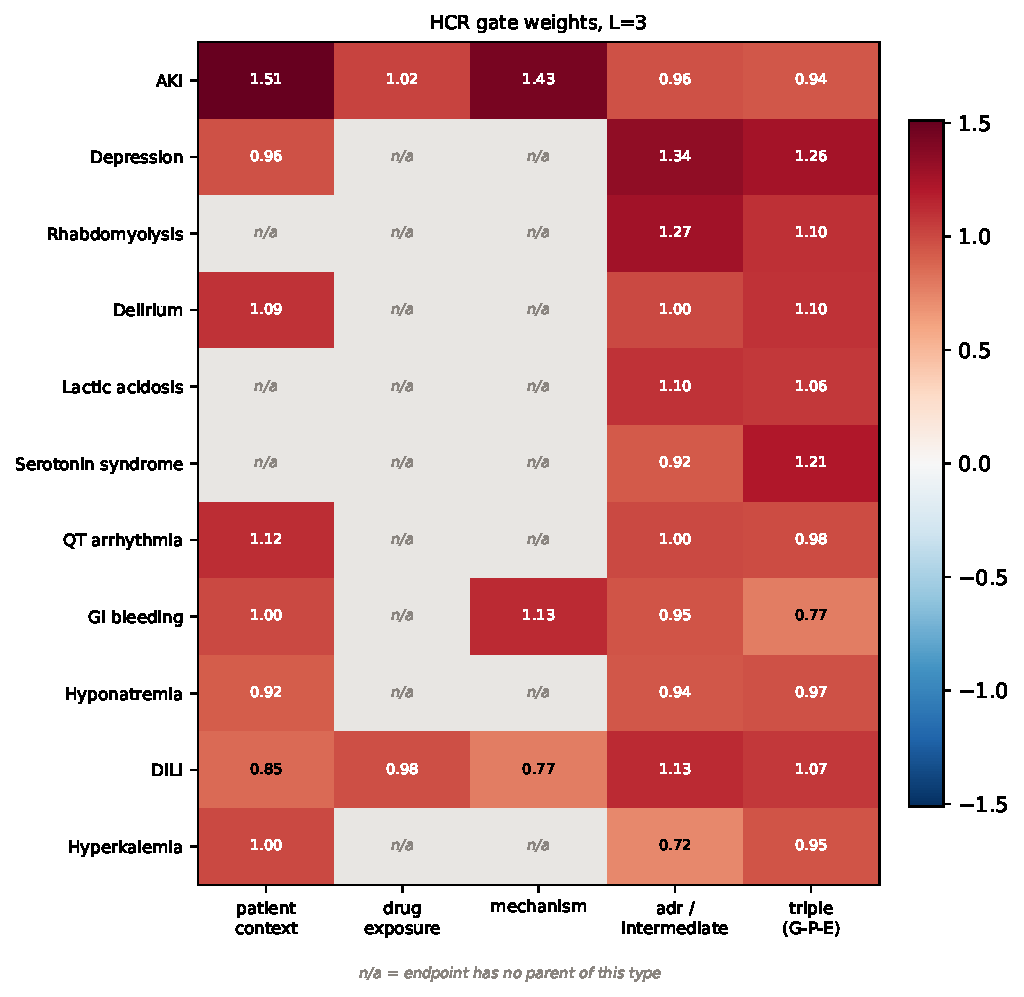
\includegraphics[width=\textwidth]{hcr_gate_matrix.pdf}
  \caption{Statistical-evidence gate matrix: influence of parent node type per endpoint.}
  \label{fig:influence}
\end{figure}

The gate ordering aligns with the number of endpoints that
have at least one direct parent of each type in the graph,
suggesting that the model allocates more weight to parent types
that are structurally more informative.

\subsection{Final Evaluation}
\label{sec:taskB-final}

In summary, models with a statistical evidence branch reached results
comparable to models with residual connections applied. 
The gate matrix indicates that the evidence branch is used
unevenly across endpoints and parent types, in line with differences in
parent availability and predictive utility on the synthetic task. 
In general the value of the statistical evidence branch therefore does not lie in raising the peak, but
in bringing stability to learning across all depths and additional information useful for clinical
event prediction.
Across the six depths evaluated, \emph{typed+triple} is the only variant that
never collapses, retaining between $82\%$ and $89\%$ of the oracle AUROC, while
both the baseline and \emph{nonlin.\ all 42D} fall below $80.00\%$ at $L=6$. 
The configuration \emph{typed+triple} is mostly stable on depth
and additionally brings the most informative value.
The highest validation score in \cref{tab:hcr-nores} is obtained by
\emph{typed+triple} at $L=1$ and $L=4$ ($89.05\%$ and $86.65\%$ of the oracle AUROC). 
Taken together, the \emph{typed+triple} statistical-evidence variant is selected as the preferred configuration.

In \cref{tab:per-endpoint} there are presented results per endpoint.

    \begin{table}[H]
      \centering
      \small
      \setlength{\tabcolsep}{4pt}
      \caption{Task~B: per-endpoint results for the selected model
        (\emph{typed+triple} at $L=4$ without residual connections).}
      \label{tab:per-endpoint}
      \begin{tabular}{lccc ccc ccc}
        \toprule
        & & \multicolumn{2}{c}{Oracle} & \multicolumn{3}{c}{Validation} & \multicolumn{3}{c}{Test} \\
        \cmidrule(lr){3-4}\cmidrule(lr){5-7}\cmidrule(lr){8-10}
        Endpoint & Prev. & AUROC & AP & AUROC & AP & \%~oracle & AUROC & AP & \%~oracle \\
        \midrule
        AKI                & 0.131 & 0.811 & 0.454 & 0.794 & 0.406 & 94.3  & 0.785 & 0.421 & 91.6 \\
        Depression         & 0.085 & 0.652 & 0.166 & 0.655 & 0.165 & 101.6 & 0.639 & 0.170 & 91.0 \\
        Hyponatremia       & 0.079 & 0.638 & 0.168 & 0.613 & 0.132 & 81.5  & 0.607 & 0.142 & 77.5 \\
        Hyperkalemia       & 0.049 & 0.590 & 0.083 & 0.595 & 0.080 & 105.7 & 0.550 & 0.074 & 55.2 \\
        Delirium           & 0.037 & 0.668 & 0.100 & 0.649 & 0.093 & 89.0  & 0.687 & 0.098 & 93.0 \\
        GI bleeding        & 0.021 & 0.570 & 0.080 & 0.570 & 0.080 & 99.0  & 0.528 & 0.029 & 39.6 \\
        DILI               & 0.018 & 0.653 & 0.086 & 0.563 & 0.067 & 41.3  & 0.579 & 0.036 & 51.6 \\
        QT arrhythmia      & 0.016 & 0.622 & 0.075 & 0.591 & 0.050 & 74.1  & 0.536 & 0.019 & 29.4 \\
        \midrule
        \textbf{Macro}     & 0.055 & 0.651 & 0.151 & 0.629 & 0.134 & 85.4  & 0.614 & 0.124 & 75.5 \\
        \midrule
        \multicolumn{10}{l}{\emph{Trained but excluded from the macro average}} \\
        Lactic acidosis    & 0.0057 & 0.523 & 0.011 & 0.560 & 0.009 & {--} & 0.549 & 0.008 & {--} \\
        Rhabdomyolysis     & 0.0037 & 0.530 & 0.011 & 0.536 & 0.005 & {--} & 0.724 & 0.033 & {--} \\
        Serotonin syndrome & 0.0027 & 0.554 & 0.008 & 0.646 & 0.010 & {--} & 0.642 & 0.008 & {--} \\
        \bottomrule
      \end{tabular}
    \end{table}

\chapter{Cross-Domain Validation of Task B. Hetionet Proxy}
\label{ch:taskB-benchmark}
\label{subsec:benchmark-endpoint}

\section{Problem Formulation and Proxy Construction}
\label{sec:hetionet-problem}

Task~B is evaluated on a benchmark dataset derived from Hetionet~\cite{hetionet}. 
Hetionet is a heterogeneous network
(\emph{hetnet}) that integrates biomedical knowledge from 29 publicly
available resources. It represents biological and pharmacological entities
as nodes and documented relationships between them as typed edges.

Hetionet v1.0 contains 47{,}031 nodes belonging to 11 node types and
2{,}250{,}197 relationships of 24 types~\cite{himmelstein2017hetionet}. The graph includes compounds,
diseases, genes, anatomies, pathways, biological processes, molecular
functions, cellular components, pharmacologic classes, side effects, and
symptoms. This heterogeneous structure makes Hetionet suitable for node classification task described further. 
The proxy construction and experimental protocol are specified in the remainder of this chapter.

\begin{figure}[H]
    \centering
    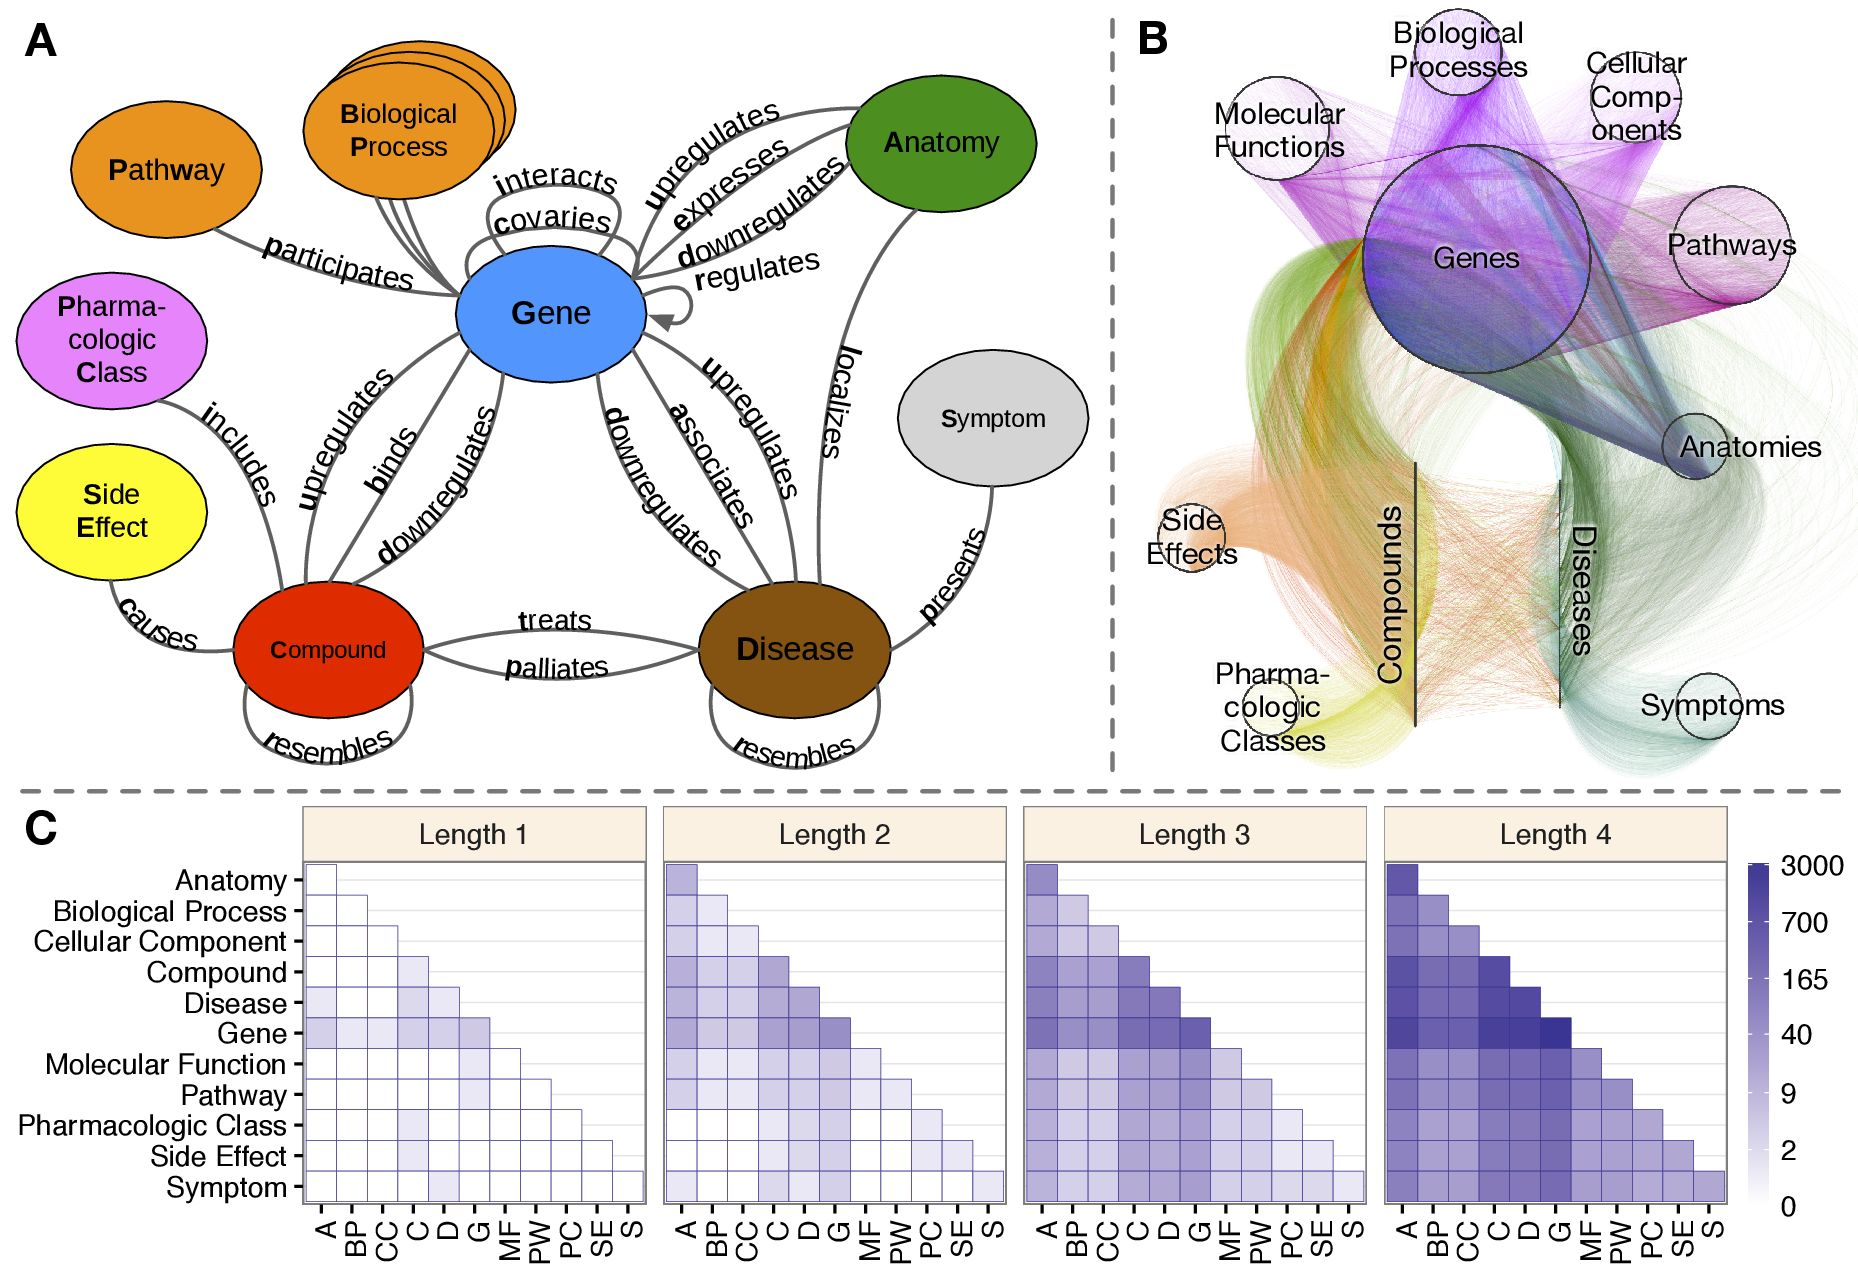
\includegraphics[width=\textwidth,keepaspectratio]{elife-26726-fig1-v2.jpg}
    \caption{Hetionet v1.0 knowledge graph (adapted from~\cite{himmelstein2017hetionet}).}
    \label{fig:hetionet-original}
\end{figure}
Figure~\ref{fig:hetionet-original} shows the Hetionet v1.0 network structure.
Hetionet was selected because it is heterogeneous and supports a
multi-label prediction setup analogous to the synthetic
task.

\section{Data Representation}
\label{sec:hetionet-data}

The
benchmark on this dataset is a structural proxy---the
pipeline, layer slots, and statistical evidence branch are reused, but the graph is
reconstructed to resemble the synthetic schema in topology. 
The reconstruction proceeds as follows. 

\begin{enumerate}[label=(\roman*)]
  \item \textbf{Instance.} A compound takes the role of the patient: the
    topology is shared and a compound is described by the edges linking it to
    the remaining entities. A compound is therefore \emph{not} a node of the
    graph, which means an entity can serve as a feature column only if it
    connects to compounds directly.

  \item \textbf{Target.} The predicted endpoint is a disease node, labelled positive when a
  \texttt{treats} or \texttt{palliates} edge links the compound to that disease
  (the two relations were merged).
  Prevalences range from $1.29\%$ to $4.51\%$ over the twenty most frequent
  diseases. 

  \item \textbf{Layer mapping.} Node types were mapped onto the slots of the
    synthetic schema as presented in \cref{tab:hetionet-mapping}.

  \item \textbf{Direction.} Hetionet edges are undirected associations.
    For pipeline compatibility, every retained edge was oriented from the
    lower to the higher synthetic layer and intra-layer edges were
    discarded, guaranteeing acyclicity. 

  \item \textbf{Path length.} Two changes lengthen the paths to a disease. First, a pathway and
  biological-process layer was inserted as the third layer, while the direct
  \texttt{DaG} edges were kept. Second, class-to-gene edges were added, because
  pharmacologic classes connect only to compounds in Hetionet and would otherwise
  have no edges at all. Such an edge is created when at least three training
  compounds of a class bind the same gene.

\end{enumerate}

% =====================================================================
%  Mapping of Hetionet node types onto the layers of the synthetic schema.
%  PREAMBLE: \usepackage{booktabs}\usepackage{tabularx}\usepackage{array}
% =====================================================================
\begin{table}[H]
  \centering
  \small
  \caption{Mapping of Hetionet entities onto the synthetic layer schema.}
  \label{tab:hetionet-mapping}
  \begin{tabular}{clll}
    \toprule
    Layer & Slot & Hetionet entity & Observed \\
    \midrule
    1 & \texttt{patient\_context}            & Pharmacologic Class (filtered)   & yes \\
    2 & \texttt{drug\_exposure}              & Gene, bound (\texttt{CbG})       & yes \\
    3 & \texttt{mechanism}                   & Pathway, Biological Process      & no (latent) \\
    4 & \texttt{adr\_or\_intermediate\_state} & Gene, associated (\texttt{DaG}) & no (latent) \\
    5 & \texttt{clinical\_endpoint}          & Disease                          & target \\
    \bottomrule
  \end{tabular}
\end{table}

Figure~\ref{fig:updated_hetionet} shows the updated layer mapping. 

\begin{figure}[H]
  \centering
  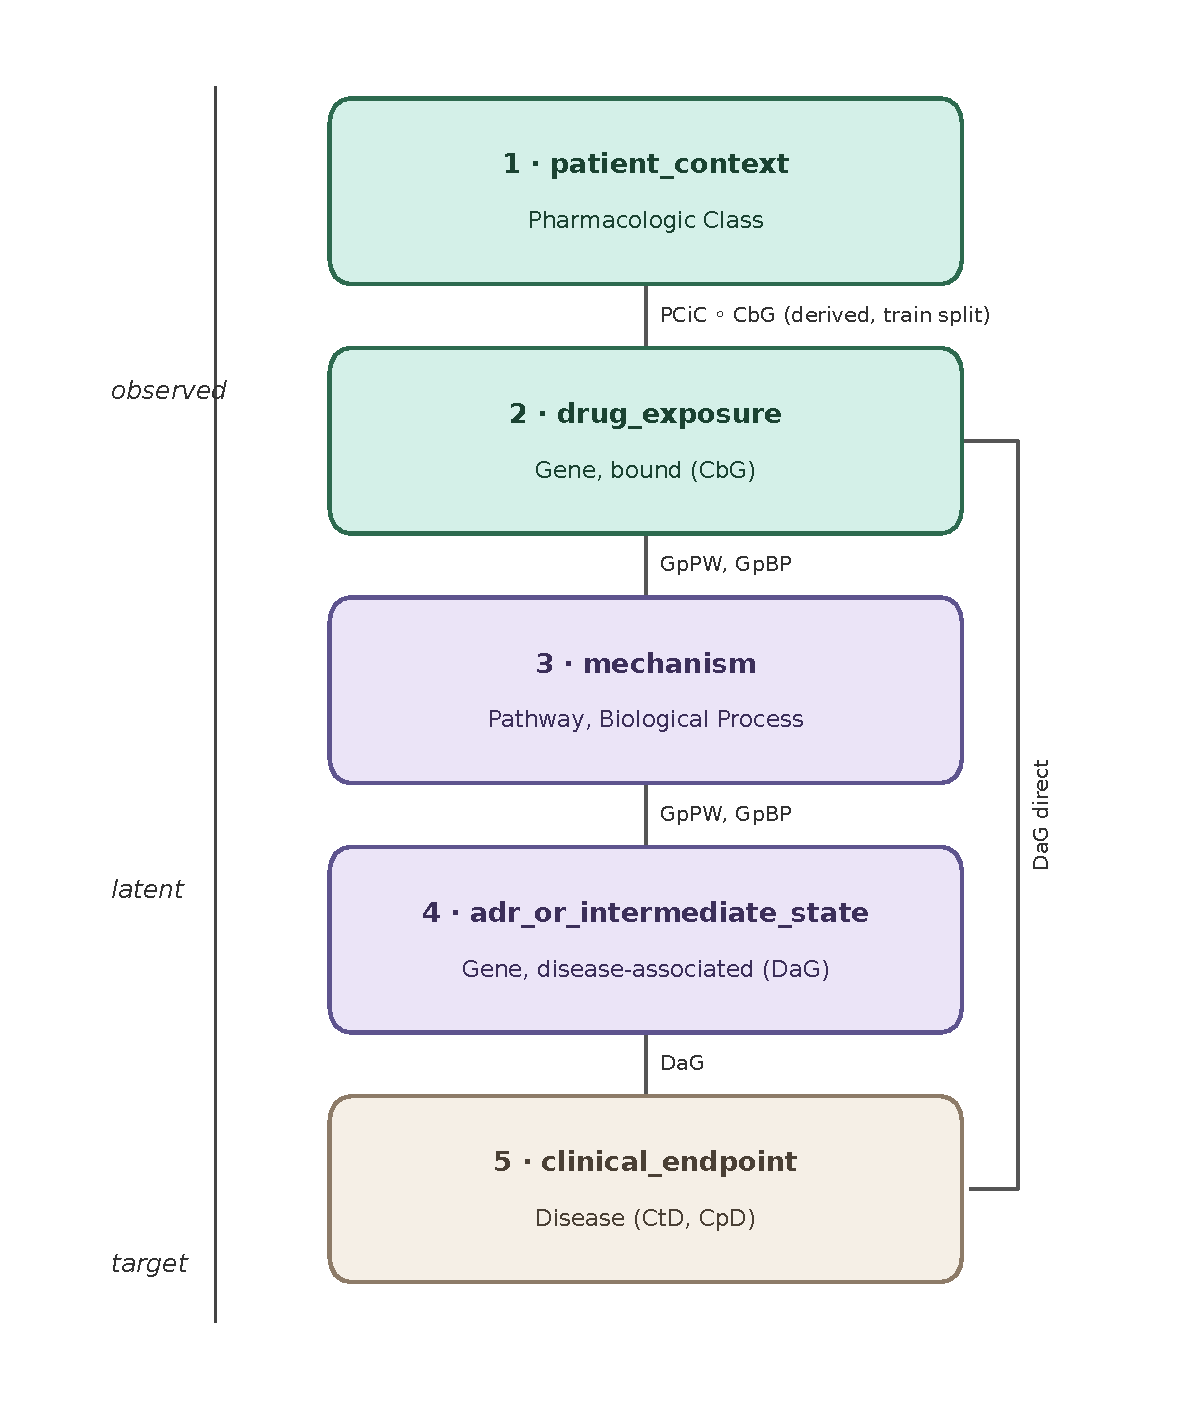
\includegraphics[width=0.78\textwidth,keepaspectratio]{hetionet_layer_mapping.pdf}
  \caption{Hetionet layer mapping after reconstruction onto the synthetic schema.}
  \label{fig:updated_hetionet}
\end{figure}

\section{Training and Evaluation}
\label{sec:hetionet-protocol}

The Hetionet proxy reuses the Task~B pipeline, layer slots, and statistical evidence branch.
Experiments use the TransformerConv backbone with hidden width $64$, batch size $8$, learning rate $1\times10^{-3}$, DropEdge disabled, and three random seeds ($42$, $20256$, $202567$).
The proxy cut comprises $1{,}552$ compounds and twenty disease endpoints.
Model selection follows the same validation-driven protocol as on the synthetic Task~B cohort.

\begin{table}[H]
  \centering
  \small
  \caption{Hetionet proxy: model and training configuration
    (differences from the Task~B synthetic protocol).}
  \label{tab:hetionet-config}
  \begin{tabular}{ll}
    \toprule
    Setting & Value \\
    \midrule
    Backbone & TransformerConv (as in Task~B) \\
    Hidden width & 64 \\
    Batch size & 8 \\
    Learning rate & $1\times10^{-3}$ \\
    DropEdge & disabled \\
    Seeds & $42$, $20256$, $202567$ \\
    Compounds (instances) & $1{,}552$ \\
    Disease endpoints & 20 \\
    \bottomrule
  \end{tabular}
\end{table}

\section{Experimental Results}
\label{sec:hetionet-results}

% The models on benchmark dataset shows the same trend as on synthethic dataset. 
% The approach with HCR significantly improves results comparing to baseline model without HCR. 
% It generates similar results as models with residual connections, but what it is interesting on the benchamrk dataset
% HCR combined with residual connections reaches the higher results than separated approach. 

The benchmark reproduces several trends
observed on the synthetic dataset -- depth sensitivity without stabilisers,
partial recovery with the statistical evidence branch -- under a different graph semantics 
and without
oracle metrics.
Reported scores in \cref{tab:proxy-full} are the mean $\pm$ sample standard deviation
over up to three seeds.
The gain from statistical evidence is conditional on the state of the
propagation path: at $L=6$ without residual connections the graph-only model
reaches $0.615 \pm 0.026$ test AUROC, while statistical-evidence variants recover
part of the lost ranking quality ($0.703$--$0.712$).
At $L=1$, where the receptive field of an endpoint coincides with the input of
the statistical evidence branch, graph-only and statistical-evidence variants remain close
(test AUROC $0.667$--$0.672$).

At $L=6$, residual connections already restore much of the graph pathway
($0.728 \pm 0.010$ without the statistical branch).
Adding statistical evidence on top of residuals yields $0.726$--$0.742$, so the
two mechanisms are only weakly additive on this proxy: the residual path carries
most of the depth-related gain, while the statistical branch helps mainly when
that path is absent.

The reason is the structure of the two graphs. In the synthetic graph the direct
parents of an endpoint are observed, so the statistical evidence branch and the one-hop
receptive field read the same variables and the two mechanisms address the same
bottleneck. In the Hetionet-derived graph depth is more crucial because some
layers are latent. Information must
therefore traverse several hops, and the residual path and the HCR bypass
contribute at different points of that route.

Overall, the proxy experiment suggests that combining message passing
with the statistical evidence branch remains useful with 
multi-hop reasoning. Whether an
additional residual path helps or hinders depends on where 
the statistical
evidence enters the model.

% =====================================================================
%  PROXY DATASET RESULTS (Hetionet, cut A, proxy3_clean)
%  seeds 42 + 20256 + 202567; mean ± sample SD; n=3 unless noted
% =====================================================================
\begin{table}[H]
  \centering
  \scriptsize
  \setlength{\tabcolsep}{3pt}
  \caption{Hetionet proxy: endpoint-prediction results under the reconstructed layer schema.}
  \label{tab:proxy-full}
  \resizebox{\textwidth}{!}{%
  \begin{tabular}{ccl ccc ccc}
    \toprule
    & & & \multicolumn{3}{c}{Validation} & \multicolumn{3}{c}{Test} \\
    \cmidrule(lr){4-6}\cmidrule(lr){7-9}
    $L$ & Res. & Evidence variant & {AUROC} & {AP} & {Lift} & {AUROC} & {AP} & {Lift} \\
    \midrule
    1 & no  & ---              & $0.757{\scriptstyle\,\pm\,0.005}$ & $0.218{\scriptstyle\,\pm\,0.027}$ & $9.20{\scriptstyle\,\pm\,1.15}$ & $0.668{\scriptstyle\,\pm\,0.006}$ & $0.125{\scriptstyle\,\pm\,0.010}$ & $6.78{\scriptstyle\,\pm\,0.53}$ \\
    1 & no  & nonlin.\ bin.    & $0.758{\scriptstyle\,\pm\,0.005}$ & $0.219{\scriptstyle\,\pm\,0.020}$ & $9.23{\scriptstyle\,\pm\,0.83}$ & $0.667{\scriptstyle\,\pm\,0.008}$ & $0.128{\scriptstyle\,\pm\,0.007}$ & $6.90{\scriptstyle\,\pm\,0.39}$ \\
    1 & no  & nonlin.\ all     & $0.757{\scriptstyle\,\pm\,0.004}$ & $0.213{\scriptstyle\,\pm\,0.012}$ & $8.99{\scriptstyle\,\pm\,0.52}$ & $0.667{\scriptstyle\,\pm\,0.002}$ & $0.135{\scriptstyle\,\pm\,0.005}$ & $7.27{\scriptstyle\,\pm\,0.24}$ \\
    1 & no  & typed+triple     & $0.765{\scriptstyle\,\pm\,0.011}$ & $0.216{\scriptstyle\,\pm\,0.049}$ & $9.10{\scriptstyle\,\pm\,2.05}$ & $0.668{\scriptstyle\,\pm\,0.006}$ & $0.132{\scriptstyle\,\pm\,0.026}$ & $7.17{\scriptstyle\,\pm\,1.40}$ \\
    \addlinespace[2pt]
    1 & yes & ---              & $0.756{\scriptstyle\,\pm\,0.002}$ & $0.213{\scriptstyle\,\pm\,0.014}$ & $8.96{\scriptstyle\,\pm\,0.61}$ & $0.671{\scriptstyle\,\pm\,0.004}$ & $0.132{\scriptstyle\,\pm\,0.029}$ & $7.13{\scriptstyle\,\pm\,1.55}$ \\
    1 & yes & nonlin.\ bin.    & $0.756{\scriptstyle\,\pm\,0.005}$ & $0.215{\scriptstyle\,\pm\,0.019}$ & $9.06{\scriptstyle\,\pm\,0.81}$ & $0.672{\scriptstyle\,\pm\,0.007}$ & $0.142{\scriptstyle\,\pm\,0.006}$ & $7.69{\scriptstyle\,\pm\,0.35}$ \\
    1 & yes & nonlin.\ all     & $0.757{\scriptstyle\,\pm\,0.001}$ & $0.222{\scriptstyle\,\pm\,0.018}$ & $9.38{\scriptstyle\,\pm\,0.77}$ & $0.667{\scriptstyle\,\pm\,0.003}$ & $0.137{\scriptstyle\,\pm\,0.002}$ & $7.41{\scriptstyle\,\pm\,0.08}$ \\
    1 & yes & typed+triple     & $0.755{\scriptstyle\,\pm\,0.004}$ & $0.210{\scriptstyle\,\pm\,0.046}$ & $8.84{\scriptstyle\,\pm\,1.94}$ & $0.671{\scriptstyle\,\pm\,0.009}$ & $0.136{\scriptstyle\,\pm\,0.034}$ & $7.37{\scriptstyle\,\pm\,1.83}$ \\
    \midrule
    %2 & no  & ---$^*$          & $0.754{\scriptstyle\,\pm\,0.002}$ & $0.234{\scriptstyle\,\pm\,0.005}$ & $9.87{\scriptstyle\,\pm\,0.21}$ & $0.686{\scriptstyle\,\pm\,0.006}$ & $0.118{\scriptstyle\,\pm\,0.015}$ & $6.38{\scriptstyle\,\pm\,0.82}$ \\
    2 & no  & nonlin.\ bin.$^*$ & $0.761{\scriptstyle\,\pm\,0.004}$ & $0.254{\scriptstyle\,\pm\,0.000}$ & $10.70{\scriptstyle\,\pm\,0.01}$ & $0.683{\scriptstyle\,\pm\,0.007}$ & $0.160{\scriptstyle\,\pm\,0.004}$ & $8.66{\scriptstyle\,\pm\,0.20}$ \\
    2 & no  & nonlin.\ all     & $0.760{\scriptstyle\,\pm\,0.005}$ & $0.261{\scriptstyle\,\pm\,0.018}$ & $11.03{\scriptstyle\,\pm\,0.75}$ & $0.686{\scriptstyle\,\pm\,0.009}$ & $0.165{\scriptstyle\,\pm\,0.029}$ & $8.93{\scriptstyle\,\pm\,1.56}$ \\
    2 & no  & typed+triple     & $0.768{\scriptstyle\,\pm\,0.008}$ & $0.262{\scriptstyle\,\pm\,0.002}$ & $11.06{\scriptstyle\,\pm\,0.07}$ & $0.685{\scriptstyle\,\pm\,0.007}$ & $0.169{\scriptstyle\,\pm\,0.005}$ & $9.14{\scriptstyle\,\pm\,0.28}$ \\
    \addlinespace[2pt]
    %2 & yes & ---$^*$          & $0.756{\scriptstyle\,\pm\,0.003}$ & $0.247{\scriptstyle\,\pm\,0.008}$ & $10.40{\scriptstyle\,\pm\,0.36}$ & $0.685{\scriptstyle\,\pm\,0.004}$ & $0.153{\scriptstyle\,\pm\,0.046}$ & $8.26{\scriptstyle\,\pm\,2.49}$ \\
    2 & yes & nonlin.\ bin.$^*$ & $0.764{\scriptstyle\,\pm\,0.004}$ & $0.277{\scriptstyle\,\pm\,0.004}$ & $11.70{\scriptstyle\,\pm\,0.17}$ & $0.691{\scriptstyle\,\pm\,0.009}$ & $0.181{\scriptstyle\,\pm\,0.011}$ & $9.78{\scriptstyle\,\pm\,0.58}$ \\
    2 & yes & nonlin.\ all     & $0.758{\scriptstyle\,\pm\,0.003}$ & $0.241{\scriptstyle\,\pm\,0.015}$ & $10.15{\scriptstyle\,\pm\,0.62}$ & $0.685{\scriptstyle\,\pm\,0.004}$ & $0.162{\scriptstyle\,\pm\,0.007}$ & $8.75{\scriptstyle\,\pm\,0.39}$ \\
    2 & yes & typed+triple     & $0.768{\scriptstyle\,\pm\,0.004}$ & $0.258{\scriptstyle\,\pm\,0.022}$ & $10.86{\scriptstyle\,\pm\,0.93}$ & $0.691{\scriptstyle\,\pm\,0.001}$ & $0.189{\scriptstyle\,\pm\,0.014}$ & $10.21{\scriptstyle\,\pm\,0.75}$ \\
    \midrule
    3 & no  & ---              & $0.742{\scriptstyle\,\pm\,0.012}$ & $0.200{\scriptstyle\,\pm\,0.008}$ & $8.45{\scriptstyle\,\pm\,0.35}$ & $0.689{\scriptstyle\,\pm\,0.029}$ & $0.132{\scriptstyle\,\pm\,0.027}$ & $7.13{\scriptstyle\,\pm\,1.46}$ \\
    3 & no  & nonlin.\ bin.    & $0.798{\scriptstyle\,\pm\,0.009}$ & $0.275{\scriptstyle\,\pm\,0.003}$ & $11.59{\scriptstyle\,\pm\,0.13}$ & $0.692{\scriptstyle\,\pm\,0.008}$ & $0.172{\scriptstyle\,\pm\,0.005}$ & $9.28{\scriptstyle\,\pm\,0.28}$ \\
    3 & no  & nonlin.\ all     & $0.791{\scriptstyle\,\pm\,0.016}$ & $0.264{\scriptstyle\,\pm\,0.006}$ & $11.13{\scriptstyle\,\pm\,0.24}$ & $0.700{\scriptstyle\,\pm\,0.002}$ & $0.165{\scriptstyle\,\pm\,0.001}$ & $8.91{\scriptstyle\,\pm\,0.08}$ \\
    3 & no  & typed+triple     & $0.801{\scriptstyle\,\pm\,0.006}$ & $0.266{\scriptstyle\,\pm\,0.025}$ & $11.23{\scriptstyle\,\pm\,1.06}$ & $0.702{\scriptstyle\,\pm\,0.002}$ & $0.167{\scriptstyle\,\pm\,0.001}$ & $9.05{\scriptstyle\,\pm\,0.06}$ \\
    \addlinespace[2pt]
    3 & yes & ---              & $0.802{\scriptstyle\,\pm\,0.004}$ & $0.270{\scriptstyle\,\pm\,0.045}$ & $11.41{\scriptstyle\,\pm\,1.90}$ & $0.700{\scriptstyle\,\pm\,0.014}$ & $0.179{\scriptstyle\,\pm\,0.014}$ & $9.70{\scriptstyle\,\pm\,0.76}$ \\
    3 & yes & nonlin.\ bin.    & $0.799{\scriptstyle\,\pm\,0.020}$ & $0.270{\scriptstyle\,\pm\,0.036}$ & $11.40{\scriptstyle\,\pm\,1.54}$ & $0.712{\scriptstyle\,\pm\,0.003}$ & $0.179{\scriptstyle\,\pm\,0.023}$ & $9.67{\scriptstyle\,\pm\,1.25}$ \\
    3 & yes & nonlin.\ all     & $0.805{\scriptstyle\,\pm\,0.004}$ & $0.274{\scriptstyle\,\pm\,0.013}$ & $11.54{\scriptstyle\,\pm\,0.54}$ & $0.696{\scriptstyle\,\pm\,0.017}$ & $0.177{\scriptstyle\,\pm\,0.005}$ & $9.59{\scriptstyle\,\pm\,0.30}$ \\
    3 & yes & typed+triple     & $0.803{\scriptstyle\,\pm\,0.003}$ & $0.289{\scriptstyle\,\pm\,0.036}$ & $12.20{\scriptstyle\,\pm\,1.52}$ & $0.711{\scriptstyle\,\pm\,0.004}$ & $0.185{\scriptstyle\,\pm\,0.006}$ & $10.00{\scriptstyle\,\pm\,0.34}$ \\
    \midrule
    %4 & no  & ---$^*$          & $0.610{\scriptstyle\,\pm\,0.008}$ & $0.133{\scriptstyle\,\pm\,0.000}$ & $5.60{\scriptstyle\,\pm\,0.01}$ & $0.624{\scriptstyle\,\pm\,0.003}$ & $0.078{\scriptstyle\,\pm\,0.003}$ & $4.20{\scriptstyle\,\pm\,0.14}$ \\
    4 & no  & nonlin.\ bin.$^*$ & $0.760{\scriptstyle\,\pm\,0.001}$ & $0.254{\scriptstyle\,\pm\,0.005}$ & $10.71{\scriptstyle\,\pm\,0.20}$ & $0.683{\scriptstyle\,\pm\,0.006}$ & $0.169{\scriptstyle\,\pm\,0.002}$ & $9.13{\scriptstyle\,\pm\,0.12}$ \\
    4 & no  & nonlin.\ all     & $0.774{\scriptstyle\,\pm\,0.016}$ & $0.237{\scriptstyle\,\pm\,0.006}$ & $9.99{\scriptstyle\,\pm\,0.26}$ & $0.702{\scriptstyle\,\pm\,0.022}$ & $0.152{\scriptstyle\,\pm\,0.001}$ & $8.21{\scriptstyle\,\pm\,0.06}$ \\
    4 & no  & typed+triple     & $0.778{\scriptstyle\,\pm\,0.025}$ & $0.264{\scriptstyle\,\pm\,0.004}$ & $11.12{\scriptstyle\,\pm\,0.17}$ & $0.708{\scriptstyle\,\pm\,0.033}$ & $0.172{\scriptstyle\,\pm\,0.008}$ & $9.30{\scriptstyle\,\pm\,0.46}$ \\
    \addlinespace[2pt]
    %4 & yes & ---$^*$          & $0.804{\scriptstyle\,\pm\,0.002}$ & $0.266{\scriptstyle\,\pm\,0.010}$ & $11.20{\scriptstyle\,\pm\,0.42}$ & $0.711{\scriptstyle\,\pm\,0.014}$ & $0.176{\scriptstyle\,\pm\,0.020}$ & $9.51{\scriptstyle\,\pm\,1.10}$ \\
    4 & yes & nonlin.\ bin.$^*$ & $0.815{\scriptstyle\,\pm\,0.003}$ & $0.297{\scriptstyle\,\pm\,0.002}$ & $12.52{\scriptstyle\,\pm\,0.09}$ & $0.729{\scriptstyle\,\pm\,0.007}$ & $0.198{\scriptstyle\,\pm\,0.001}$ & $10.70{\scriptstyle\,\pm\,0.03}$ \\
    4 & yes & nonlin.\ all     & $0.798{\scriptstyle\,\pm\,0.022}$ & $0.264{\scriptstyle\,\pm\,0.022}$ & $11.14{\scriptstyle\,\pm\,0.94}$ & $0.709{\scriptstyle\,\pm\,0.015}$ & $0.188{\scriptstyle\,\pm\,0.022}$ & $10.16{\scriptstyle\,\pm\,1.18}$ \\
    4 & yes & typed+triple     & $0.808{\scriptstyle\,\pm\,0.008}$ & $0.285{\scriptstyle\,\pm\,0.039}$ & $12.03{\scriptstyle\,\pm\,1.67}$ & $0.737{\scriptstyle\,\pm\,0.023}$ & $0.185{\scriptstyle\,\pm\,0.015}$ & $9.99{\scriptstyle\,\pm\,0.85}$ \\
    \midrule
    5 & no  & ---$^*$          & $0.605{\scriptstyle\,\pm\,0.000}$ & $0.133{\scriptstyle\,\pm\,0.004}$ & $5.63{\scriptstyle\,\pm\,0.16}$ & $0.628{\scriptstyle\,\pm\,0.001}$ & $0.083{\scriptstyle\,\pm\,0.005}$ & $4.50{\scriptstyle\,\pm\,0.27}$ \\
    5 & no  & nonlin.\ bin.$^*$ & $0.796{\scriptstyle\,\pm\,0.000}$ & $0.249{\scriptstyle\,\pm\,0.003}$ & $10.50{\scriptstyle\,\pm\,0.11}$ & $0.751{\scriptstyle\,\pm\,0.002}$ & $0.161{\scriptstyle\,\pm\,0.001}$ & $8.72{\scriptstyle\,\pm\,0.03}$ \\
    5 & no  & nonlin.\ all     & $0.775{\scriptstyle\,\pm\,0.017}$ & $0.241{\scriptstyle\,\pm\,0.002}$ & $10.15{\scriptstyle\,\pm\,0.07}$ & $0.693{\scriptstyle\,\pm\,0.021}$ & $0.159{\scriptstyle\,\pm\,0.007}$ & $8.59{\scriptstyle\,\pm\,0.36}$ \\
    5 & no  & typed+triple     & $0.792{\scriptstyle\,\pm\,0.013}$ & $0.262{\scriptstyle\,\pm\,0.016}$ & $11.06{\scriptstyle\,\pm\,0.69}$ & $0.714{\scriptstyle\,\pm\,0.038}$ & $0.165{\scriptstyle\,\pm\,0.002}$ & $8.92{\scriptstyle\,\pm\,0.12}$ \\
    \addlinespace[2pt]
    5 & yes & ---$^*$          & $0.807{\scriptstyle\,\pm\,0.008}$ & $0.293{\scriptstyle\,\pm\,0.015}$ & $12.36{\scriptstyle\,\pm\,0.63}$ & $0.735{\scriptstyle\,\pm\,0.021}$ & $0.190{\scriptstyle\,\pm\,0.002}$ & $10.29{\scriptstyle\,\pm\,0.10}$ \\
    5 & yes & nonlin.\ bin.$^*$ & $0.816{\scriptstyle\,\pm\,0.003}$ & $0.326{\scriptstyle\,\pm\,0.017}$ & $13.76{\scriptstyle\,\pm\,0.73}$ & $0.763{\scriptstyle\,\pm\,0.020}$ & $0.212{\scriptstyle\,\pm\,0.025}$ & $11.49{\scriptstyle\,\pm\,1.37}$ \\
    5 & yes & nonlin.\ all     & $0.812{\scriptstyle\,\pm\,0.004}$ & $0.299{\scriptstyle\,\pm\,0.008}$ & $12.60{\scriptstyle\,\pm\,0.31}$ & $0.728{\scriptstyle\,\pm\,0.001}$ & $0.179{\scriptstyle\,\pm\,0.009}$ & $9.67{\scriptstyle\,\pm\,0.48}$ \\
    5 & yes & typed+triple     & $0.820{\scriptstyle\,\pm\,0.010}$ & $0.292{\scriptstyle\,\pm\,0.023}$ & $12.29{\scriptstyle\,\pm\,0.97}$ & $0.731{\scriptstyle\,\pm\,0.014}$ & $0.197{\scriptstyle\,\pm\,0.021}$ & $10.67{\scriptstyle\,\pm\,1.13}$ \\
    \midrule
    6 & no  & ---              & $0.608{\scriptstyle\,\pm\,0.002}$ & $0.128{\scriptstyle\,\pm\,0.006}$ & $5.40{\scriptstyle\,\pm\,0.25}$ & $0.615{\scriptstyle\,\pm\,0.026}$ & $0.079{\scriptstyle\,\pm\,0.002}$ & $4.27{\scriptstyle\,\pm\,0.11}$ \\
    6 & no  & nonlin.\ bin.    & $0.782{\scriptstyle\,\pm\,0.013}$ & $0.237{\scriptstyle\,\pm\,0.023}$ & $9.98{\scriptstyle\,\pm\,0.97}$ & $0.707{\scriptstyle\,\pm\,0.038}$ & $0.165{\scriptstyle\,\pm\,0.009}$ & $8.94{\scriptstyle\,\pm\,0.48}$ \\
    6 & no  & nonlin.\ all     & $0.771{\scriptstyle\,\pm\,0.028}$ & $0.239{\scriptstyle\,\pm\,0.005}$ & $10.07{\scriptstyle\,\pm\,0.23}$ & $0.703{\scriptstyle\,\pm\,0.020}$ & $0.153{\scriptstyle\,\pm\,0.004}$ & $8.29{\scriptstyle\,\pm\,0.20}$ \\
    6 & no  & typed+triple     & $0.777{\scriptstyle\,\pm\,0.022}$ & $0.261{\scriptstyle\,\pm\,0.002}$ & $11.01{\scriptstyle\,\pm\,0.09}$ & $0.712{\scriptstyle\,\pm\,0.039}$ & $0.167{\scriptstyle\,\pm\,0.007}$ & $9.05{\scriptstyle\,\pm\,0.35}$ \\
    \addlinespace[2pt]
    6 & yes & ---              & $0.811{\scriptstyle\,\pm\,0.006}$ & $0.263{\scriptstyle\,\pm\,0.029}$ & $11.11{\scriptstyle\,\pm\,1.20}$ & $0.728{\scriptstyle\,\pm\,0.010}$ & $0.168{\scriptstyle\,\pm\,0.022}$ & $9.09{\scriptstyle\,\pm\,1.20}$ \\
    6 & yes & nonlin.\ bin.    & $0.820{\scriptstyle\,\pm\,0.011}$ & $0.302{\scriptstyle\,\pm\,0.023}$ & $12.74{\scriptstyle\,\pm\,0.97}$ & $0.742{\scriptstyle\,\pm\,0.016}$ & $0.186{\scriptstyle\,\pm\,0.015}$ & $10.06{\scriptstyle\,\pm\,0.81}$ \\
    6 & yes & nonlin.\ all     & $0.814{\scriptstyle\,\pm\,0.005}$ & $0.278{\scriptstyle\,\pm\,0.037}$ & $11.71{\scriptstyle\,\pm\,1.56}$ & $0.739{\scriptstyle\,\pm\,0.009}$ & $0.180{\scriptstyle\,\pm\,0.014}$ & $9.71{\scriptstyle\,\pm\,0.76}$ \\
    6 & yes & typed+triple     & $0.815{\scriptstyle\,\pm\,0.006}$ & $0.298{\scriptstyle\,\pm\,0.042}$ & $12.57{\scriptstyle\,\pm\,1.78}$ & $0.726{\scriptstyle\,\pm\,0.010}$ & $0.204{\scriptstyle\,\pm\,0.007}$ & $11.05{\scriptstyle\,\pm\,0.38}$ \\
    \bottomrule
  \end{tabular}%
  }
\end{table}

% ---------------------------------------------------------------------
% TABLE 1 - full observability regime
% ---------------------------------------------------------------------
% \begin{table}[H]
%     \centering
%     \caption{Results under full observability on the proxy dataset. The
%       epoch was selected on the validation set. \texttt{---} in the HCR
%       column denotes a model without the HCR branch. Lift is AUPRC
%       divided by the prevalence baseline. Jumping knowledge was not used
%       in any configuration.}
%     \label{tab:proxy-full}
%     \sisetup{table-format=1.3}
%     \begin{tabular}{ccl SSS SSS}
%       \toprule
%       & & & \multicolumn{3}{c}{Validation} & \multicolumn{3}{c}{Test} \\
%       \cmidrule(lr){4-6}\cmidrule(lr){7-9}
%       $L$ & Residual & HCR & {AUC} & {AUPRC} & {Lift} & {AUC} & {AUPRC} & {Lift} \\
%       \midrule
%       1 & no  & ---            & 0.757 & 0.188 & 7.92  & 0.664 & 0.120 & 6.49 \\
%       1 & no  & nonlin.\ 9D    & 0.763 & 0.207 & 8.75  & 0.657 & 0.120 & 6.47 \\
%       1 & no  & typed 41D      & 0.759 & 0.194 & 8.17  & 0.663 & 0.116 & 6.29 \\
%       \addlinespace[2pt]
%       1 & yes & ---            & 0.756 & 0.196 & 8.26  & 0.669 & 0.106 & 5.72 \\
%       1 & yes & nonlin.\ 9D    & 0.756 & 0.201 & 8.49  & 0.670 & 0.135 & 7.31 \\
%       1 & yes & typed 41D      & 0.754 & 0.185 & 7.79  & 0.671 & 0.124 & 6.71 \\
%       \midrule
%       3 & no  & ---            & 0.756 & 0.199 & 8.38  & {\bfseries 0.722} & 0.152 & 8.24 \\
%       3 & no  & nonlin.\ 9D    & 0.805 & 0.275 & 11.62 & 0.686 & 0.169 & 9.14 \\
%       3 & no  & typed 41D      & 0.812 & 0.243 & 10.26 & 0.678 & 0.154 & 8.32 \\
%       \addlinespace[2pt]
%       3 & yes & ---            & 0.799 & 0.225 & 9.48  & 0.685 & 0.166 & 8.97 \\
%       3 & yes & nonlin.\ 9D    & 0.814 & 0.235 & 9.90  & 0.714 & 0.183 & 9.92 \\
%       3 & yes & typed 41D      & 0.802 & 0.255 & 10.76 & 0.678 & 0.151 & 8.16 \\
%       \midrule
%       6 & no  & ---            & 0.610 & 0.121 & 5.11  & 0.585 & 0.077 & 4.14 \\
%       6 & no  & nonlin.\ 9D    & 0.782 & 0.210 & 8.86  & 0.680 & 0.174 & 9.42 \\
%       6 & no  & typed 41D      & 0.794 & 0.235 & 9.89  & 0.680 & 0.126 & 6.84 \\
%       \addlinespace[2pt]
%       6 & yes & ---            & 0.817 & 0.255 & 10.77 & 0.728 & 0.173 & 9.36 \\
%       6 & yes & nonlin.\ 9D    & {\bfseries 0.832} & {\bfseries 0.310} & {\bfseries 13.06} & {\bfseries 0.760} & 0.179 & 9.70 \\
%       6 & yes & typed 41D      & 0.815 & 0.284 & 11.99 & 0.744 & {\bfseries 0.239} & {\bfseries 12.91} \\
%       \bottomrule
%     \end{tabular}
%   \end{table}
  
  
  % ---------------------------------------------------------------------
  % TABLE 3 - representation smoothing metrics
  % ---------------------------------------------------------------------
  % \begin{table}[H]
  %   \centering
  %   \caption{Representation smoothing metrics under full observability,
  %     measured on the validation set. By the conventional reading, lower
  %     MAD and higher cosine similarity indicate stronger smoothing.
  %     Validation AUC is repeated for comparison. Note that residual
  %     configurations appear more smoothed by every metric while
  %     performing better.}
  %   \label{tab:proxy-oversmoothing}
  %   \sisetup{table-format=1.4}
  %   \begin{tabular}{ccl SSSS S[table-format=1.3]}
  %     \toprule
  %     $L$ & Residual & HCR & {MAD} & {Cos.\ sim.} & {Cos.\ sim.\ (ep.)} & {Dirichlet} & {AUC} \\
  %     \midrule
  %     1 & no  & ---         & 0.7691 & 0.6216 & 0.8246 & 0.2706 & 0.757 \\
  %     1 & no  & nonlin.\ 9D & 0.7629 & 0.6142 & 0.7844 & 0.2495 & 0.763 \\
  %     1 & no  & typed 41D   & 0.7684 & 0.6191 & 0.8148 & 0.2706 & 0.759 \\
  %     \addlinespace[2pt]
  %     1 & yes & ---         & 0.7363 & 0.7042 & 0.7606 & 0.5724 & 0.756 \\
  %     1 & yes & nonlin.\ 9D & 0.7448 & 0.6946 & 0.7060 & 0.5048 & 0.756 \\
  %     1 & yes & typed 41D   & 0.7410 & 0.7026 & 0.7899 & 0.5022 & 0.754 \\
  %     \midrule
  %     3 & no  & ---         & 0.6515 & 0.6798 & 0.9582 & 0.1175 & 0.756 \\
  %     3 & no  & nonlin.\ 9D & 0.7067 & 0.6641 & 0.8365 & 0.0904 & 0.805 \\
  %     3 & no  & typed 41D   & 0.7235 & 0.6314 & 0.7333 & 0.0972 & 0.812 \\
  %     \addlinespace[2pt]
  %     3 & yes & ---         & 0.4842 & 0.8319 & 0.7772 & 0.3712 & 0.799 \\
  %     3 & yes & nonlin.\ 9D & 0.5517 & 0.7782 & 0.7752 & 0.3905 & 0.814 \\
  %     3 & yes & typed 41D   & 0.5113 & 0.8275 & 0.7132 & 0.4044 & 0.802 \\
  %     \midrule
  %     6 & no  & ---         & 0.7060 & 0.6530 & 0.8604 & 0.1024 & 0.610 \\
  %     6 & no  & nonlin.\ 9D & 0.7101 & 0.6495 & 0.7815 & 0.0892 & 0.782 \\
  %     6 & no  & typed 41D   & 0.7222 & 0.6408 & 0.8657 & 0.0949 & 0.794 \\
  %     \addlinespace[2pt]
  %     6 & yes & ---         & 0.5634 & 0.7975 & 0.7949 & 0.3143 & 0.817 \\
  %     6 & yes & nonlin.\ 9D & 0.5030 & 0.8174 & 0.6658 & 0.2636 & 0.832 \\
  %     6 & yes & typed 41D   & 0.5623 & 0.8095 & 0.8472 & 0.3930 & 0.815 \\
  %     \bottomrule
  %   \end{tabular}
  % \end{table}


\chapter{Discussion and Limitations}
\label{ch:joint-discussion}

\section{Common Methodological Principle}
\label{sec:joint-shared}

The two prediction tasks investigated in this thesis address different objects, but are
based on a common methodological principle: structured graph knowledge and explicit
empirical statistical evidence provide different, potentially complementary descriptions
of the same system.

In Task~A, the prediction object is a candidate directed relation. The structural branch
describes the position of the candidate nodes within the heterogeneous graph, while the
statistical branch describes empirical dependence patterns observed in the patient
population. In Task~B, the graph topology is shared across patients and the prediction
object becomes a patient-specific clinical endpoint. Patient observations are propagated
through the graph, while an explicit statistical evidence branch provides an additional
description of endpoint-related dependencies.

The common modelling template can therefore be summarized as
\begin{equation}
\text{structured graph representation}
\;+\;
\text{explicit empirical evidence}
\;\rightarrow\;
\text{task-specific prediction}.
\end{equation}
The relative contribution of the two components is task dependent. Statistical evidence is
particularly useful when relevant information is not adequately represented or preserved
by the graph pathway, whereas a sufficiently effective graph encoder may already capture
part of the same signal.
On the synthetic Task~B benchmark this distinction is concrete: when residual connections
preserve endpoint-relevant information inside the message-passing stack, the evaluated
statistical-evidence variants do not provide a consistent additional improvement over the
corresponding graph-only residual models, whereas the same branch recovers substantial
performance when deep models degrade without residual propagation.

\section{What the Two Synthetic Tasks Show}
\label{sec:joint-synthetic}

\subsection*{Task~A: confronting structured knowledge with observational evidence}

Task~A demonstrates that patient-derived statistical evidence can provide substantial
information beyond heterogeneous graph topology alone. Progressive enrichment of the
candidate-specific statistical representation improves directed edge ranking relative to the
graph-only HGT baseline.

Importantly, statistical dependence does not determine edge direction. Direction is supplied
by the ordered candidate definition and the mechanistic graph schema. HCR-derived
coefficients provide empirical evidence about relationships between variables, but are not
interpreted as causal effects.
Task~A can therefore be understood as confronting prior structured knowledge with
population-level observational evidence under a controlled reconstruction objective.
It does not perform causal discovery.

Residual connections inside the Task~A HGT encoder are standard skip connections with
LayerNorm; they are architectural details of the structural branch and are not studied as an
anti-oversmoothing intervention in that chapter.

\subsection*{Task~B: structural context for patient-level endpoints}

Task~B examines whether a shared mechanistic graph can provide useful structural context
for predicting patient-level clinical endpoints.

The experiments show that the usefulness of the statistical branch depends strongly on the
state of the graph propagation pathway. Without residual connections, deeper models can
lose endpoint-relevant information, while the explicit statistical branch can provide a
direct alternative information route. When residual propagation preserves the graph signal,
the statistical branch does not provide a consistent additional improvement on the
synthetic benchmark.
With residual connections enabled, the evaluated statistical-evidence variants did not
provide a consistent additional improvement over the corresponding graph-only residual
models on the synthetic benchmark.

\section{Cross-Domain Proxy Experiments}
\label{sec:joint-proxies}

The proxy experiments test whether the architectural principle survives substantial
changes in graph semantics and prediction objective rather than establishing direct domain
transfer.

Last-FM* replaces pharmacotherapy variables with users, items and knowledge-graph
entities and changes the objective from directed graph reconstruction to recommendation
ranking. The development ablation shows that candidate-specific empirical context
substantially improves the neural HGT model.
The matched sealed benchmark additionally
shows that improving a neural graph model does not imply superiority over strong
classical recommenders:
development gains over HGT are not equivalent to sealed-test dominance, and the proposed
full model remains below the strongest classical baseline (RP$3\beta$) under the sealed
external protocol.

The three Last-FM* result levels therefore answer different questions and must not be
interchanged.
Sampled validation NDCG@20 is a cheap checkpoint-selection proxy;
full-catalog development ranking isolates the contribution of candidate-specific context
relative to HGT alone;
only the sealed external evaluation is comparable to published recommender numbers under
the same evaluator.
In particular, the LEG residual in Last-FM* is an additive correction in decoder score space
and must not be conflated with residual connections inside a message-passing stack:
on the sampled checkpoint metric LEG changes NDCG@20 by only about $0.0004$, whereas on
full-catalog development ranking it raises mean NDCG@20 from about $0.232$ (HGT+A5+H3)
to about $0.276$ (full model).

The Hetionet-derived proxy performs the analogous stress test for Task~B. It preserves the
endpoint-prediction logic while introducing different graph semantics and longer,
partially latent information pathways. Under this setting, explicit statistical evidence
becomes particularly useful for deeper models, and statistical evidence and residual
propagation can become complementary:
at six layers, test AUROC rises from $0.585$ for the graph-only model to $0.757$ with
statistical evidence alone and $0.760$ when both mechanisms are combined.
Hetionet remains a methodological proxy rather than clinical validation.

\section{Prediction versus Mechanistic Clinical Reasoning}
\label{sec:joint-mechanistic-reasoning}

Predictive performance alone does not fully determine the clinical usefulness of a model.
A patient-level predictor primarily addresses the question of whether a clinical event is
likely to occur. Clinical decision making additionally requires understanding which observed
factors and plausible mechanisms may contribute to that risk and which of them could
potentially be modified.

This distinction is especially important in pharmacotherapy. The same clinical endpoint may
arise through different combinations of drug exposure, comorbidity, physiological state,
laboratory abnormalities and intermediate adverse effects. A predicted risk of an endpoint
is therefore potentially more informative when it can be related to plausible mechanistic
routes than when it is presented as an isolated score.

The graph-based formulation investigated in this thesis provides a structural basis for such
an extension. The present work evaluates graph reconstruction and endpoint prediction;
it does not yet identify patient-specific causal mechanisms. A natural next stage would be
to determine which regions and pathways of the mechanistic graph are supported by the
observations of an individual patient.

Instead of treating the predicted endpoint as the final
output, prediction becomes one component of a broader reasoning process:
\begin{equation}
\text{endpoint risk}
\;\rightarrow\;
\text{plausible mechanistic routes}
\;\rightarrow\;
\text{modifiable factors}
\;\rightarrow\;
\text{possible intervention hypotheses}.
\end{equation}
The present architecture does not perform intervention analysis; the sequence above is a
motivating interpretation for future work.

\section{Observational Data, Explainability and Causal Interpretation}
\label{sec:joint-observational-causal}

Clinical data are generated
through a healthcare process that includes decisions about testing, treatment,
documentation and follow-up. Consequently, recorded associations may reflect both the
patient's underlying condition and institution-specific patterns of observation or clinical
practice.

This issue motivates the controlled observational scenarios used in the synthetic benchmark,
including selection bias, noisy documentation and multi-hospital variation. In the synthetic
setting these processes can be modified while the underlying graph remains fixed. In real
clinical data, the corresponding observation mechanisms would be substantially more
complex and only partially observable.

Mechanistic prior knowledge may provide useful structure when empirical associations are
unstable across institutions or populations. It does not remove confounding or establish
causal direction, but it provides an explicit hypothesis about how variables are related that
can be evaluated against observations.

Model explainability and mechanistic explanation should also remain conceptually distinct.
Feature attribution can indicate which model inputs contributed to a prediction, but this
does not establish that those variables constitute the mechanism responsible for the
clinical event. A mechanistic graph provides a different form of explanation by explicitly
representing hypothesized relationships and pathways; causal interpretation still requires
additional assumptions and validation.

The present thesis therefore remains at the level of predictive modelling supported by
mechanistic priors and empirical dependence. Future work could connect this framework
with dedicated causal-discovery or causal-inference methods, but such extensions should
not be inferred from predictive performance alone.

\section{Average Precision and Asymmetric Error Costs in Graph Reconstruction}
\label{sec:joint-ap-reconstruction}

Average Precision provides a threshold-independent summary of the trade-off between
recovering existing relations and avoiding unsupported ones.
It is well suited to model comparison and checkpoint selection in the present
link-prediction setting.
However, it does not explicitly assign different downstream costs to false-positive and
false-negative errors.

This distinction becomes important when link prediction is interpreted as graph
reconstruction rather than only as binary classification.
A false-negative prediction leaves a potentially valid relation unresolved.
A false-positive prediction introduces into the reconstructed graph a relation that is absent
from the audited reference structure.

This difference can be expressed conceptually as
\begin{equation}
\label{eq:joint-cfp-cfn}
C_{\mathrm{FP}}>C_{\mathrm{FN}},
\end{equation}
when the predicted graph is intended to support subsequent structural or mechanistic
reasoning.
The inequality is not imposed by the current training objective; rather, it represents a
task-dependent consideration for downstream use of reconstructed edges.

A missed edge preserves uncertainty about a part of the graph.
A spurious edge can instead convert uncertainty into an incorrect structural assertion and
may alter the set of paths and neighbourhoods available for subsequent reasoning.
In applications in which predicted relations are incorporated into a knowledge graph, it may
therefore be preferable to recover a smaller set of high-confidence edges rather than to
maximize recall at the cost of introducing unsupported structure.

AP evaluates the overall quality of the candidate-edge ranking, but it does not determine the
operating point at which a predicted edge should be accepted into an expanded graph.
Future graph-completion studies could therefore complement AP with precision-oriented
operating-point measures, for example precision at a prescribed recall level, precision among
the highest-ranked candidates, or a validation-selected threshold $\tau$ in a selective
acceptance rule
\begin{equation}
\label{eq:joint-eadd}
\hat{E}_{\mathrm{add}}
=
\bigl\{(A,G):s_{AG}\ge\tau\bigr\}.
\end{equation}
Consequently, graph completion intended for knowledge enrichment should ultimately be
treated not only as a ranking problem, but also as a selective knowledge-acceptance
problem. A high-scoring candidate should become an asserted graph relation only when the
available evidence satisfies an acceptance criterion appropriate to its downstream use.
The present study does not implement such a deployment rule.

\section{Limitations and Deployment Implications}
\label{sec:joint-limitations}

The primary limitation of the present study is the synthetic nature of the pharmacotherapy
benchmark. The known graph and data-generating process provide a controlled environment
for methodological evaluation, but cannot reproduce the full heterogeneity, measurement
noise and confounding of real clinical records.
At the same time, the controlled setting is useful for studying architectural questions that
would be difficult to isolate when both the graph structure and observation process are
unknown. The synthetic benchmark should therefore be interpreted as methodological
ground truth rather than as a substitute for clinical evidence.

The Last-FM* and Hetionet experiments extend the methodological stress testing beyond
the original synthetic setting, but neither constitutes validation on real patient data.
Generator-based oracle references in Task~B are synthetic artefacts and should not be read
as clinical ceilings or as strict theoretical upper bounds.

A practical feature of the proposed framework is its modularity. The graph encoder and
explicit statistical branch can be modified independently, allowing alternative
message-passing operators, dependence estimators or domain-specific evidence channels
to be evaluated without redesigning the complete architecture.

The explicit statistical evidence branch is comparatively lightweight once cohort-level
statistics have been precomputed, although the computational cost of the complete system
depends on graph size, message-passing architecture and the number of candidate
predictions required.

Separating structural and statistical evidence also improves inspectability. Individual
dependence coefficients, evidence blocks and learned gates can be examined independently
of the latent GNN representation. This does not make the complete model intrinsically
interpretable, but provides an explicit evidence layer that can support auditing and
hypothesis generation.

The patient-specific graph formulation can also be viewed as one possible methodological
building block toward future mechanistic digital-twin systems. The present architecture is
not a digital twin: it lacks temporal state updating, validated intervention models,
counterfactual estimation and real-world clinical calibration. Nevertheless, representing
patient observations on a shared mechanistic graph provides a possible intermediate step
between static risk prediction and dynamic patient-specific mechanistic modelling.

\chapter{Conclusions and Future Work}
\label{ch:conclusions}

\section{Conclusions}
\label{sec:conclusions}

This thesis investigated whether structured graph knowledge and explicit empirical
statistical evidence can be integrated within a common modelling framework for two
complementary problems: reconstruction of directed graph relations and prediction of
patient-level clinical endpoints.

In Task~A, a heterogeneous graph encoder was combined with a candidate-specific
HCR-inspired statistical representation derived from patient observations. The results
showed that explicit empirical context provided substantial predictive information beyond
graph topology alone. The Last-FM* proxy demonstrated that the same broad modelling
principle could be transferred to a different domain and ranking objective, while the sealed
benchmark also showed that improvements within a neural graph model do not necessarily
translate into superiority over strong classical methods.

In Task~B, patient-specific observations were propagated over a shared pharmacotherapy
graph and complemented with endpoint-oriented statistical evidence. The results showed
that the value of this evidence depends on the ability of the graph neural network to
preserve predictive information across message-passing layers. Residual connections and
the statistical evidence branch can address related information-loss mechanisms on the
synthetic graph, while the Hetionet-derived proxy showed that their effects may become
complementary when relevant information must traverse longer or partially latent paths.

Taken together, the experiments support a methodological rather than clinical conclusion.
Structured graph representations and explicit empirical dependence can provide
complementary information, but their contribution depends on the graph topology,
prediction task, information pathway and evaluation protocol. The synthetic and proxy
experiments establish a foundation for further investigation on real clinical data; they do
not establish clinical utility or causal validity.

\section{Future Work}
\label{sec:future-work}

\paragraph{Real-world clinical validation.}
The most important next step is evaluation on real longitudinal clinical data. Such studies
would need to address irregular observation, missingness, heterogeneous coding,
treatment-selection effects, institutional variation and unmeasured confounding. The
primary question would be which components of the architecture remain useful when both
the graph structure and empirical evidence are uncertain.
Multicentre validation would be especially important for distinguishing relationships that
remain stable across institutions from correlations that reflect local observation or treatment
practice.

\paragraph{Higher-order statistical dependence.}
The present experiments make limited use of higher-order HCR coefficients, particularly
for continuous and mixed variables. Richer clinical datasets containing laboratory
measurements and longitudinal physiological variables would provide a more informative
setting in which to evaluate whether higher-order orthonormal coefficients capture
dependence patterns that cannot be represented adequately by first-order association
measures.

\paragraph{Causal discovery and graph refinement.}
A further direction is to combine mechanistic graph priors with dedicated causal-discovery
methods. HCR should remain an empirical dependence representation rather than a causal
estimator, but its coefficients could provide candidate statistical evidence to methods that
introduce the additional assumptions required for directional inference. Approaches based
on additive-noise models, LiNGAM-type methods, or other suitable causal-discovery
frameworks could therefore be investigated alongside graph priors, with careful attention to
variable type and assumption validity rather than automatic application across the graph.

\paragraph{Patient-specific mechanistic path activation.}
Clinical endpoint prediction alone does not identify which mechanisms are responsible
for the predicted risk. A natural extension is therefore to move from endpoint prediction
toward patient-specific activation of mechanistic paths.
For patient $p$ and endpoint $Y$, let
\begin{equation}
\mathcal{P}_p(Y)=\{\pi_1,\pi_2,\ldots,\pi_K\}
\end{equation}
denote plausible mechanistic routes, with patient-conditioned activation weights
$w_p(\pi_k)$.
Several routes should be allowed to remain simultaneously active. This is particularly
important in polypharmacy, where multiple drugs, risk factors and intermediate mechanisms
may contribute concurrently to the same adverse endpoint.
A future temporal aggregation layer could model how these routes accumulate, interact
and converge over time rather than forcing the system to select a single dominant pathway.

\paragraph{Active information acquisition and missing evidence.}
Missing information could also be treated as part of the reasoning problem rather than an
incidental preprocessing detail. When several mechanistic paths remain compatible with the
observed patient state, the model could identify which unobserved variable or clinical
measurement would be most informative for distinguishing between them.
Such an approach would connect prediction with targeted information acquisition:
the system would not only estimate risk, but identify which additional observation could
most reduce uncertainty about the mechanism responsible for that risk.

\paragraph{Entropy-based path weighting.}
Entropy-based graph-walk methods, including maximal-entropy random walks, provide one
possible starting point for weighting alternative routes through a mechanistic graph.
Standard topology-driven random walks would, however, require modification for the
present setting because clinical path relevance should depend on patient-specific evidence,
not graph structure alone.
A future patient-conditioned finite-path formulation could therefore combine structural
accessibility with observed activation of the variables along a route. Such a method should
permit several routes to contribute simultaneously to the same endpoint.

\paragraph{KAN as an alternative nonlinear encoder.}
Kolmogorov--Arnold Networks (KANs) could be evaluated more systematically as an
alternative to the MLP blocks used for statistical encoding and fusion. Their learnable
univariate transformations may be attractive for heterogeneous statistical descriptors and
nonlinear interactions.
Exploratory MLP-versus-KAN comparisons for Task~A role encoders did not establish an
advantage of KAN over MLPs under the reported protocol, so this remains an open
architectural comparison rather than a settled design choice.

\paragraph{Towards mechanistic digital twins.}
The combination of patient-specific graph instantiation, mechanistic prior knowledge and
explicit empirical evidence is conceptually related to emerging medical digital-twin
research. The goal should not be understood as constructing a complete virtual replica of
a human patient. A more realistic intermediate objective is a dynamically updated
representation of the clinically relevant mechanisms, exposures, observations and
uncertainties associated with a specific decision problem.
A clinically useful digital-twin framework would ultimately require temporal updating,
intervention modelling, uncertainty quantification, external validation and careful
governance. The present thesis addresses only some of the representational prerequisites
for such a system.

\paragraph{Iterative Task~A--Task~B loop.}
Finally, Task~A and Task~B could be connected into an iterative framework. High-confidence
candidate relations identified during graph reconstruction could be introduced into a
provisional graph and subsequently evaluated through patient-level endpoint prediction.
Conversely, systematic endpoint-prediction errors could identify regions of the graph in
which structural knowledge requires further examination.
Such a loop would move the framework from static graph reconstruction and endpoint
prediction toward continual evaluation of mechanistic knowledge against accumulating
empirical evidence.

The longer-term objective is therefore not only to predict what may happen, but to connect
prediction with the mechanisms, uncertainty and potentially modifiable pathways that make
the prediction clinically meaningful.


\appendix
\chapter{HCR-Inspired Pair Representation: Detailed Definition}
\label{app:hcr-details}

The statistical branch in Task~A represents each ordered variable pair $(U,V)$ by a fixed $40$-dimensional vector.
Its core construction is inspired by Hierarchical Correlation Reconstruction (HCR), where dependence is represented through coefficients of products of orthonormal basis functions~\cite{duda2018hcr,duda2018hcr-ts,duda2020hcr-income}.
The implementation extends this coefficient representation with fixed-width summaries describing dependence magnitude, marginal distributions, joint activation, data support, estimability and variable type.
This appendix gives the complete formula-level definition used by the final model.

Two layers must be kept distinct.
\begin{enumerate}[label=(\arabic*)]
\item \textbf{HCR inspiration.}
Dependence is encoded through coefficients of products of type-specific orthonormal basis functions, following the HCR principle of representing statistical dependence in an orthonormal expansion~\cite{duda2018hcr,duda2018hcr-ts,duda2020hcr-income}.
\item \textbf{Thesis-specific extensions.}
Fixed-width padding, derived dependence summaries, marginal descriptors, joint-activation descriptors, support and estimability features, and type metadata provide a common interface for heterogeneous binary, count and continuous variables.
\end{enumerate}
The resulting object is therefore called an \emph{HCR-inspired pair representation}.
It is a statistical dependence descriptor and does not identify causal direction.

\section{Overall $40$-dimensional representation}
\label{app:hcr-overall}

Define
\begin{equation}
h(U,V)\in\mathbb{R}^{40}.
\end{equation}
Let
\begin{equation}
I_{UV}=\{i:U_i\text{ and }V_i\text{ are both observed}\}
\end{equation}
and
\begin{equation}
n=|I_{UV}|,
\end{equation}
with $n_{\mathrm{train}}$ denoting the total number of training patients.
All bases and statistical descriptors are fitted from training patients only.

The slot composition is
\begin{center}
\begin{tabular}{@{}cl@{}}
\toprule
Slots & Content \\
\midrule
$0$--$15$ & padded HCR-inspired coefficient matrix \\
$16$--$19$ & derived dependence summaries \\
$20$--$23$ & marginal descriptors of $U$ \\
$24$--$27$ & marginal descriptors of $V$ \\
$28$--$31$ & joint activation / enrichment / rarity \\
$32$ & complete-case support \\
$33$ & estimability indicator \\
$34$--$36$ & one-hot type of $U$ \\
$37$--$39$ & one-hot type of $V$ \\
\bottomrule
\end{tabular}
\end{center}
Dimension check:
\begin{equation}
16+4+4+4+4+1+1+3+3=40.
\end{equation}

\begin{table}[htbp]
\centering
\small
\caption{Block layout of the $40$-dimensional HCR-inspired pair representation.}
\label{tab:app-hcr40-blocks}
\begin{tabular}{@{}ccl@{}}
\toprule
Slots & Dim.\ & Block \\
\midrule
$0$--$15$ & $16$ & padded coefficient matrix $A_{\mathrm{pad}}$ \\
$16$--$19$ & $4$ & derived dependence summaries \\
$20$--$23$ & $4$ & marginal descriptors $m(U)$ \\
$24$--$27$ & $4$ & marginal descriptors $m(V)$ \\
$28$--$31$ & $4$ & joint activation / enrichment / rarity \\
$32$ & $1$ & complete-case support $S$ \\
$33$ & $1$ & estimability indicator $I_{\mathrm{sup}}$ \\
$34$--$36$ & $3$ & one-hot type of $U$ \\
$37$--$39$ & $3$ & one-hot type of $V$ \\
\bottomrule
\end{tabular}
\end{table}

\section{HCR-inspired coefficient matrix}
\label{app:hcr-matrix}

For each variable construct type-specific non-constant orthonormal basis functions
\begin{equation}
\phi^{(U)}_{j},\quad j=1,\ldots,d_{U},
\qquad
\phi^{(V)}_{k},\quad k=1,\ldots,d_{V}.
\end{equation}
Define
\begin{equation}
\label{eq:app-ajk}
a_{jk}
=
\frac{1}{n}
\sum_{i\in I_{UV}}
\phi^{(U)}_{j}(U_i)\,
\phi^{(V)}_{k}(V_i).
\end{equation}
Equivalently, with design matrices $\Phi_U$ and $\Phi_V$ whose rows are the evaluated basis functions on complete cases,
\begin{equation}
A_{UV}=\frac{1}{n}\Phi_U^{\mathsf{T}}\Phi_V.
\end{equation}
Zero-pad the active block to
\begin{equation}
A_{\mathrm{pad}}\in\mathbb{R}^{4\times 4}
\end{equation}
and store it row-wise (row-major) in slots~$0$--$15$:
\begin{equation}
A_{\mathrm{pad}}
=
\begin{bmatrix}
a_{11} & a_{12} & a_{13} & a_{14}\\
a_{21} & a_{22} & a_{23} & a_{24}\\
a_{31} & a_{32} & a_{33} & a_{34}\\
a_{41} & a_{42} & a_{43} & a_{44}
\end{bmatrix}.
\end{equation}
Active block sizes by pair type are
\begin{center}
\begin{tabular}{@{}ll@{}}
\toprule
Pair type & Active block \\
\midrule
binary $\times$ binary & $1\times 1$ \\
binary $\times$ continuous & $1\times 4$ \\
binary $\times$ count & $1\times 4$ \\
count $\times$ count & up to $4\times 4$ \\
count $\times$ continuous & up to $4\times 4$ \\
continuous $\times$ continuous & up to $4\times 4$ \\
\bottomrule
\end{tabular}
\end{center}
The coefficient $a_{11}$ describes the lowest-order dependence mode; higher-order coefficients allow the representation to capture additional nonlinear structure rather than reducing every pair to one correlation number.
Individual higher-order coefficients are not assigned unique causal or clinical meanings.

\section{Binary basis and connection to Pearson $\phi$}
\label{app:hcr-binary}

For $B\in\{0,1\}$, with training prevalence $p_{B}=P(B=1)$, define the standardized non-constant basis function
\begin{equation}
\label{eq:app-phi-binary}
\phi^{(B)}_{1}(B)
=
\frac{B-p_{B}}{\sqrt{p_{B}(1-p_{B})}}.
\end{equation}
For a binary--binary pair,
\begin{equation}
\label{eq:app-a11-phi}
a_{11}
=
\frac{p_{11}-p_{U}p_{V}}{\sqrt{p_{U}(1-p_{U})\,p_{V}(1-p_{V})}},
\end{equation}
which is equivalent to the Pearson $\phi$ coefficient.
For binary pairs, $a_{11}$ therefore reduces to Pearson $\phi$.
This is the conceptual link between the simple binary association used elsewhere and the more general HCR-inspired coefficient representation.

\section{Continuous variables}
\label{app:hcr-continuous}

Continuous variables are transformed using the empirical training distribution.
The training rank / pseudo-observation construction is
\begin{equation}
\label{eq:app-ecdf}
u_{i}
=
\mathrm{clip}\!\left(
\frac{\tfrac{1}{2}(\ell_{i}+r_{i})+0.5}{N_{\mathrm{train}}+1},
10^{-6},\,1-10^{-6}
\right),
\end{equation}
where $\ell_{i}$ and $r_{i}$ are the left and right rank positions of tied observations in the sorted training sample.
The transformed value is expanded in shifted orthonormal Legendre functions
\begin{equation}
\label{eq:app-legendre}
\psi_{j}(u)=\sqrt{2j+1}\,P_{j}(2u-1),\qquad j=1,\ldots,4,
\end{equation}
where $P_{j}$ is the Legendre polynomial of order $j$.
The rank transformation removes dependence on the original marginal scale, while the orthonormal polynomial expansion provides several low-order modes with which joint dependence can be represented.
Legendre polynomials are the chosen orthonormal basis in this implementation; they are not themselves the HCR method.

\section{Count variables}
\label{app:hcr-count}

Counts are capped using the training $99.5$th percentile,
\begin{equation}
\label{eq:app-count-cap}
C^{c}=\min(C,c_{\max}),\qquad c_{\max}=q_{0.995}.
\end{equation}
Repeated integer values are handled with deterministic distributional jitter,
\begin{equation}
\label{eq:app-jitter}
u_{i}=F_{C}(c_{i}^{-})+\xi_{i}\,P(C=c_{i}),\qquad \xi_{i}\in(0,1),
\end{equation}
where $\xi_{i}$ is deterministic and reproducible.
The transformed values are then passed through the same four shifted Legendre basis functions used for continuous variables.
Count variables are \emph{not} simply binarized in the final model.

\section{Four derived dependence summaries (slots~$16$--$19$)}
\label{app:hcr-summaries}

The following four deterministic summaries of the active coefficient matrix are stored in slots~$16$--$19$.

For slot~$16$ (total energy),
\begin{equation}
D_{\mathrm{tot}}=\|A\|_{F}^{2}=\sum_{j,k}a_{jk}^{2}.
\end{equation}
For slot~$17$ (mean energy),
\begin{equation}
D_{\mathrm{mean}}=\frac{\|A\|_{F}^{2}}{d_{U}\,d_{V}}.
\end{equation}
For slot~$18$ (low-order energy fraction),
\begin{equation}
R_{\mathrm{low}}
=
\frac{\|A_{1:2,1:2}\|_{F}^{2}}{\|A\|_{F}^{2}+\varepsilon},
\end{equation}
with $\varepsilon=10^{-12}$ in the implementation.
For slot~$19$ (strongest coefficient),
\begin{equation}
M_{\max}=\max_{j,k}\lvert a_{jk}\rvert.
\end{equation}

Interpretation:
$D_{\mathrm{tot}}$ is overall dependence magnitude;
$D_{\mathrm{mean}}$ normalizes that magnitude by the number of active coefficients;
$R_{\mathrm{low}}$ is the fraction of dependence concentrated in low-order modes;
$M_{\max}$ is the strength of the strongest individual dependence mode.
These four values are deterministic summaries of $A$, not independent statistical estimators.

A paired ablation that removed slots~$16$--$19$ (reducing the vector from $40$ to $36$ dimensions) lowered validation Average Precision (AP) by approximately $0.008$ on average, which supports retaining the summaries while treating them as derived rather than independent evidence.

\section{Type-specific marginal descriptors (slots~$20$--$27$)}
\label{app:hcr-marginals}

Each variable contributes a four-dimensional marginal vector
\begin{equation}
m(U)\in\mathbb{R}^{4},\qquad m(V)\in\mathbb{R}^{4},
\end{equation}
with slots~$20$--$23$ storing $m(U)$ and slots~$24$--$27$ storing $m(V)$.

\subsection*{Binary}
\begin{enumerate}[label=\arabic*.]
\item prevalence $p_{1}=P(B=1)$;
\item normalized binary entropy
\begin{equation}
H_{2}(p_{1})
=
\frac{-p_{1}\ln p_{1}-(1-p_{1})\ln(1-p_{1})}{\ln 2};
\end{equation}
\item bounded imbalance $\tanh\bigl(\mathrm{logit}(p_{1})/4\bigr)$, where
\begin{equation}
\mathrm{logit}(p)=\ln\frac{p}{1-p};
\end{equation}
\item positive-state rarity $(n_{1}+1)^{-1/2}$.
\end{enumerate}

\subsection*{Count}
Using the capped count $C^{c}$:
\begin{enumerate}[label=\arabic*.]
\item zero mass $P(C^{c}=0)$;
\item scaled count intensity
\begin{equation}
\frac{\mathbb{E}[\log(1+C^{c})]}{\log(1+c_{\max})};
\end{equation}
\item normalized empirical count entropy $H(\hat{\pi})/\log K_{\mathrm{obs}}$, where
\begin{equation}
K_{\mathrm{obs}}=\max\bigl(|\mathrm{unique}(C^{c})|,2\bigr)
\end{equation}
and
\begin{equation}
H(\hat{\pi})=-\sum_{r}\hat{\pi}_{r}\log\hat{\pi}_{r};
\end{equation}
\item bounded dispersion descriptor
\begin{equation}
\tanh\!\left(
\log\frac{\mathrm{Var}(C^{c})+\varepsilon}{\mathbb{E}[C^{c}]+\varepsilon}
\right).
\end{equation}
\end{enumerate}

\subsection*{Continuous}
Define the robust standardized value
\begin{equation}
\label{eq:app-zr}
z_{r}
=
\frac{x-\mathrm{median}(x)}{1.4826\,\mathrm{MAD}(x)+\varepsilon},
\end{equation}
with
\begin{equation}
\mathrm{MAD}(x)=\mathrm{median}\bigl(\lvert x-\mathrm{median}(x)\rvert\bigr).
\end{equation}
Let
\begin{equation}
z_{0}
=
\frac{z_{r}-\mathbb{E}[z_{r}]}{\mathrm{std}(z_{r})+\varepsilon},
\end{equation}
using the population standard deviation over finite training observations, and set
\begin{equation}
\gamma_{1}=\mathbb{E}[z_{0}^{3}],\qquad \gamma_{2}=\mathbb{E}[z_{0}^{4}].
\end{equation}
The four continuous descriptors are
\begin{enumerate}[label=\arabic*.]
\item bounded skewness $\tanh(\gamma_{1}/3)$;
\item bounded excess kurtosis / tail-weight descriptor $\tanh((\gamma_{2}-3)/10)$;
\item extreme tail mass $P(\lvert z_{r}\rvert>1.5)$;
\item signed tail asymmetry $P(z_{r}>1.5)-P(z_{r}<-1.5)$.
\end{enumerate}
Skewness and kurtosis use $z_{0}$; the tail descriptors continue to use $z_{r}$.
The hyperbolic tangent is used only as a bounded monotonic transform, not as an additional statistical measure.

\section{Joint activation and rarity (slots~$28$--$31$)}
\label{app:hcr-joint}

Define a type-specific activation indicator
\begin{equation}
\label{eq:app-act}
\mathrm{act}(X)
=
\begin{cases}
\mathbf{1}[X\ge 0.5], & X\text{ binary},\\
\mathbf{1}[X>0], & X\text{ count},\\
\mathbf{1}[\lvert z_{r}\rvert>1.5], & X\text{ continuous}.
\end{cases}
\end{equation}
Marginal activation rates are
\begin{equation}
p_{+}(U)=\frac{1}{n}\sum_{i}\mathrm{act}(U_{i}),
\qquad
p_{+}(V)=\frac{1}{n}\sum_{i}\mathrm{act}(V_{i}),
\end{equation}
and joint activation is
\begin{equation}
p_{++}
=
\frac{1}{n}
\sum_{i}
\mathbf{1}\bigl[\mathrm{act}(U_{i})=1\wedge\mathrm{act}(V_{i})=1\bigr].
\end{equation}
\begin{itemize}
\item slot~$28$: joint activation rate $p_{++}$;
\item slot~$29$: excess joint activation over independence $\Delta=p_{++}-p_{+}(U)p_{+}(V)$;
\item slot~$30$: log-lift
\begin{equation}
L=\log\frac{p_{++}+\varepsilon}{p_{+}(U)p_{+}(V)+\varepsilon};
\end{equation}
\item slot~$31$: joint-rarity descriptor
\begin{equation}
n_{++}=\sum_{i}\mathbf{1}\bigl[\mathrm{act}(U_{i})=1\wedge\mathrm{act}(V_{i})=1\bigr],
\qquad
R_{++}=(n_{++}+1)^{-1/2}.
\end{equation}
\end{itemize}
The quantity $R_{++}$ is an engineered rarity descriptor, not a classical rarity estimator.

\section{Support and estimability (slots~$32$--$33$)}
\label{app:hcr-support}

For slot~$32$,
\begin{equation}
S=\frac{n_{\mathrm{complete}}}{n_{\mathrm{train}}},
\end{equation}
which communicates how much of the training population supports the pair estimate.
For slot~$33$, $I_{\mathrm{sup}}\in\{0,1\}$.
The estimability indicator distinguishes a genuinely small or near-zero dependence estimate from an unavailable estimate that was zero-filled because support was insufficient.

In the frozen implementation a pair is unsupported if
\begin{equation}
n_{\mathrm{complete}}<50,
\end{equation}
and, for binary--binary pairs, if the minimum of the four level counts
\begin{equation}
\lvert\{U=0\}\rvert,\;
\lvert\{U=1\}\rvert,\;
\lvert\{V=0\}\rvert,\;
\lvert\{V=1\}\rvert
\end{equation}
among complete cases is smaller than $5$.
When unsupported, the coefficient matrix is zeroed while enrichment and type metadata may still be filled.

\section{Variable-type metadata (slots~$34$--$39$)}
\label{app:hcr-types}

slots~$34$--$36$ store
\begin{equation}
\mathrm{type}(U)=\mathrm{one\text{-}hot}(\mathrm{binary},\mathrm{count},\mathrm{continuous}),
\end{equation}
and slots~$37$--$39$ store the analogous one-hot vector for $V$.
These indicators are needed because zero-padding has different meanings for different pair types:
for a binary--binary pair most of the $4\times 4$ coefficient matrix is structurally absent, whereas for a continuous--continuous pair a zero coefficient may represent a genuinely small estimated dependence mode.

\section{Final composition}
\label{app:hcr-compose}

The complete vector is
\begin{equation}
\begin{aligned}
h(U,V)
=
\bigl[
&\mathrm{vec}(A_{\mathrm{pad}})
\parallel
D_{\mathrm{tot}}
\parallel
D_{\mathrm{mean}}
\parallel
R_{\mathrm{low}}
\parallel
M_{\max}
\\
&\parallel
m(U)
\parallel
m(V)
\parallel
p_{++}
\parallel
\Delta
\parallel
L
\parallel
R_{++}
\\
&\parallel
S
\parallel
I_{\mathrm{sup}}
\parallel
t_{U}
\parallel
t_{V}
\bigr]
\in\mathbb{R}^{40},
\end{aligned}
\end{equation}
where $\parallel$ denotes concatenation and $\mathrm{vec}$ is row-major flattening.
Dimension check:
\begin{equation}
16+4+4+4+4+1+1+3+3=40,
\end{equation}
where the four after the two marginal blocks are the joint-activity features.

\section{Connection to the Task~A motif}
\label{app:hcr-motif}

For candidate $A\to G$ with local context node $Z$, the statistical branch constructs independently
\begin{equation}
h_{AZ}=h(A,Z),\qquad
h_{AG}=h(A,G),\qquad
h_{ZG}=h(Z,G),
\end{equation}
each in $\mathbb{R}^{40}$.
These three vectors are not immediately concatenated into the fusion input.
Each role is first passed through its own $40\to 16\to 8$ role encoder, and absent motif roles are masked,
\begin{equation}
e_{r}=m_{r}\,E_{r}(h_{r}),
\end{equation}
yielding
\begin{equation}
g_{\mathrm{stat}}
=
\bigl[e_{AZ}\parallel e_{AG}\parallel e_{ZG}\bigr]
\in\mathbb{R}^{24}.
\end{equation}

\section{Source and inspiration note}
\label{app:hcr-source}

The coefficient construction is inspired by Hierarchical Correlation Reconstruction: dependence is encoded through expectations of products of orthonormal basis functions~\cite{duda2018hcr,duda2018hcr-ts,duda2020hcr-income}.
The fixed $40$-dimensional representation used here is an application-specific extension of that principle rather than a direct reproduction of a canonical HCR feature vector.
In particular, the marginal, joint-activation, support, rarity and type descriptors were introduced to provide a common interface for heterogeneous binary, count and continuous variables and are not attributed to the original HCR formulation.

\chapter{Synthetic Endpoint Oracle Reference}
\label{app:taskb-endpoints}

Table~\ref{tab:app_endpoints} lists the thirteen clinical endpoints in the synthetic cohort together with prevalence and generator-based oracle AUC on the complete dataset.
Task~B macro-averaged reporting uses the eight endpoints that exclude \texttt{Hospitalization}, \texttt{Falls}, \texttt{Serotonin\_syndrome}, \texttt{Rhabdomyolysis}, and \texttt{Lactic\_acidosis}.

\begin{table}[htbp]
\centering
\small
\caption{Endpoint prevalence and generator-based oracle AUC in the complete synthetic cohort.}
\label{tab:app_endpoints}
\begin{tabular}{lrrrl}
\toprule
Endpoint & Positive cases & Prevalence (\%) & Oracle AUC (\%) & Parents \\
\midrule
AKI & 2{,}620 & 13.10 & 81.20 & 6 \\
DILI & 361 & 1.81 & 69.30 & 7 \\
Delirium & 739 & 3.70 & 65.73 & 4 \\
Depression & 1{,}693 & 8.47 & 66.27 & 6 \\
Falls & 1{,}558 & 7.79 & 68.09 & 7 \\
GI bleeding & 425 & 2.13 & 61.28 & 5 \\
Hospitalization & 4{,}502 & 22.51 & 76.23 & 14 \\
Hyperkalemia & 969 & 4.85 & 59.63 & 2 \\
Hyponatremia & 1{,}574 & 7.87 & 62.69 & 3 \\
QT arrhythmia & 319 & 1.60 & 61.66 & 4 \\
Serotonin syndrome & 51 & 0.26 & 52.16 & 1 \\
Rhabdomyolysis & 69 & 0.35 & 58.64 & 1 \\
Lactic acidosis & 111 & 0.56 & 52.45 & 1 \\
\bottomrule
\end{tabular}
\end{table}


\clearpage
\renewcommand{\listfigurename}{List of Figures}
\renewcommand{\listtablename}{List of Tables}
\phantomsection
\addcontentsline{toc}{chapter}{\listfigurename}
\listoffigures

\clearpage
\phantomsection
\addcontentsline{toc}{chapter}{\listtablename}
\listoftables

\bibliographystyle{plain}
\bibliography{references}

\end{document}
